\chapter{HH Analysis}
\section{Analysis overview}

\label{sec:an_overview}

In 2012, CMS~\cite{HiggsCMS} and
ATLAS~\cite{HiggsAtlas} collaborations officially discovered a Higgs-like particle and with that breakthrough the picture of the
SM \cite{Salam:1961en,Glashow:1961tr,Weinberg:1967tq}
of the particle physics has been completed. 
Most of the basic properties of the Higgs
boson have been measured. 
However, it remains difficult to distinguish several processes with very low
cross sections from the
irreducible SM background processes with a similar signature. 
One such important but rare process is a double Higgs (HH) boson
production. HH directly relates to the Higgs boson self-coupling, and thus,  
has an access to the shape of the Higgs boson potential. In the SM, HH
production is a non-resonant process with a cross section of $\sigma$
=  fb~\cite{HHXsec} at $\sqrt{s}=13$~TeV. 

Several Beyond the Standard
Model (BSM) theories and models, such as supersymmetry, composite Higgs, Warped Extra Dimensions (WED)~\cite{Dolan:2012ac, Huang:2017nnw, Kanemura:2016tan, Oliveira:2014kla, WED}, predict scenarios when the double Higgs boson
cross section is significantly increased and may be observed with the current data.
There may be two different types of the BSM HH production: a non-resonant production,
introducing BSM terms to the SM lagrangian or a resonant production,
in which the process is mediated by a narrow width heavy mass resonance that subsequently would decay to SM Higgs bosons. 
~\cite{WED}. %%\newline
\vspace{1em} % adds some space


In this analysis through the gluon fusion mechanism a heavy narrow
resonance, such as RS1 KK graviton or RS1 radion ("graviton" or "radion" later in the text) \cite{BG1,BG2,BG3} is produced. It decays to two Higgs bosons, which further decay to the bb pair (the first Higgs boson) and the ZZ/WW pair (the other Higgs boson). 
The analysis covers masses of graviton/radion from 250 GeV to 1000 GeV. Since no evidence of the signal has been reported by the previous HH analyses, we proceed directly to setting 95 \% upper confidence
limits on the production of the graviton with a subsequent
decay to Higgs bosons times the branching ratios of the Higgs
boson decaying to a pair of b quarks and the other Higgs boson to two
leptons and two neutrinos respectively (Fig. ~\ref{fig:BGtoHH}). We observe no deviation with the given data and
evaluated uncertainties, the results are compatible with the Standard
Model.


\begin{figure}[!htb]%hbpt?
  \begin{center}
    %\raisebox{0.17\height}
    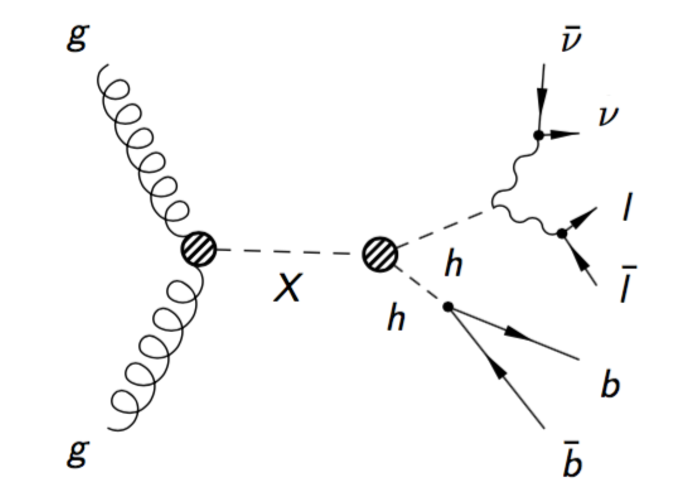
\includegraphics[width=0.45\textwidth]{BGtoHH.pdf}
    \caption{ The Feynman diagram of the graviton/radion production with the subsequent decay to HH. HH system decays to a pair of b quarks and Z bosons. Shown is 2 b quarks, 2 leptons, and 2 neutrinos final state.
    }
    \label{fig:BGtoHH}
  \end{center}
\end{figure}


\section{Analysis Strategy}

The analysis is based on ntuples and object selection from the approved VHbb sister analysis~\cite{VHbb_inspire}. Leptons, b jets, and the missing transverse energy (MET) are reconstructed using the standard CMS procedures~\cite{CMSreco} and the Particle Flow (PF) algorithm~\cite{PFalgo}. b-jets are identified using the Combined MVA v2 (CMVA) algorithm~\cite{BTagtwiki}. Then, on shell Z boson candidates are selected of dilepton pairs of the same flavour with a net charge zero for a pair. Higgs boson candidate decaying to b quarks (Hbb) is reconstructed as a pair of b jets with the highest CMVA output value. Finally, double Higgs boson pseudo-transverse mass, which is used in the shape analysis to extract limits, is constructed computing the transverse mass of the sum of the Lorentz vectors of the two leptons forming the on-shell Z, MET, and a pair of the b jets forming the \HBB. Additionally, a cut on the missing transverse energy is introduced to preserves the orthogonality with the existing HIG-18-013 ``2b 2l 2q'' analysis, which also works with the $bbZZ$ decays. In a similar fashion, the cut on the Z mass ($m_Z > 76$ GeV) is used to orthogonalise the analysis with respect to the HH phase space used in the legacy $bbWW$ analysis where the final signature is identical to ours. Lastly, the cut on the BDT is used to reduce the background contamination in the signal region.

Main backgrounds are \ttbar and Drell-Yan in association with jets. To determine their normalization, we construct two dedicated control region, which are correspondingly \ttbar and Drell-Yan dominated. Then, during the the simultaneous fit of signal region (SR), as well as control region \ttbar (CRTT), and control region Drell-Yan (CRDY), we obtain rates for these processes. Others, minor backgrounds, are single top production, diboson samples (WW, WZ, ZZ), and ZH production and are determined from the Monte Carlo (MC) simulation. 
%We assign systematics uncertainties on the QCD scale corresponding to each process. Also uncertainty associated with the imperfect knowledge of the single top cross section is added.

In the next chapters we will discuss all of the aspects of the analysis in details starting with the chapter on Data. 


\section{Data and Triggers}
\label{sec:data_and_triggers}

\subsection{Data}
This measurement uses the full dataset of 2016 collected with the CMS detector in pp collisions
at 13 TeV center-of-mass energy with the corresponding integrated luminocity of 35.9 ~\fbinv. 

As the measurement is based on dilepton signatures, the DoubleMuon and DoubleElectron primary
datasets are analyzed and only on-shell \Zll~decays are considered, where $\ell=\Pe, \Pgm$. CMS delivered data in several runs. The run periods and the corresponding integrated luminosities are listed in Table ~\ref{tab:datasets} for DoubleMuon channel, DoubleElectron channel numbers are similar.

\begin{table}[htbp]
\caption{List of used 2016 DoubleMuon data sets.
%\lumi16  across all modes.  
An uncertainty of $2.5\%$ is  assigned for the 2016 data set luminosity~\cite{lumiUnc}}
\label{tab:datasets}
\begin{center}
\scalebox{0.8}{
\begin{tabular}{|c|c|} \hline%\hline
Dataset       & $\int\mathcal L$ (\fbinv) \\
\hline
%{\texttt DoubleMuon\_Run2016B-03Feb2017-v1}       & \multirow{2}{*}{$\sim$5.9}  \\
{\texttt DoubleMuon\_Run2016B-03Feb2017-v2}       & {$\sim$5.9}  \\
%{\texttt DoubleMuon\_Run2016B-03Feb2017-v2}       &   \\
{\texttt DoubleMuon\_Run2016C-03Feb2017-v1}       & $\sim$2.7 \\
{\texttt DoubleMuon\_Run2016D-03Feb2017-v1}       & $\sim$4.3 \\
{\texttt DoubleMuon\_Run2016E-03Feb2017-v1}       & $\sim$4.1 \\
{\texttt DoubleMuon\_Run2016F-03Feb2017-v1}       & $\sim$3.2 \\
{\texttt DoubleMuon\_Run2016G-03Feb2017-v1}       & $\sim$3.8 \\
{\texttt DoubleMuon\_Run2016H-03Feb2017-v1}       & $\sim$11.8 \\
\hline
Total Lumi                        & 35.9 \\
\hline%\hline
\end{tabular}
}
\end{center}
\end{table}

\subsection{Triggers\label{sec:triggers}}
%% Because the analysis is performed in the dielectron and dimuon channels, unprescaled dilepton 
%% triggers with the lowest available transverse momentum thresholds are utilized. The triggers at the L1 and
%% HLT level are listed in table ~\\ref{tab:trgs2015}. Dielectron trigger requires the leading electron to pass $23$ GeV $p_{T}$ cut and $12$ GeV $p_{T}$ cut for the subleading electron. Offline cuts are $25$ GeV $p_{T}$ cut and $15$ GeV $p_{T}$ cut correspondinly. Dimuon triggers require the leading muon to pass $17$ GeV $p_{T}$ cut and $8$ GeV $p_{T}$ cut for the subleading muon with the $20$ GeV $p_{T}$ cut and $15$ GeV $p_{T}$ cut for offline selection correspondinly. $\eta$ region in the gap is excluded (1.4442 to 1.566). 

The rate at which particles are produced at LHC is not suitable for a direct persistence to the tape, it is too high and contains lots of uninteresting events. Therefore, we need a "trigger" that can select the potentially interesting events, such as those which will produce the Higgs particle or a Z/W boson, etc. In parallel, trigger also reduces the rate to just a few hundred "events" per second, which can be read out and stored on computer disk for subsequent offline analysis. Our $bbZZ$ analysis is performed in the dielectron and dimuon channels, so low momentum events are important to us. That is why unprescaled dilepton triggers with the lowest available transverse momentum thresholds are utilised. The triggers at the level 1 (L1) and high level trigger (HLT) are listed in Table ~\ref{tab:trgs2015}. Dielectron trigger requires the leading electron to pass $23$ GeV $p_{T}$ cut and the trailing (subleading) electron to pass $12$ GeV $p_{T}$ cut, both electrons should be within $\eta < $ 2.5. Dimuon triggers require the leading muon to pass $17$ GeV $p_{T}$ cut and $8$ GeV $p_{T}$ cut for the subleading muon, both muons should be within $\eta < $  2.4. The $\eta$ region (1.4442 to 1.566) in the gap between the barrel and endcap is excluded.



\begin{table}[b]
\caption{Triggers for dimuon and dielectron analysis channels both at L1 and HLT levels.}
% In parenthesis we report the threshold used for data after run2016D.                                                                                                                                    

\label{tab:trgs2015}
\begin{center}
\scalebox{0.75}{
\begin{tabular}{|c|c|c|} \hline%\hline
 Channel                    & L1 Seeds                 & HLT Paths                                                         \\ \hline
 Z$(\Pgm\Pgm)$~\Znn \HBB       & {\texttt L1\_SingleMu20}          & {\texttt HLT\_Mu17\_TrkIsoVVL\_Mu8\_TrkIsoVVL\_v* OR}                    \\
                              & { }                        & {\texttt HLT\_Mu17\_TrkIsoVVL\_TkMu8\_TrkIsoVVL\_v* OR}         \\
                              & { }                        & {\texttt HLT\_Mu17\_TrkIsoVVL\_Mu8\_TrkIsoVVL\_DZ\_v* OR}         \\
                              & { }                        & {\texttt HLT\_Mu17\_TrkIsoVVL\_TkMu8\_TrkIsoVVL\_DZ\_v*}         \\ \hline
 Z$(\Pe\Pe)$~\Znn \HBB         & {\texttt L1\_SingleEG30      OR}  & {\texttt HLT\_Ele23\_Ele12\_CaloIdL\_TrackIdL\_IsoVL\_DZ } \\
                              & {\texttt L1\_SingleIsoEG22er OR}  & {  }         \\
                              & {\texttt L1\_SingleIsoEG24   OR}  & {  }         \\
                              & {\texttt L1\_DoubleEG\_15\_10  }  & {  }         \\ \hline
%\hline%\hline
\end{tabular}
}
\end{center}
\end{table}

Due to the fact that there are discrepancies between trigger efficiencies in data and in simulation, we need trigger scale factors. Before measuring them, identification (ID) and isolation (ISO) cuts should be applied. Identification criteria helps selecting real prompt leptons, which isolation criteria stresses the fact that a track for the real prompt lepton should be isolated from the other activity nearby. Further, $p_{T}$ cuts of the offline selection are replicated. For dielectron trigger leading and subleading electrons have to pass $25$ GeV $p_{T}$ cut and $15$ GeV $p_{T}$ cut correspondinly. Dimuon triggers require the leading muon to pass $20$ GeV $p_{T}$ cut and $15$ GeV $p_{T}$ cut for the subleading muon. 
Dilepton scale factor have been computed for each leg separately, since the cuts on each leg vary (Fig. ~\ref{fig:trigger_eff_diele}). Following the recommendations from the Muon Particle Object Group (POG), scale factors have been computed separately for two groups: run H and other runs, and then the final scale factors are determined as luminosity averaged scale factors (Figs. ~\ref{fig:trigger_SF_dimu_BCDEFG}, ~\ref{fig:trigger_SF_dimu_H}, ~\ref{fig:trigger_SF_dimu_dZ_H}). Muon ID, ISO, and electron ID$+$ISO scale factors are shown at Figs. \ref{fig:muonID_SF}, \ref{fig:muonISO_SF}, \ref{fig:eleIDnISO_SF}.


\begin{figure}
\centering
\subfloat Leg 1
{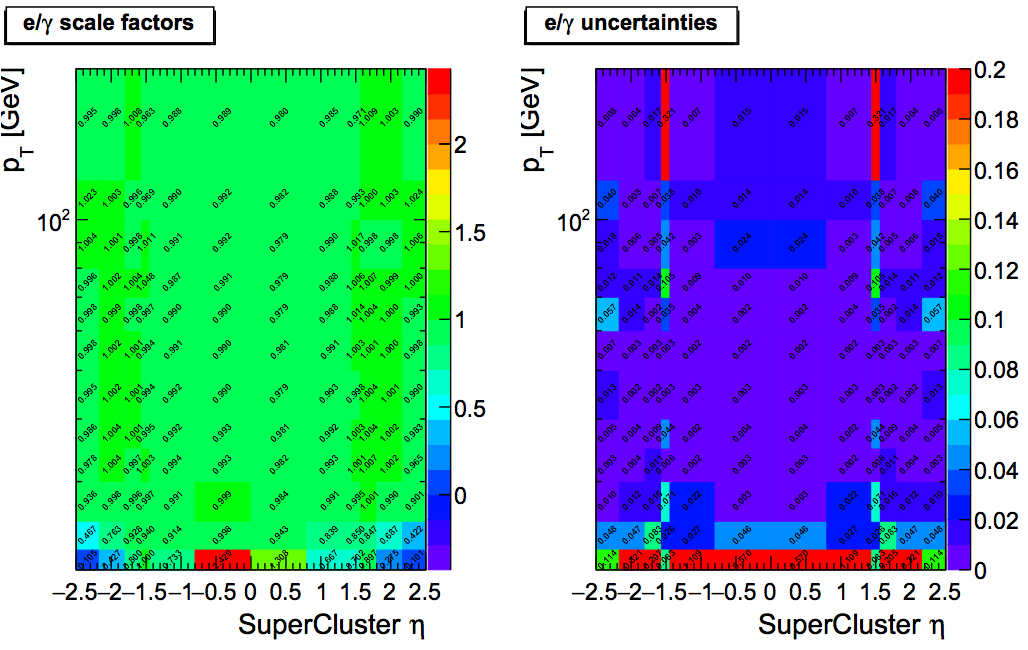
\includegraphics[width=1.0\textwidth]{trigger/electronTriggerEfficiencyelectronTriggerEfficiencyHLT_Leg1_WP90_2016.png} } \\
\subfloat Leg 2
{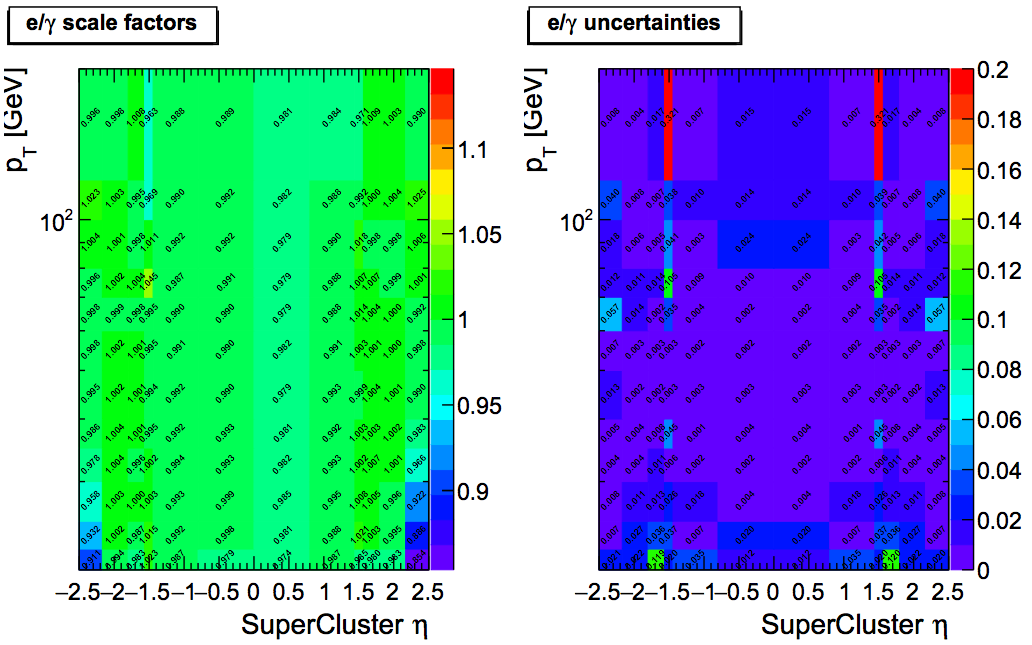
\includegraphics[width=1.0\textwidth]{trigger/electronTriggerEfficiencyelectronTriggerEfficiencyHLT_Leg2_WP90_2016.png} } \\
\caption{Electron scale factors in $p_{T}$ and $\eta$ bins for 2016 data set for the HLT\_Ele23\_Ele12\_CaloIdL\_TrackIdL\_IsoVL\_DZ trigger. ID cut (general purpose MVA WP90) and ISO cuts are applied, then the scale factors are measured. Taken from ~\cite{vhbbAN}}
\label{fig:trigger_eff_diele}
\end{figure}


\begin{figure}
\centering
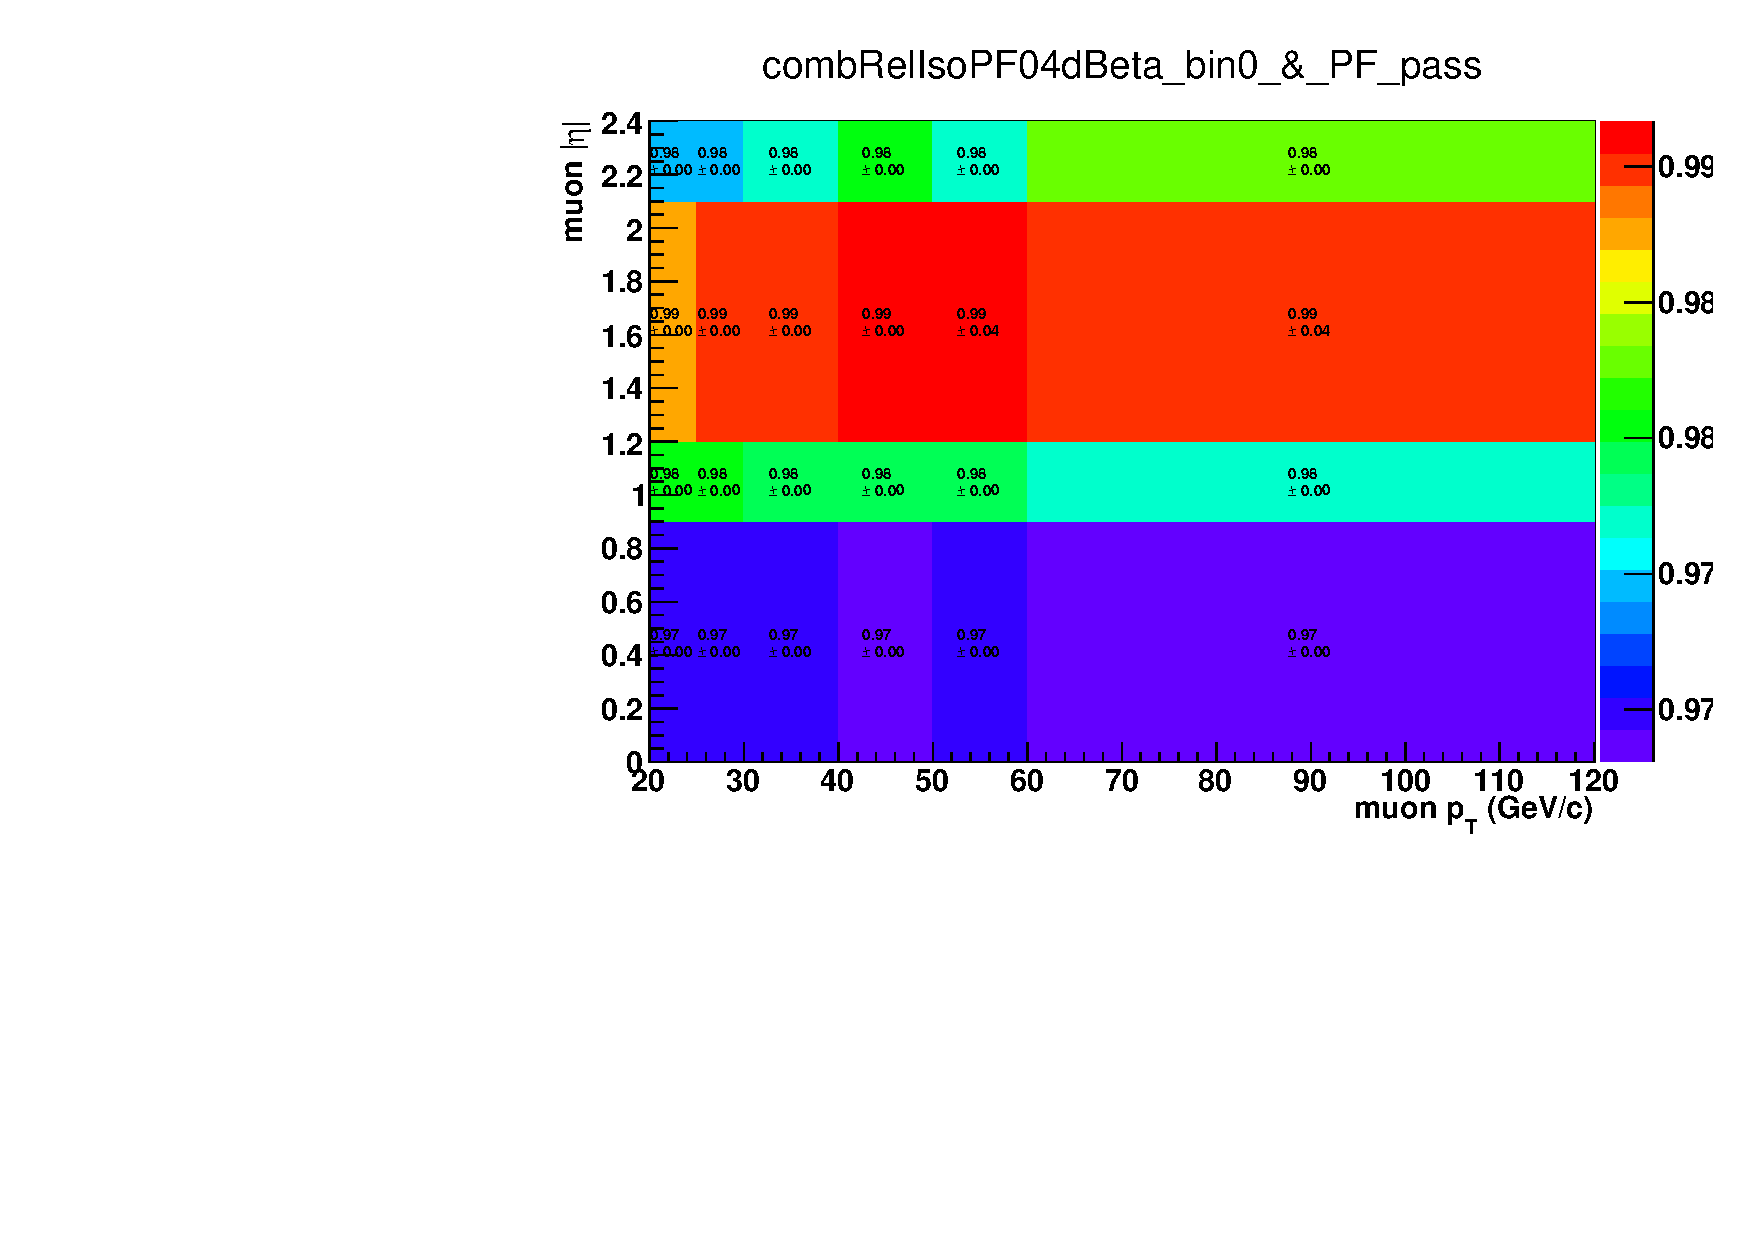
\includegraphics[width=0.475\textwidth]{trigger/Run_BCDEFG_PlotSF_hlt_Mu17_Mu8_OR_TkMu8_leg8_NUM_hlt_Mu17_Mu8_OR_TkMu8_leg8_DEN_LooseIDnISO_PAR_pt_eta_pt_abseta_ratio.pdf}
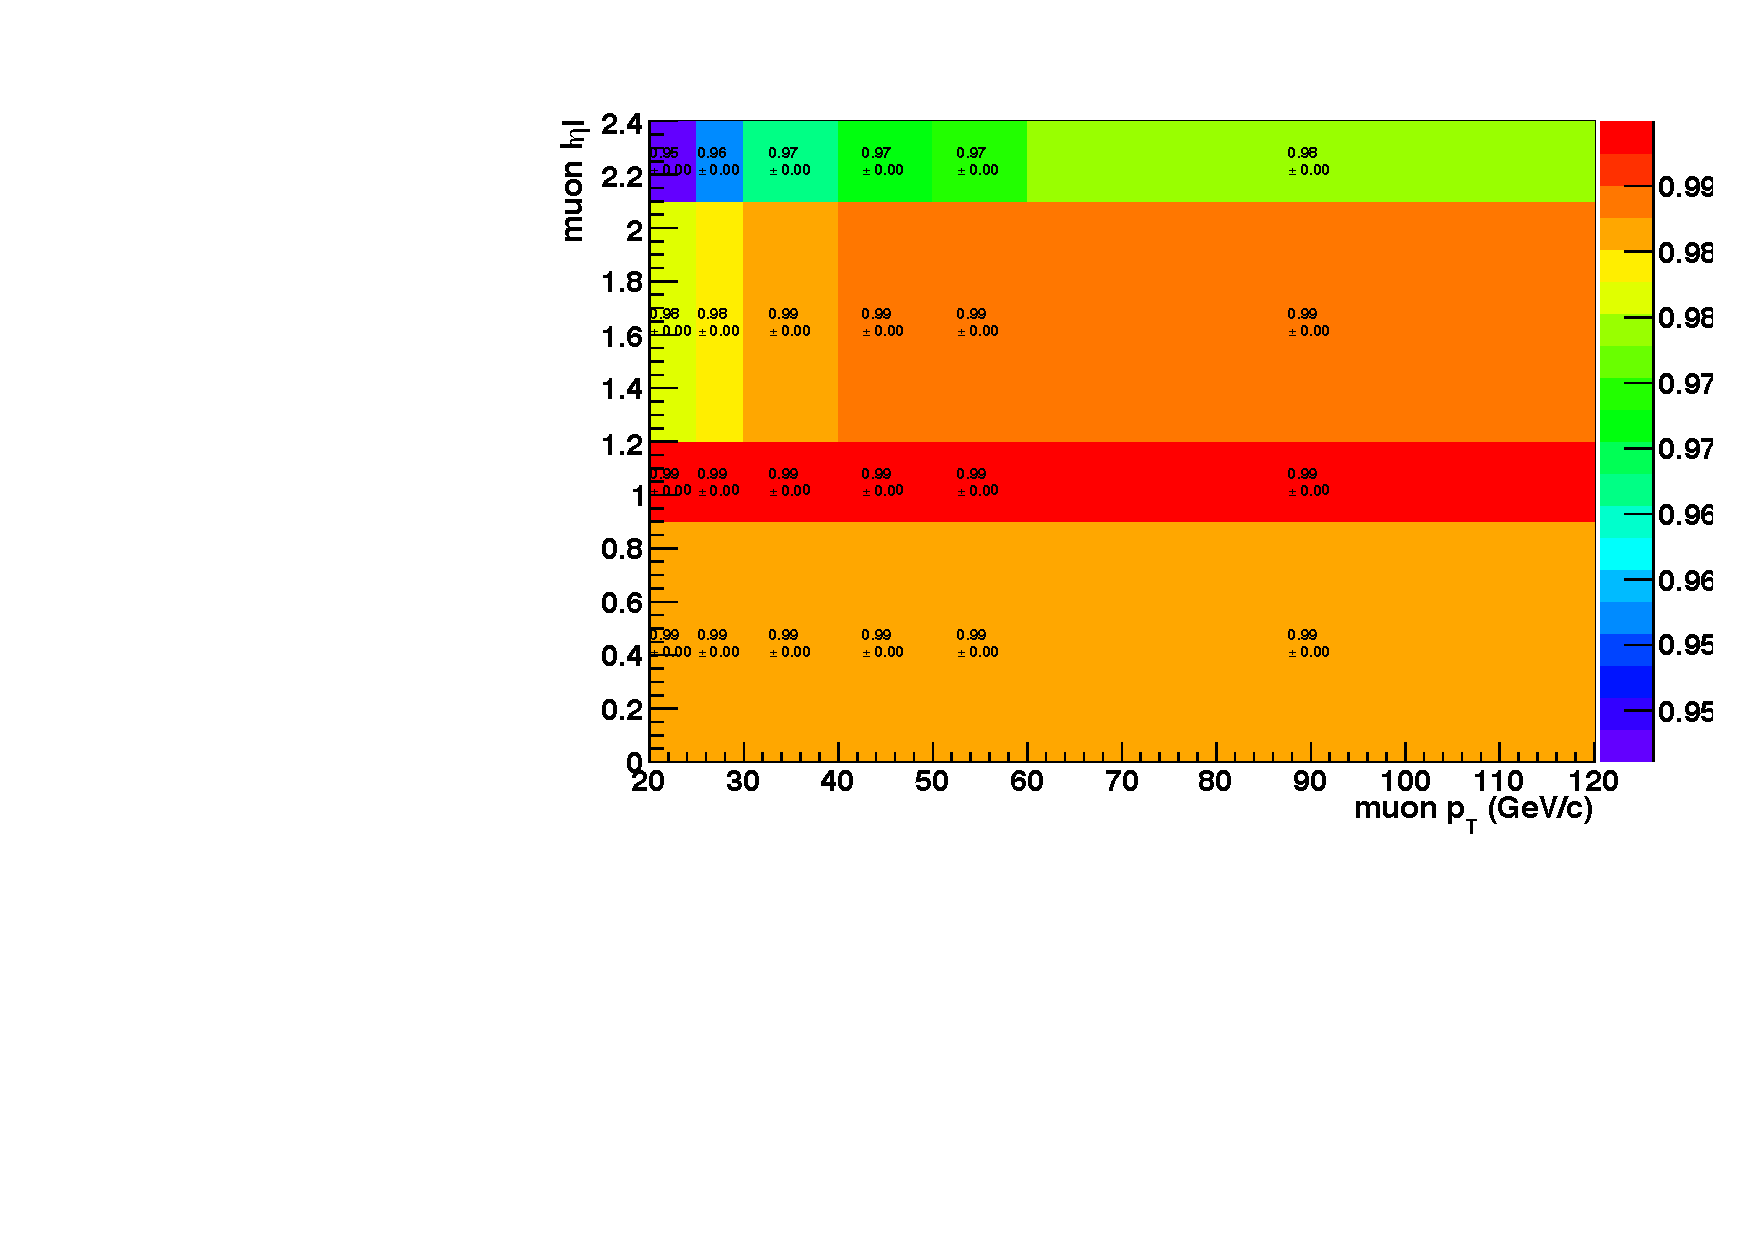
\includegraphics[width=0.475\textwidth]{trigger/Run_BCDEFG_PlotSF_hlt_Mu17Mu8_leg17_NUM_hlt_Mu17Mu8_leg17_DEN_LooseIDnISO_PAR_pt_eta_pt_abseta_ratio.pdf}\\
\caption{Muon scale factors in $p_{T}$ and $\eta$ bins for 2016 data runs B, C, D, E, F, G for the  HLT\_Mu17\_TrkIsoVVL\_Mu8\_TrkIsoVVL\_v* OR HLT\_Mu17\_TrkIsoVVL\_TkMu8\_TrkIs\
oVVL\_v* triggers. Left: Scale factors for 8 GeV leg. Right: Scale factors for 17 GeV leg, provided that the subleading leg passed 8 GeV cut.}
\label{fig:trigger_SF_dimu_BCDEFG}
\end{figure}

\begin{figure}
\centering
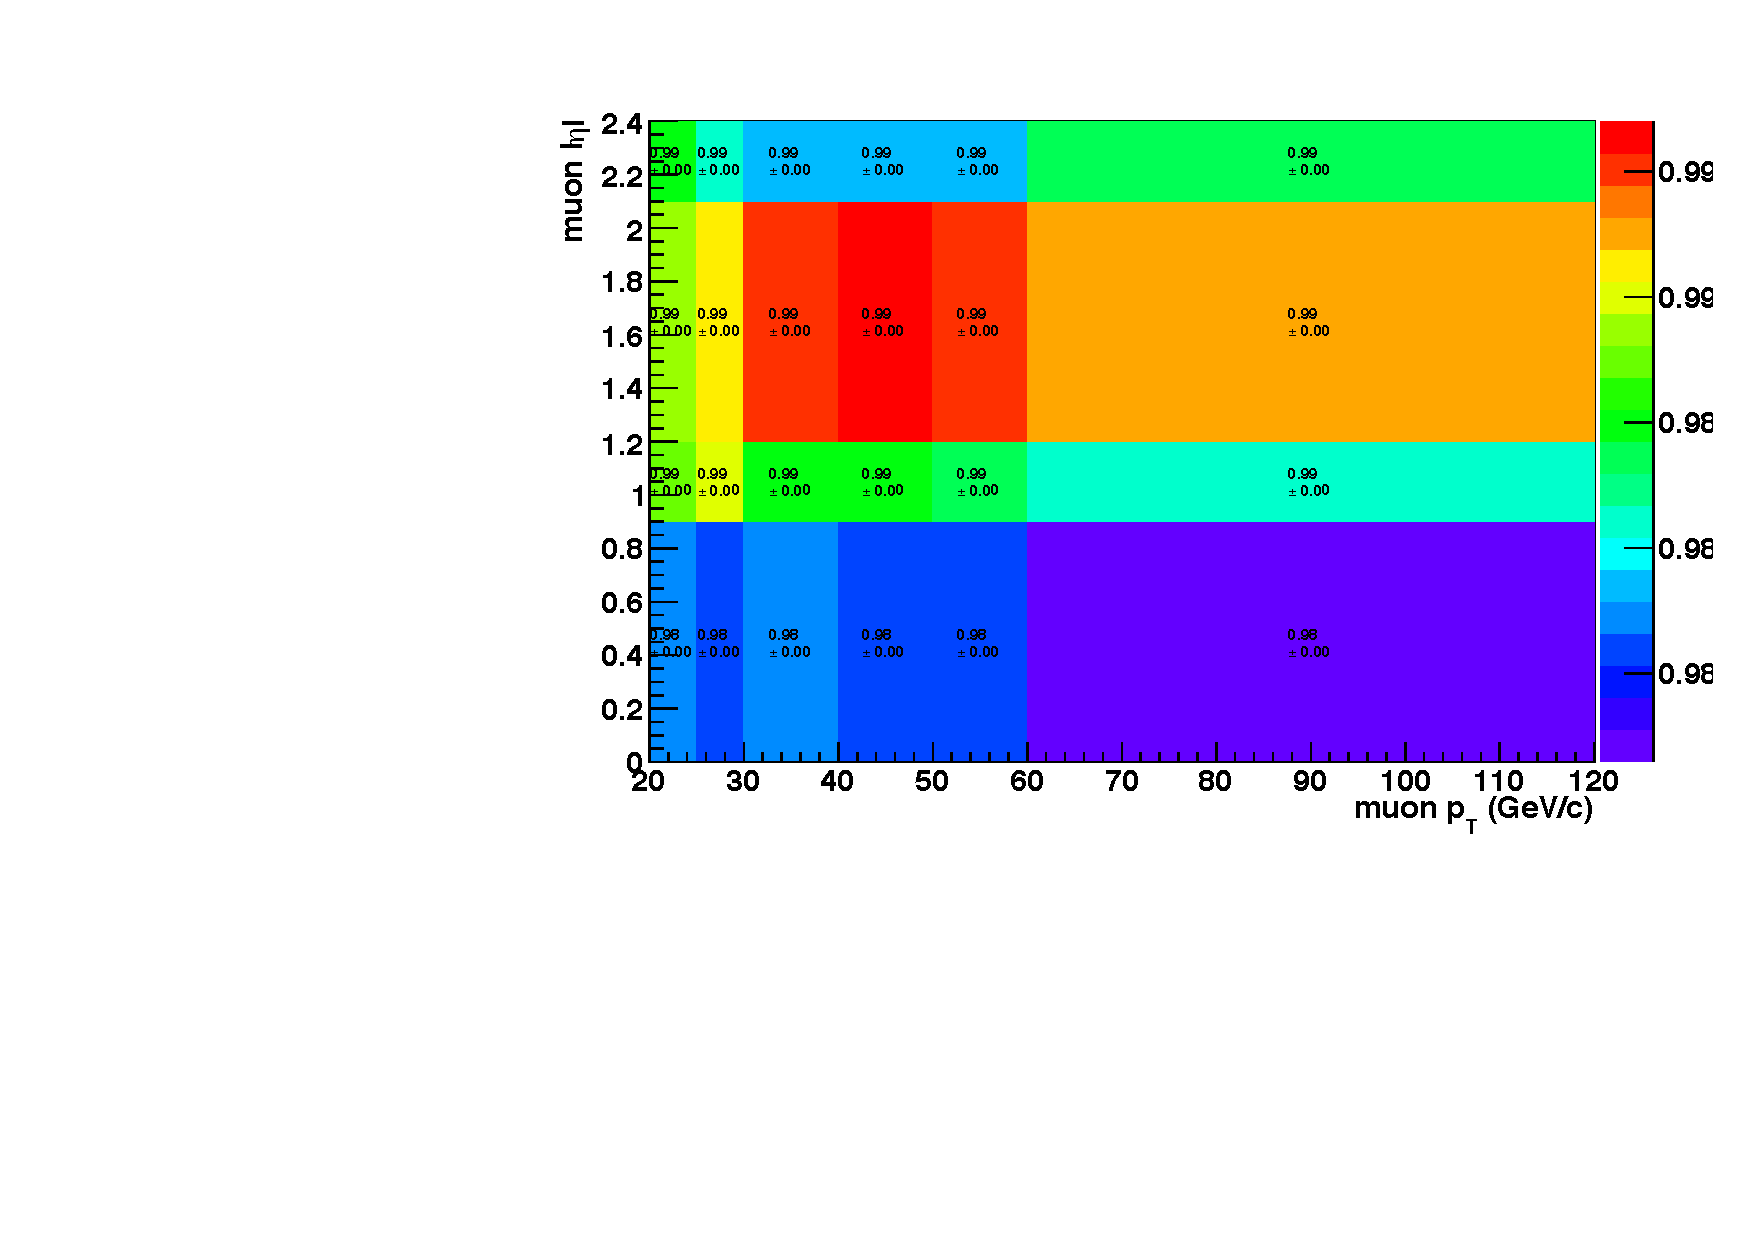
\includegraphics[width=0.475\textwidth]{trigger/Run_H_PlotSF_hlt_Mu17_Mu8_OR_TkMu8_leg8_NUM_hlt_Mu17_Mu8_OR_TkMu8_leg8_DEN_LooseIDnISO_PAR_pt_eta_pt_abseta_ratio.pdf}
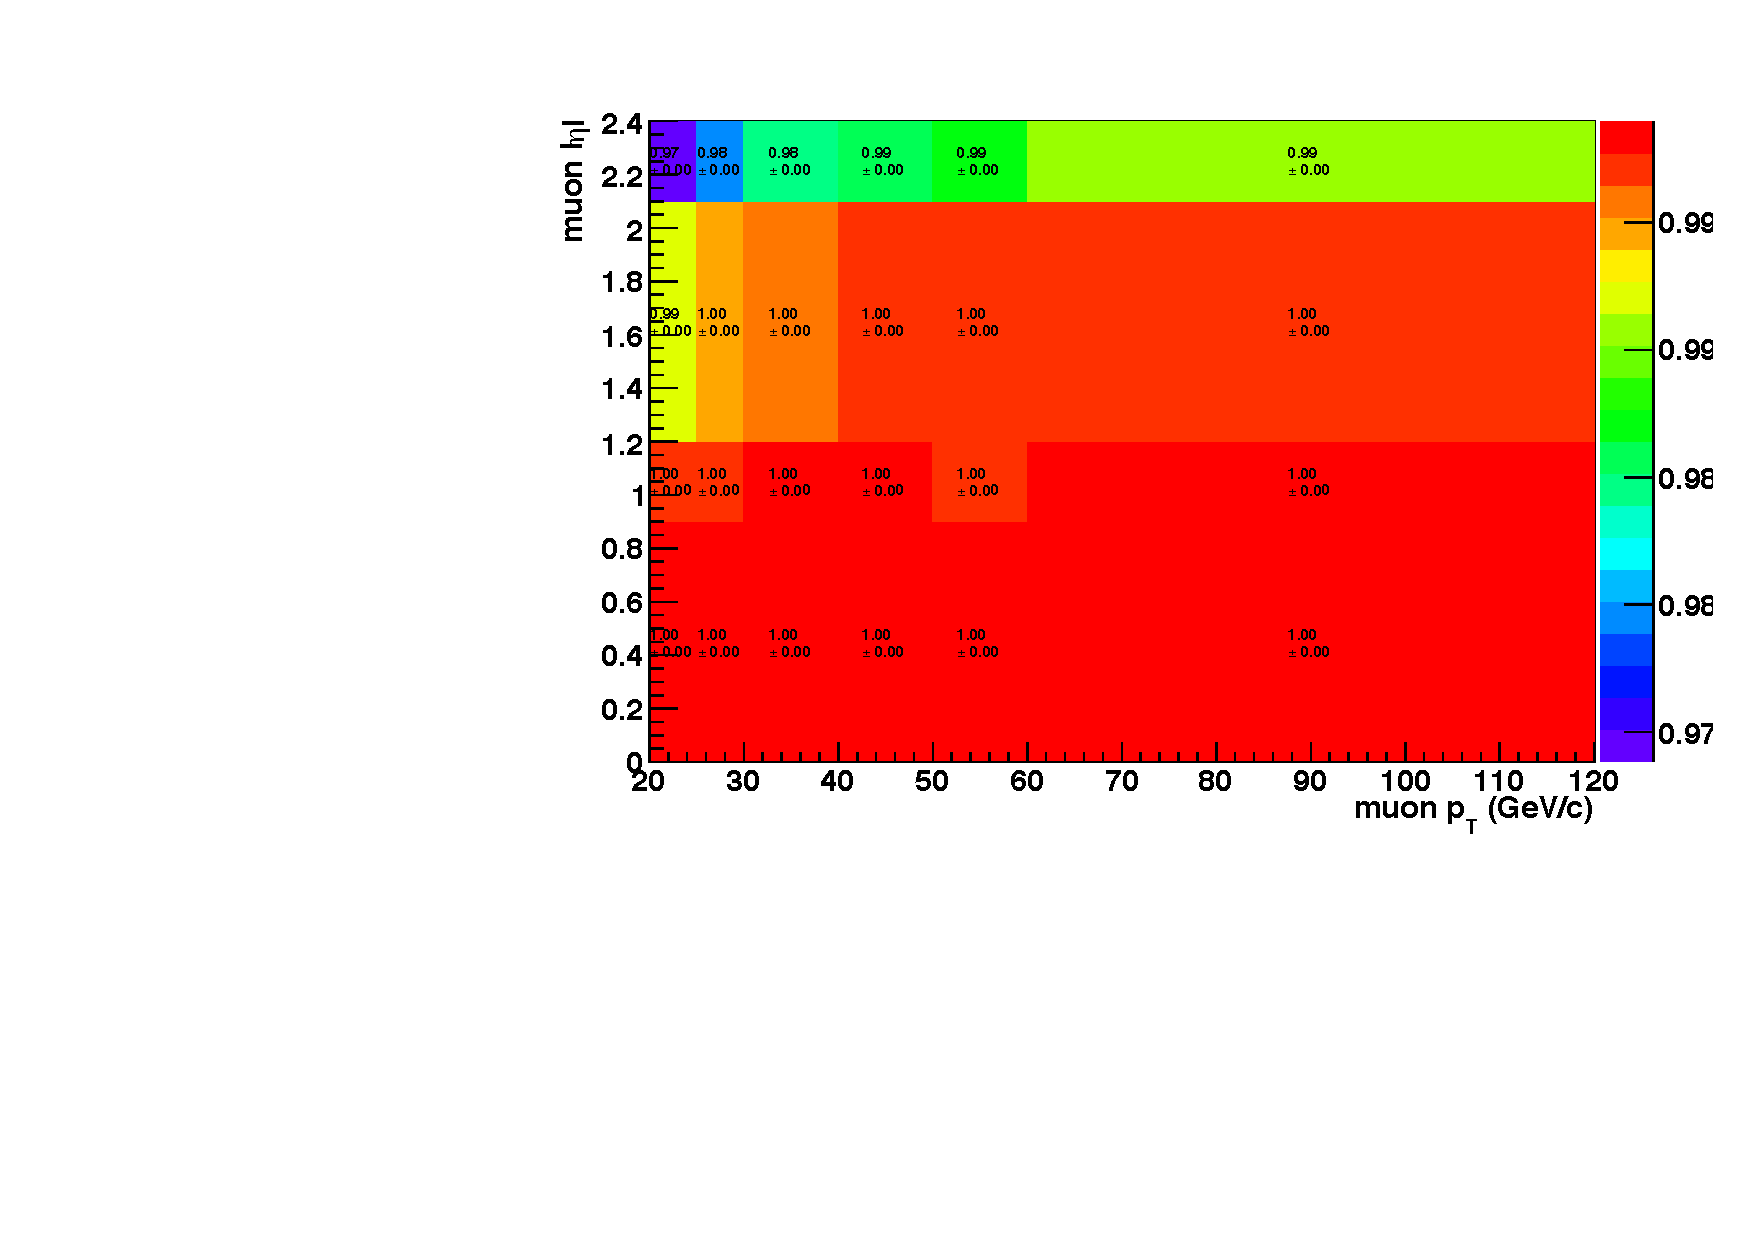
\includegraphics[width=0.475\textwidth]{trigger/Run_H_PlotSF_hlt_Mu17Mu8_leg17_NUM_hlt_Mu17Mu8_leg17_DEN_LooseIDnISO_PAR_pt_eta_pt_abseta_ratio.pdf}\\
\caption{Muon scale factors in $p_{T}$ and $\eta$ bins for 2016 data run H for the  HLT\_Mu17\_TrkIsoVVL\_Mu8\_TrkIsoVVL\_v* OR HLT\_Mu17\_TrkIsoVVL\_TkMu8\_TrkIs\
oVVL\_v* triggers. Left: Scale factors for 8 GeV leg. Right: Scale factors for 17 GeV leg, provided that the subleading leg passed 8 GeV cut.}

\label{fig:trigger_SF_dimu_H}
\end{figure}

\begin{figure}
\centering
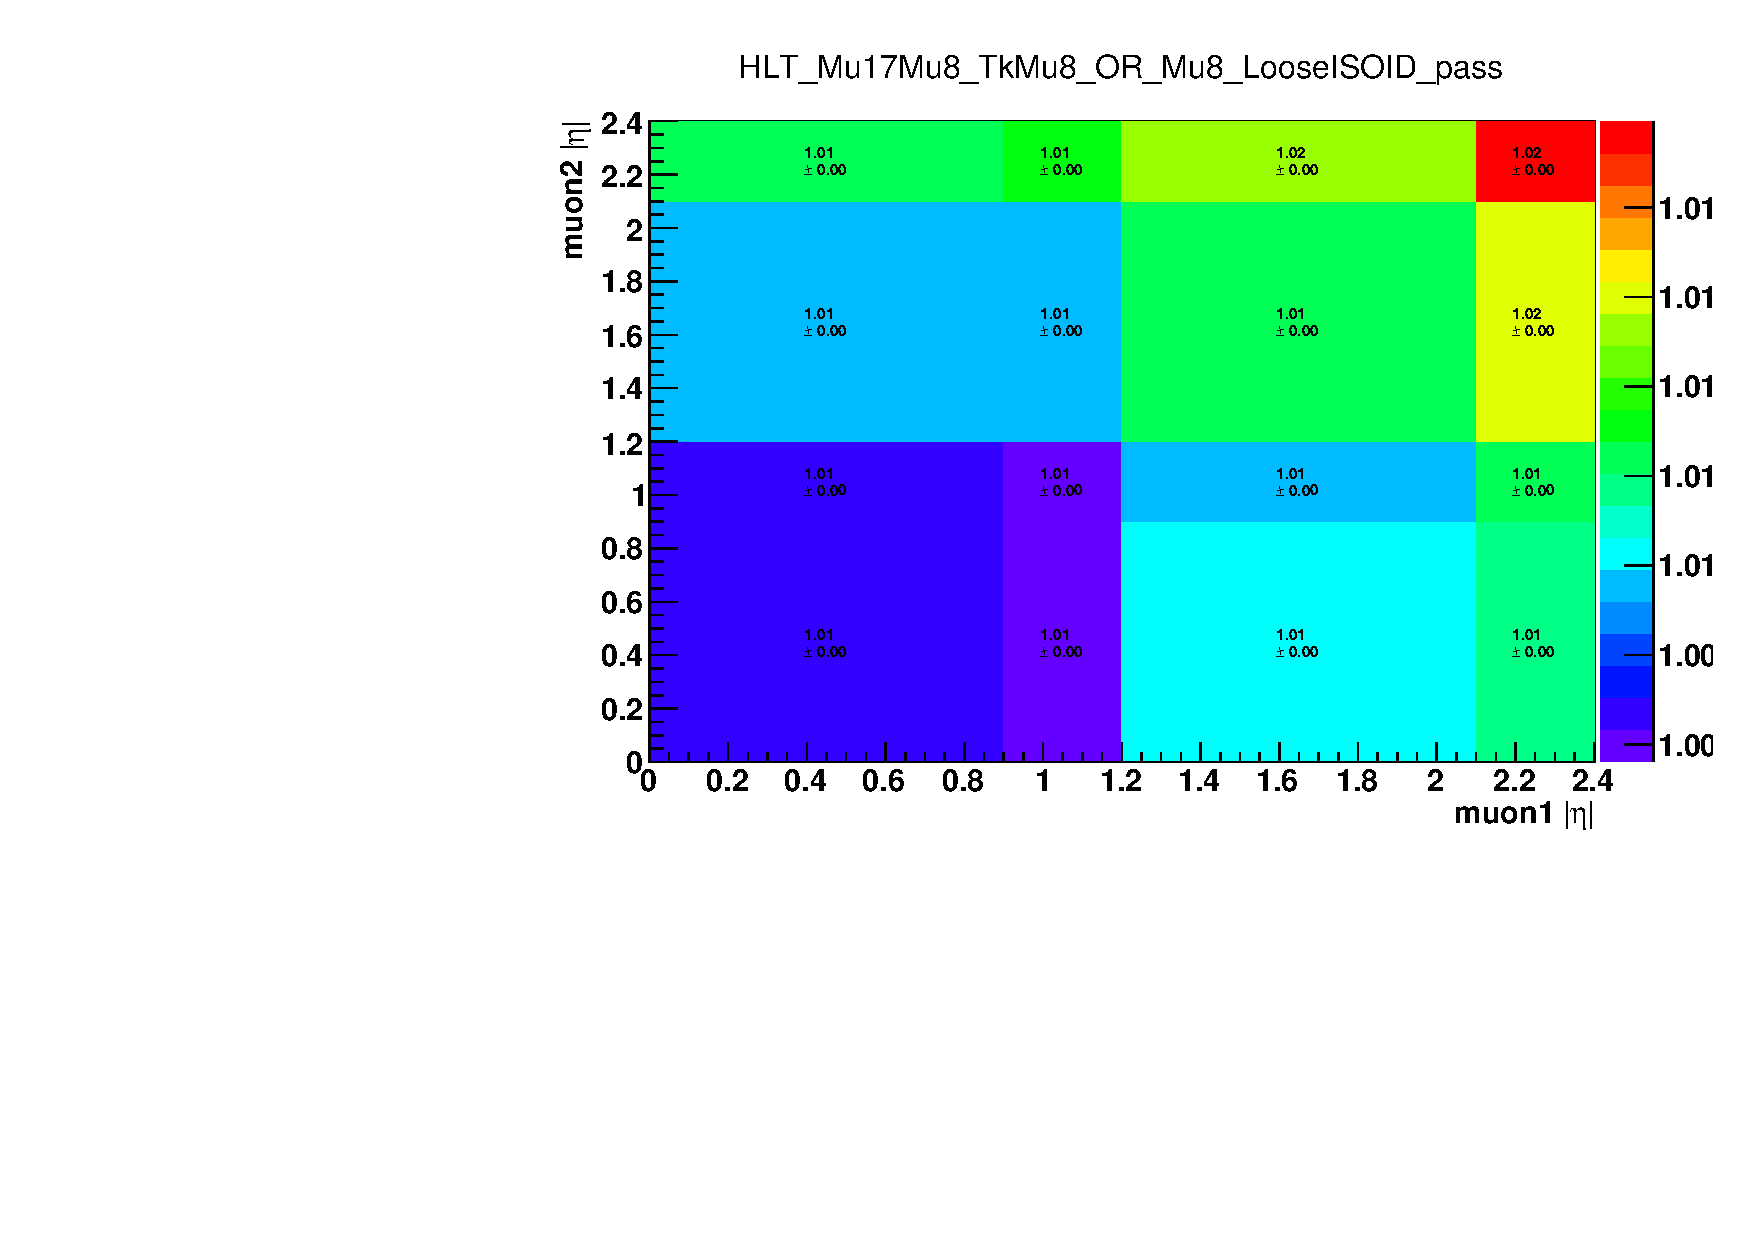
\includegraphics[width=0.85\textwidth]{trigger/PlotSF_dZ_NUM_dZ_DEN_hlt_Mu17_Mu8_OR_TkMu8_loose_PAR_eta1_eta2_abseta_tag_abseta_ratio.pdf}
\caption{Scale factors in $\eta$ bins of the leading and subleading muons for 2016 data set for dZ requirement, measured after muons have passed the HLT\_Mu17\_TrkIsoVVL\_Mu8\_TrkIsoVVL\_v* OR HLT\_Mu17\_TrkIsoVVL\_TkMu8\_TrkIsoVVL\_v* triggers. }
\label{fig:trigger_SF_dimu_dZ_H}
\end{figure}




\begin{figure}
\centering
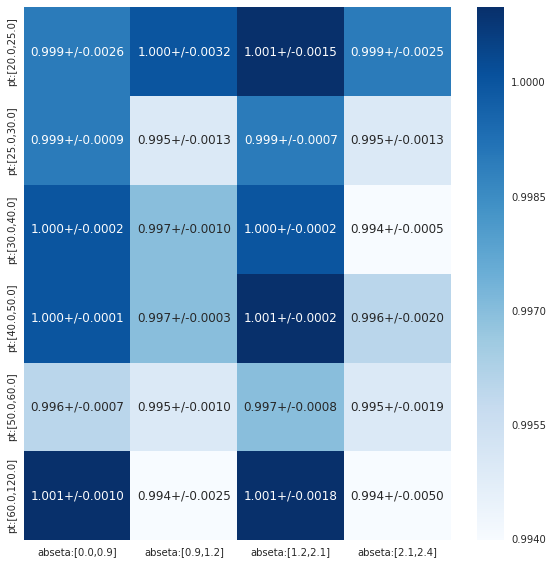
\includegraphics[width=0.5\textwidth]{muon_ID_BCDEFv2.png}
\bigbreak
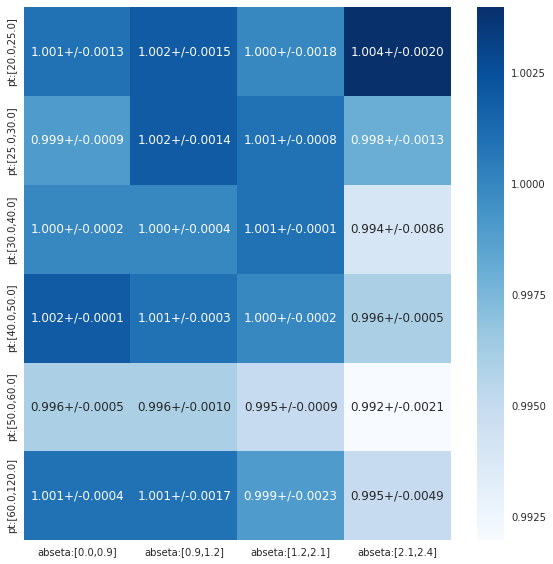
\includegraphics[width=0.5\textwidth]{muon_ID_GHv2.png}
\caption{ Muon ID scale factors in $p_{T}$ and $\eta$ bins. Left: runs B to F. Right: runs G and H.}
\label{fig:muonID_SF}
\end{figure}


\begin{figure}
\centering
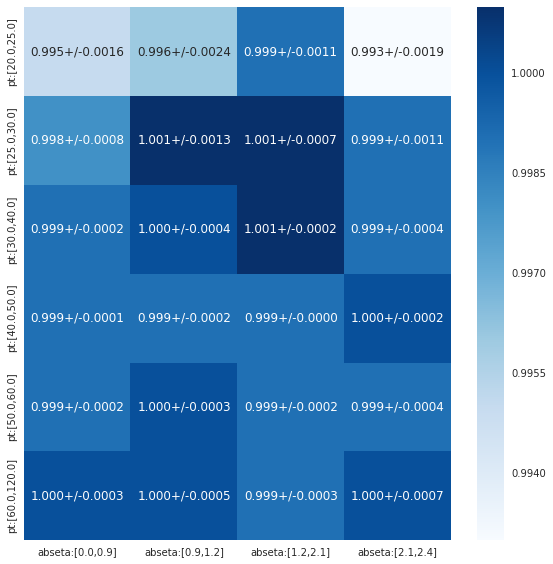
\includegraphics[width=0.5\textwidth]{muon_ISO_BCDEFv2.png}
\bigbreak
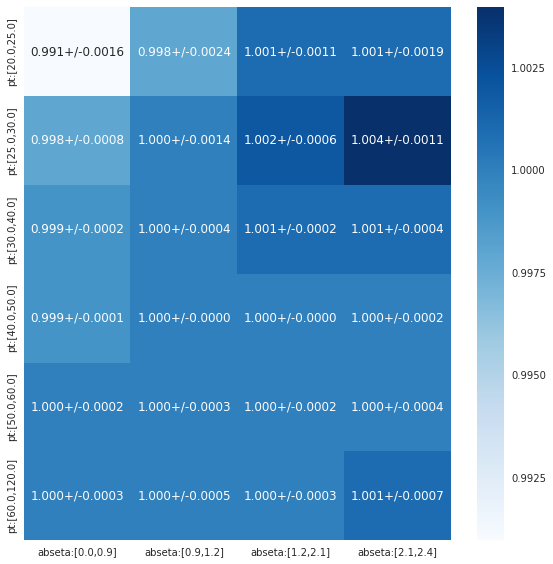
\includegraphics[width=0.5\textwidth]{muon_ISO_GHv2.png}
\caption{ Muon ISO scale factors in $p_{T}$ and $\eta$ bins. Left: runs B to F. Right: runs G and H.}
\label{fig:muonISO_SF}
\end{figure}

\begin{figure}
\centering
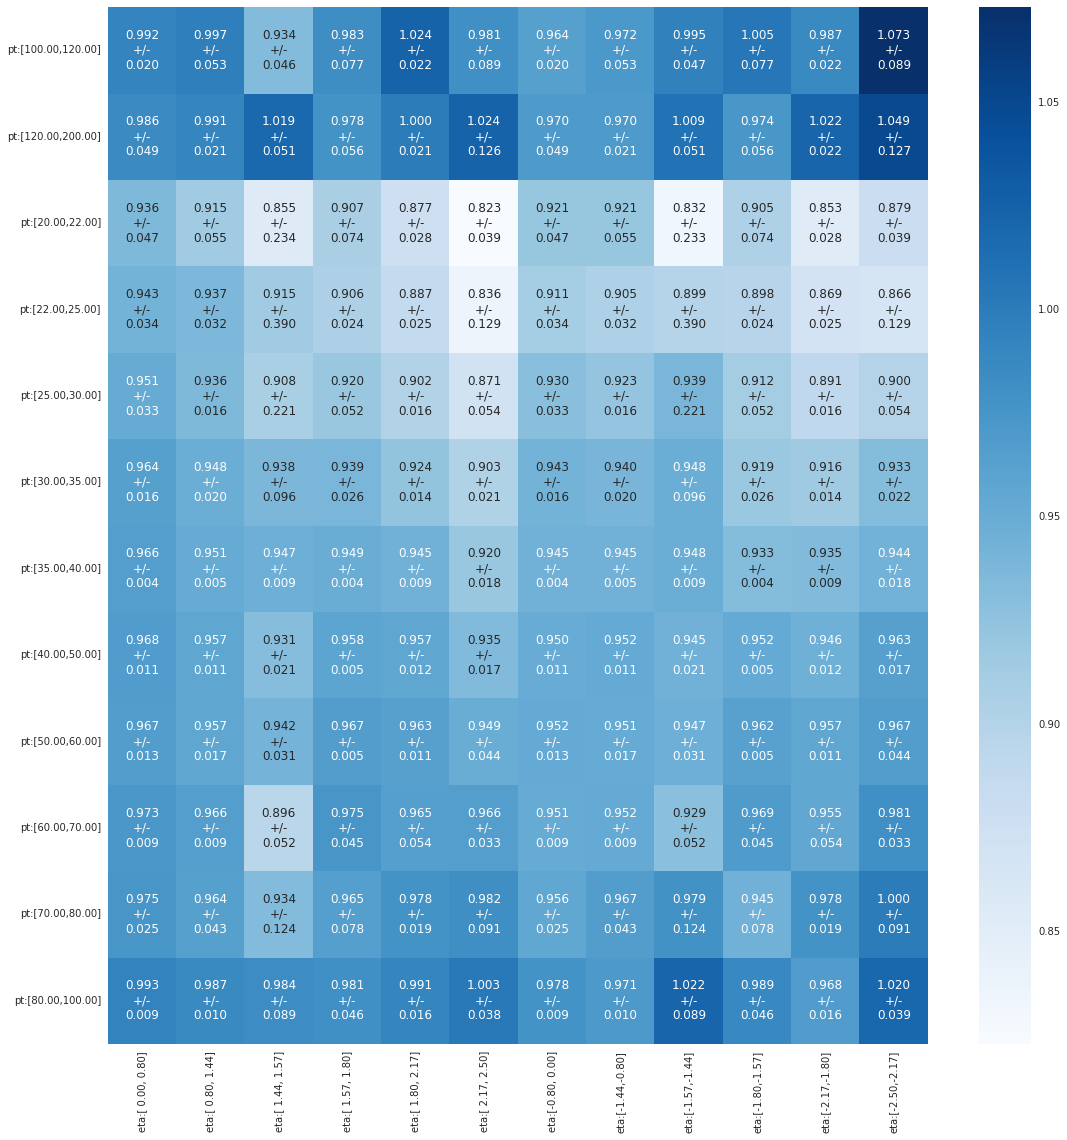
\includegraphics[width=0.9\textwidth]{EIDISO_ZH_out.png}
\caption{ Electron ID+ISO scale factors in $p_{T}$ and $\eta$ bins.}
\label{fig:eleIDnISO_SF}
\end{figure}



\section{Simulated Samples}
\label{sec:simulated_samples}
%\section{Monte~Carlo samples\label{sec:mc}}

Before we look at the data, all the studies are done with the simulation. The most important requirements on the simulation is that it is accurate and has enough events in all the phase space corners. While this is almost true for the main backgrounds, for which the simulated samples are produced centrally for the use of the whole CMS, specific signal samples cannot be produced with big statistics for all analyses, since there are hundred analysis teams in CMC. Luckily for us, both $bbZZ$ and $bbWW$ samples have been produced with $O$(0.5 M events).

\subsection{Signal simulation\label{sec:signalMC}}




MC signal samples of the resonant Higgs boson pair production have been generated at the Leading Order (LO) using the \MADGRAPH~5 version\ ~2.2.2.0  generator ~\cite{Alwall:2014hca}. The gluon fusion production of a heavy narrow resonance is followed by the decay of the resonance into two SM Higgs bosons whose mass is fixed at 125~GeV.

Two signal MC samples are generated to cover the Higgs decay modes contributing to the 2 b jets 2 leptons 2 neutrinos final state of this measurement. The first sample type is a HH decay in to bbZZ channel, where one Higgs boson decays to a pair of b-quarks and the second Higgs boson decays into two Z bosons. In the second sample type bbVV events are generated, where HH can decay through bbWW and bbZZ channels. For both samples, the Z boson-pair and the W boson-pair are set to decay leptonically to two leptons and two neutrinos, where a lepton could be an electron or a muon. The second, bbVV, sample is filtered using the generator level information such that only the events with a W-boson pair (bbWW) are kept, while the Z-pair events are dropped: there are very few of them in the bbVV sample, and most importantly, high statistics bbZZ is taken from the dedicated bbZZ sample of the first type.

Events in the signal bbZZ and bbWW MC samples are normalised to 2~pb HH production cross section, which is a typical value of the heavy resonance production at 300 GeV predicted by the WED. Additionally the normalization includes the branching ratios of the Higgs boson decays contributing to the final state studied here: 0.0012 and 0.0266 for $HH\to bbZZ\to bb\ell\ell\nu\nu$ and $HH\to bbWW\to bb\ell\nu\ell\nu$, respectively \cite{CERNYR4}.

%%There are ten samples in the mass range of 260 to 1000 GeV generated for bbVV analysis and 16 samples for bbZZ from 250 GeV to 1000 GeV. Therefore, this document presents results for the masses where both signals are present. In the future we would consider doing approximations of the bbWW contribution where we have missing samples or generate them privately.

Unless mentioned otherwise, throughout the text plots and numbers represent the graviton study. The data and backgrounds for the radion measurement are the same, thus distributions also show the same good Data MC agreement and can be found for at Figs. ~\ref{fig:MCcomparisons} for the graviton case and ~\ref{fig:MCcomparisons_radion} for the radion case.

\subsection{Background simulation\label{sec:bkgMC}}

In this analysis the main backgrounds are \ttbar and Drell-Yan plus
jets with the mass of the boson greater than 50 GeV. Not all the
background processes pass our tight preselection (see section ~\ref{sec:selection}),
those which do, are single top, dibosons, and ZH backgrounds that are
listed in the Table \ref{tab:bg_mcsamples}:

\begin{table}[htbp]%H]
  %\footnotesize
  %\begin{center}
    \caption{Background Monte Carlo samples\label{tab:bg_mcsamples}}
     %\scalebox{0.8}{
    \begin{tabular}{lc}%|l|r|r|r|r|r|}
      \hline
      % Sample  & Generator & $m_{H} (\GeV/c^2)$ & $\sigma$ (pb) & events &  $\int\cal L$ (\fbinv) \\
      %\hline
      %\multicolumn{5}{|l|}
      {\texttt{DY1JetsToLL\_M-50\_TuneCUETP8M1\_13TeV-madgraphMLM-pythia8}} \\
%                & \MADGRAPH\,5+\PYTHIA{}\,8 & 725 & 39 800 000 & 54.5 \\
      %\multicolumn{5}{|l|}
      {\texttt{DY2JetsToLL\_M-50\_TuneCUETP8M1\_13TeV-madgraphMLM-pythia8}} \\
%               & \MADGRAPH\,5+\PYTHIA{}\,8 & 725 & 39 800 000 & 54.5 \\
      %\hline
      %\multicolumn{5}{|l|}
      {\texttt{DY3JetsToLL\_M-50\_TuneCUETP8M1\_13TeV-madgraphMLM-pythia8}} \\
%              & \MADGRAPH\,5+\PYTHIA{}\,8 & 394.5 & 19 400 000  & 50.2 \\
      %\hline
      %\multicolumn{5}{|l|}
      {\texttt{DY4JetsToLL\_M-50\_TuneCUETP8M1\_13TeV-madgraphMLM-pythia8}} \\
%             & \MADGRAPH\,5+\PYTHIA{}\,8 & 96.47 & 4 960 000 & 52.2 \\
      %\multicolumn{5}{|l|}
      {\texttt{WW\_TuneCUETP8M1\_13TeV-pythia8}} \\
%            & \PYTHIA{}\,8 & 118.7 & 993 640 &  8.37  \\
      %\hline
      %\multicolumn{5}{|l|}
      {\texttt{WZ\_TuneCUETP8M1\_13TeV-pythia8}} \\
%           & \PYTHIA{}\,8 & 47.13    &   1 000 000   &   21.22  \\
      %\hline
      %\multicolumn{5}{|l|}
      {\texttt{ZZ\_TuneCUETP8M1\_13TeV-pythia8}} \\
%          & \PYTHIA{}\,8 & 16.523     &   985 600   &   59.65  \\
       %\multicolumn{5}{|l|}
       {\texttt{ZH\_HToBB\_ZToLL\_M125\_13TeV\_aMC@NLO}} \\
      %\hline
      %\multicolumn{5}{|l|}
      {\texttt{TT\_TuneCUETP8M1\_13TeV-powheg-pythia8}} \\
       %         & \POWHEG+\PYTHIA{}\,8 & 831.76   & 187 626 200 + 97 994 442&  343  \\
      %\hline
      %\multicolumn{5}{|l|}
      {\texttt{ST\_tW\_top\_5f\_inclusiveDecays\_13TeV-powheg-pythia8\_TuneCUETP8M1}} \\
        %        & \POWHEG+\PYTHIA{}\,8 & 35.6   &   1 000 000   &   28.09  \\
      %\hline
      %\multicolumn{5}{|l|}
      {\texttt{ST\_tW\_antitop\_5f\_inclusiveDecays\_13TeV-powheg-pythia8\_TuneCUETP8M1}} \\
         %       & \POWHEG+\PYTHIA{}\,8 & 35.6   &   999 400   &   28.07  \\
      %\hline\hline
      %\multicolumn{5}{|l|}
      {\texttt{ST\_t-channel\_top\_4f\_leptonDecays\_13TeV-powheg-pythia8}} \\
          %      & \POWHEG+\PYTHIA{}\,8 & 136*0.325   &   999 400   &   22.6 \\
      %\hline
      %\multicolumn{5}{|l|}
      {\texttt{ST\_t-channel\_antitop\_4f\_leptonDecays\_13TeV-powheg-pythia8}} \\
           %     & \POWHEG+\PYTHIA{}\,8 & 81*0.325   & 1 695 400 &  64.4 \\
      %\hline\hline
      %\multicolumn{5}{|l|}
      {\texttt{ST\_s-channel\_4f\_leptonDecays\_13TeV-amcatnlo-pythia8}} \\
      %    & \POWHEG+\PYTHIA{}\,8 & 10.32   &   998 400   &   96.74  \\
\hline%\hline
    \end{tabular}
  %\end{center}
  %}
  %\label{backgrounds} 
\end{table}



The simulated samples of the background processes such as 
~\ttbar~\cite{Frixione:2007nw} and the single top tW and t-channel
production processes~\cite{Frederix:2012dh} are generated at the
next-to-leading order (NLO) with POWHEG~\cite{Alioli:2009je}, while
single top s-channel production process is generated at NLO with
\MADGRAPH. \ttbar and single top production cross sections are
rescaled to the next-to-next-to-leading order (NNLO). 
Drell-Yan (DY)
process samples in association with 1, 2, 3 or 4 jets are generated
at the leading order using \MADGRAPH with the MLM
matching~\cite{Alwall:2007fs} and rescaled to NNLO using~\textsc{fewz}
program~\cite{Gavin:2010az,Li:2012wna,Gavin:2012sy}. 

As for the electroweak (EWK) order, DY samples have been rescaled to EWK NLO order with the NLO/LO k-factor of 1.23~\cite{DYkfactor}. Diboson samples
are generated at LO with {\PYTHIA}8.212~\cite{Sjostrand:2007gs}.

The main background
       process, which involves SM Higgs boson, is an associated
       production of the Higgs boson with a Z boson (ZH).  ZH process
       is simultated using the generator
%{{\sc MadGraph5_aMC@NLO}}                                                                                                                                                                               
$MadGraph5\_aMC@NLO$
~\cite{cite_aMC@NLO} with FxFx
merging~\cite{Frederix:2012ps} and
rescaled to NNLO with
{\MCFM} generator~\cite{Campbell:2010ff}.


For LO and NLO samples NNPDF3.0 parton distribution functions (PDF)
set is used. {\POWHEG} and {\MADGRAPH} interfaced with
{\PYTHIA}8.212~\cite{Sjostrand:2007gs} are used for the parton
showering and hadronization steps. To describe the underlying event
CUETP9M1 set derived in \cite{Khachatryan:2015pea} is
used. \GEANTfour~\cite{GEANT4} is used to model the response of the
CMS detector.

All the final cross sections denoted as NNLO are calculated at NNLO QCD accuracies and have been computed with the tool they were generated with. They found to be in agreement with the values from the LHC Higgs cross section working group ~\cite{LHCHXSWG, xsecZH, xsecTT, xsecST, xsecVV}.

During the data taking in 2016 the average number of proton-proton interactions per bunch crossing was 24 (denoted as pile up later), and in MC samples this information has been introduced overlapping these interactions with the events of interest.



\section{Physics Objects Reconstruction}
\label{sec:objects}

\hyphenation{fa-shion}
\hyphenation{ener-gy}

This the first ever bbZZ analysis performed at CERN with the real data. We use the standard set of the CMS
reconstructed physics objects. Below, we describe reconstruction of
each separately: electrons, muons, jets and b jets, and MET.



\subsection{Electrons\label{sec:electrons}}
The Gaussian Sum Filter (GSF) algorithm is used to reconstruct
electrons ~\cite{Khachatryan:2015hwa}. GSF helps to estimate track parameters. The procedure starts as follows: a mixture of Gaussian distributions (normally about 4-6 components) \cite{GSF} is used to estimate the energy loss in each layer of the tracker. The energy loss is modelled by the Bethe-Heitler formula. Two most important track properties are then computed: a weighted mean and the most frequent value (mode). The first estimate is unbiased while the latter one has a smaller width. In practice, mostly one works with the mode. Gaussian mixtures are determined minimising either the absolute difference between the cumulative density functions (CDFs) of the model and of the Gaussian mixture, or the Kullback-Leibner distance, which is a logarithm of the ratio of the probability density functions (pdfs) of the model with respect to the mixture. Finally, the tracks are extrapolated further to the ECAL The measurement selects electrons, which pass the following selection: leading electron $\pt>25\GeV$ and subleading electron 
$\pt>15\GeV$, $|\eta|<2.5$, 
%$d_{xy}<0.05\cm$, $d_z<0.2\cm$ and 
an isolation cut of 0.06, for which the cone
of $0.3$ is used to compute the $\rho$-subtracted PF
isolation. Lepton isolation is calculated as a scalar sum of
the transverse momentum $(p_{T})$ of all the charged and
neutral hadrons as well as photons around the lepton
(excluding the cone) normalised to the $p_{T}$ of the lepton
itself. 
%POG recommended MVA ID WP Loose is further applied to the set of selected electrons.
%The cut on isolation in the measurement for electrons is $0.06$.

        
        %%To emulate the conditions of the HLT trigger, a set of offline cuts is applied further.

%% \texttt{pt>15 \& (}\\
%% \texttt{(abs(superCluster().eta)<1.4442 \& full5x5\_sigmaIetaIeta<0.012 \& }\\
%% \texttt{hcalOverEcal<0.09 \&}\\
%% \texttt{(ecalPFClusterIso/pt)<0.4 \& (hcalPFClusterIso/pt)<0.25 \&}\\
%% \texttt{(dr03TkSumPt/pt)<0.18 \& abs(deltaEtaSuperClusterTrackAtVtx)<0.0095 \&}\\
%% \texttt{abs(deltaPhiSuperClusterTrackAtVtx)<0.065) || }\\
%% \texttt{(abs(superCluster().eta)>1.5660 \& full5x5\_sigmaIetaIeta<0.033 \&}\\
%% \texttt{hcalOverEcal<0.09 \&}\\
%% \texttt{(ecalPFClusterIso/pt)<0.45 \& (hcalPFClusterIso/pt)<0.28 \&}\\
%% \texttt{(dr03TkSumPt/pt)<0.18)}\\
%% \texttt{).}

        On top of the selection defined above, a specific CMS Particle Object Group (POG) recommended working point (WP) is applied, which is a discriminant based on the a multivariate analysis (MVA) for classification of signal/background electrons. The WP consists of nearly 20 variables utilising the information from the impact point, tracks, and the ECAL: $\chi^2$ variables of the track and the quality of its estimate, $\delta \eta$, $\delta \phi$, energy of the 3 by 3 cluster, ECAL energy over momentum, etc. For this analysis we use the loose working point (another name can be WP90), as described in ~\cite{vhbbAN}. ID and ISO, as well as the HLT SFs are applied.
%        \small{\texttt{https://twiki.cern.ch/twiki/bin/viewauth/CMS/ \\MultivariateElectronIdentificationRun2}}
%\normalsize



\subsection{Muons\label{sec:muons}}
        In this analysis we are using global muons reconstructed using the information from the tracker and muon system \cite{CMS-PAS-MUO-10-002,Chatrchyan:2012xi}. During the offline reconstruction, muons chambers segments are used as seeds for the "standalone muon" reconstruction. The seed is a position, a direction, and an initial momentum of the muon candidate. This serves as an input to the track fitting procedure utilising muon system information. The resulting object after executing this technique is what is called a standalone muon. Then, for each standalone muon the algorithm searches for the tracks reconstructed in the inner tracking system (tracker tracks) that would match the muon. Then for each standalone muon - tracker track pair the Kalman filter based fit \cite{Lenzi:2013xpa} is performed. The result is a collection of muons which are referred to as global muons. In this analysis the kinematic and isolation selection of global muons is the following:
        
\noindent leading muon $\pt>20\GeV$ and subleading muon $\pt>15\GeV$, $|\eta|<2.4$,
%re is a loose preselection of $\pt>5\GeV$, $|\eta|<2.4$, $d_{xy}<0.5\cm$, $d_z<1.0\cm$, as well as 
a relative
isolation cut of 0.15, with the cone of $0.4$ used to compute $\Delta\beta$-subtracted PF isolation.
Finally, a tighter selection - muon POG recommended WP Loose is applied~\cite{CMS-PAS-MUO-10-002,MuonsRun2}. WP consists of track quality information: $\chi^2$ of various fits, number of good hits in the tracker, number of layer missing the expected hit, impact parameter variables, matching variables (e.g., a segment in the muon station matched to the tracker track extrapolation), compatibility variables (e.g., a muon segment compatibility). ID, ISO, HLT and tracker SFs are applied.
%The offline cut on isolation for muons is $0.15$.
%% Loose muon:
%% \begin{itemize}
%%   \item  Particle-Flow Muon:\\
%% \texttt{isPFMuon()}
%%   \item  is Global or Tracker Muon:\\
%% \texttt{isGlobalMuon() || isTrackerMuon()}
%%  \end{itemize}

\subsection{Jets\label{sec:jets}}
    Particle flow (PF) algorithm is used to reconstruct jets \cite{CMS-PAS-PFT-09-001,CMS-PAS-PFT-10-001}, with the help of the  $\text{anti}-k_T$ clustering algorithm having a distance parameter of $R=0.4$~\cite{Cacciari:2005hq,Cacciari:2008gp}. Jets are collimated bunches of 	stable hadrons originating from quarks and gluons after fragmentation and hadronization. Therefore, jet finding procedure is a back-propagation that starts with the detected objects and following the rules of the quantum mechanics for fragmentation and hadronization targets to identify the initial partons. $\text{Anti}-k_T$ is a sequential clustering algorithm that first defines the notion of the distance between the two particles in the collection of particles of the event, and also a distance between the particle and the beam axis. Then sequentially iterating over the particles collection it computes the smallest distances, if the smallest one is between the particles, their 4-momentum is combined into one. If the smallest distance is between the particle and the beam axis, then the particle is called the jet, removed from the collection, and the whole procedure continues. $\text{anti}-k_T$ is known to be insensitive to the underlying event and to the pile up, therefore, is commonly used. 
    
    Reconstructed jets are further corrected for detector effects using specific corrections determined from the data and MC. Only jets passing $|\eta|<2.4$ and  $(\pt > 30\GeV)$ are considered for the analysis. 
    All the necessary jet energy resolution (JER) and jet energy scale (JES) corrections provided by the JetMET group are applied ~\cite{JetMETgroup}.

%following this twiki:
%\begin{center}
 %   \texttt{https://twiki.cern.ch/twiki/bin/viewauth/CMS/JetResolution}    
%\end{center}

\subsection{Identification of b jets\label{sec:bjets}}
MVA technique combining the information about the impact parameter, identified secondary vertices, as well as soft lepton (if any) contained inside of the jet is used by the CMVA algorithm to identify b quark originated jets. The output is a continuous MVA discriminant ranging in value from -1 to +1. Optimal cut is determined by the POG for several working points. We use CMVAv2 medium working point  $(>0.4432)$. We checked all three WPs and WP Medium gives the best limits. b tagging and mistagging corrections are applied.

%\clearpage


\subsection{Missing transverse energy}\label{sec:MET}
Even though neutrinos leave no trace in the CMS detector, their presence may be inferred through the momentum imbalance. A quantity reconstructed in this fashion in the plane perpendicular to the beam axis is called a missing transverse energy/momentum (MET). Precise reconstruction of leptons, photons, jets, etc is necessary for the correct computation of the MET. Detector miscalibration and PU also affect MET performance, thus the studies with the real data are always conducted.   

Due to the conservation of the momentum in the transverse plane, MET can be calculated as an absolute value of the negative vectorial sum of the transverse momentum of all observed particles:  
$\overrightarrow{E_T} \equiv -\sum \overrightarrow{p_T}$

MET reconstructed using PF reconstructed particles \cite{PF_MET} is what the majority of the CMS teams uses for analyses of 2016 data.  
%MET type-1 corrected is calculated as an absolute value of the negative vectorial sum of all the visible PF candidates in the event. 
Several correction recommended by the JetMET POG are applied ~\cite{MissingETRun2Corrections}: jet corrections, corrections for the PU effect, etc. On top, a set of filters related to the instrumental effects is employed, such as removal of the misreconstruction caused by the fisfier in the HCAL and/or noice in the tracker, etc.  ~\cite{MissingETOptionalFiltersRun2}. Schematic representation of the MET in the event with Z or photon is shown on the Fig. \ref{fig:MET}.

\begin{figure}[H]
\centering
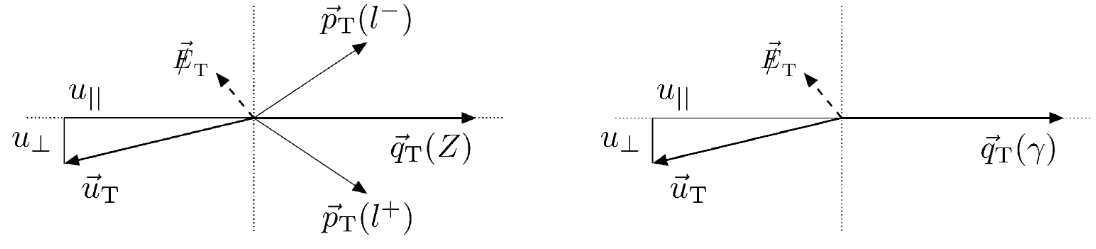
\includegraphics[width=0.95\textwidth]{MET}
\caption{ Z boson (left) and photon (right) kinematics with the vector of all the visible objects (denoted by u) and a resulting MET.}
\label{fig:MET}
\end{figure}


%following the twiki:
%\begin{center}
%\texttt{https://twiki.cern.ch/twiki/bin/viewauth/CMS/MissingETRun2Corrections}
%\end{center}
%On top, a set of filters related to the instrumental effects is employed:
%\begin{center}
%\texttt{https://twiki.cern.ch/twiki/bin/view/CMS/MissingETOptionalFiltersRun2}
%\end{center}

\section{Event Selection}
\label{sec:selection}

%Two analysis methods are pursued to select samples that can be 
%used to extract the signal yield from the data in an optimal way.
The resonances in search decay to two SM Higgs bosons. However, Higgs bosons further decay almost immediately. Therefore, it is critical to reconstruct Higgs bosons decay products with the high precision. 

\subsection{Higgs and Z Boson Selection}



Only dilepton pairs having net charge of zero are considered as \ZtoLL~ candidates. 
Pairs of prompt isolated leptons must have a dilepton mass greater than 76 GeV. This ensures the orthogonality with HIG-17-006 bbVV analysis (later also referred to as bbWW analysis) as well as helps selecting decays of real Z bosons.

Higgs boson candidates are reconstructed from the b jet pairs utilising the two b jets with the highest CMVAv2 discriminant value. We do not veto additional b jets as with the increased PU growths the probability to have more b jets. 

Double Higgs boson candidate is computed as a sum of Lorentz vectors of the \ZtoLL~ candidate, MET, and a \HBB~ candidate. Then, we compute the transverse mass of that object. 

This transverse mass definition that we follow is one of the commonly used and is logical in the sense that we subtract the longitudinal momentum component which leaves us with the transverse momentum components only (while the energy remains the total energy). More precisely, as the z-component of the neutrinos' momentum is unknown and we decided not to reconstruct it, we form a pseudo transverse mass: $\tilde{M}_T(HH) = \sqrt{E^2 - p_{z}^2}$ (further referred as transverse mass for brevity), where $E$ and $p_z$ are the energy and the z-axis component of the Lorentz energy-momentum vector of the HH candidate.

The resulting distribution, $\tilde{M}_T(HH)$, is what will be used in the binned shape analysis with the Higgs Combination Tool following the section "Binned shape analysis" as described at the twiki page~\cite{CombinedLimit}. Shape analysis is more sensitive than the simple cut-and-count experiment (one bin distributions) since more information/discrimination power is given to the likelihood function. 

%:
%\begin{center}
%    \small{\texttt{https://twiki.cern.ch/twiki/bin/view/CMS/SWGuideHiggsAnalysisCombinedLimit}}
%\end{center}
Initial data files, called ntuples, have enormous size of the order of more than a Terabyte per background process. To reduce the size of the ntuples and remove clear background events (on the other hand, to remove signal-like events we apply a sophisticated selection and use a BDT), we apply a "common-sense" HH preselection, which starts with the requirement on dilepton mass to be greater than 50 GeV and the event to contain at least two "good" jets - with $p_{T} > 30$ GeV and $|\eta| < 2.4$. In addition to requirements on Higgs bosons decaying to b quarks mentioned above, we define Z bosons as two opposite sign muons with $p_{T} > 20/15$ GeV (leading/subleading lepton) or two opposite sign electrons with $p_{T} > 25/15$ GeV (leading/subleading lepton). 



Later analysis cuts, the selection chain to improve signal-background separation, include: 

 \begin{itemize}
 \item  the requirement of at least two b jets in the event, out of which two with the highest CMVAv2 score are used to define \HBB ~candidate
 \item  the lower end cut on the \HBB ~mass set to 20 GeV to remove the low mass resonances, while giving BDT as many events in the CRDY as possible at the same time. The upper end cut is not explicitly set for the same purpose. The actual \HBB ~mass distribution after the analysis selection is concentrated in the range 30 to 220 GeV
 \item  the Z boson selection takes the most energetic two leptons of the opposite sign and requires their dilepton mass to pass 76 GeV < Z mass < 106 GeV condition used for the signal region definition. This is a standard $\pm$ 15 GeV window for Z boson selection whose lower end also preserves othogonality with the existing HIG-17-006 bbVV analysis
 \item  HH candidate is approximated by the sum of \ETslash, Z, and \HBB~decays. A loose cut on HH transverse  $>100$ GeV removes evidently background events
 \item  finally, an additional set of \ETslash cuts is used to ensure orthogonality with the existing HIG-18-013 bbZZ analysis focusing on the 2b jets + 2 leptons + 2 quarks, see Table \ref{metCuts}. The MET cuts have been optimised by both analyses to yield the best limit when the results of two measurements are combined. 
 \end{itemize}


\begin{table}[H]
\begin{center}
\caption{\ETslash cut to orthogonalise the analysis with respect to HIG-18-013.}
\begin{tabular}{|c|c|} \hline
{Signal mass, GeV} &  \ETslash cut, GeV\\\hline
260-300     &                                \textgreater~40 \\
350-600     &                                \textgreater~75 \\
650-1000    &                                \textgreater~100 \\
\hline
\end{tabular}
\label{metCuts}
\end{center}
\end{table}


\begin{figure}[H]%hbpt?                                                                       
  \begin{center}
    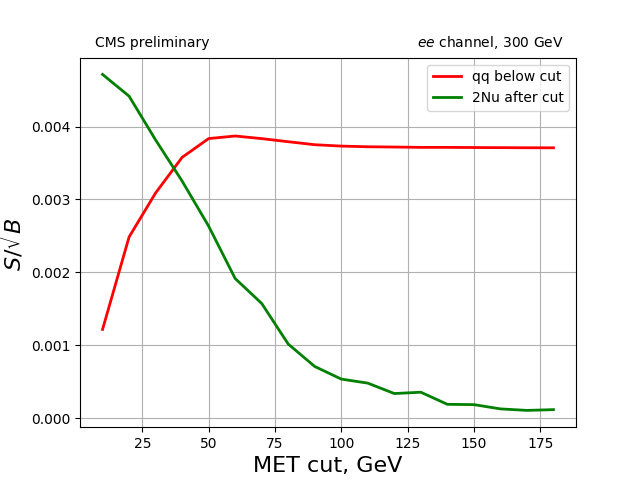
\includegraphics[width=0.45\textwidth]{ee_300_met.png}
    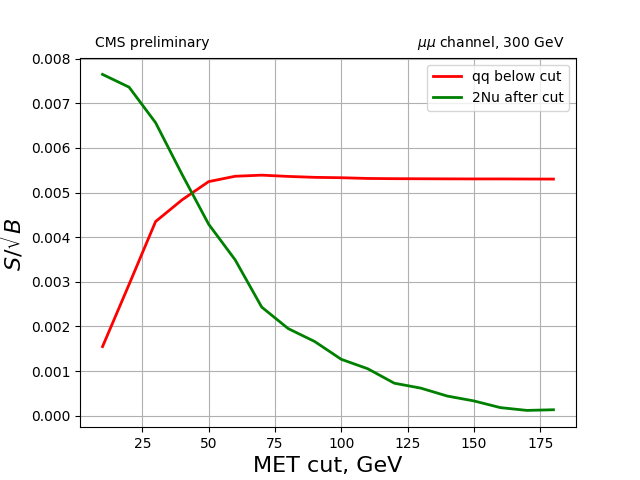
\includegraphics[width=0.45\textwidth]{mm_300_met.png}\\
    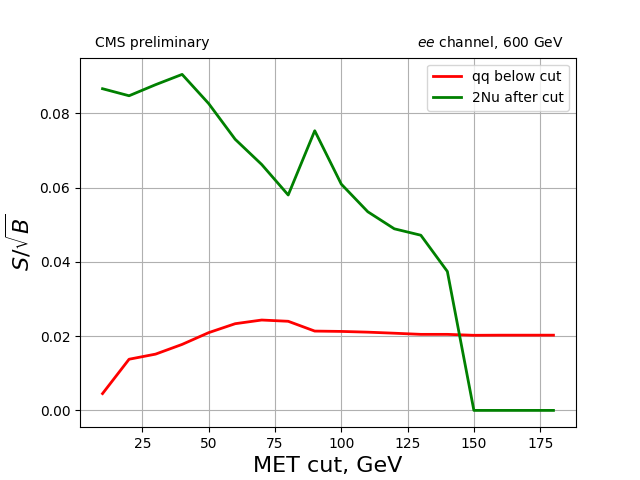
\includegraphics[width=0.45\textwidth]{ee_600_met.png}
    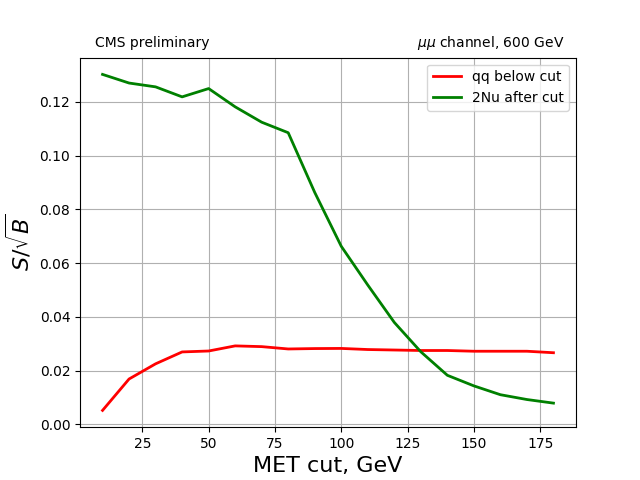
\includegraphics[width=0.45\textwidth]{mm_600_met.png}\\
    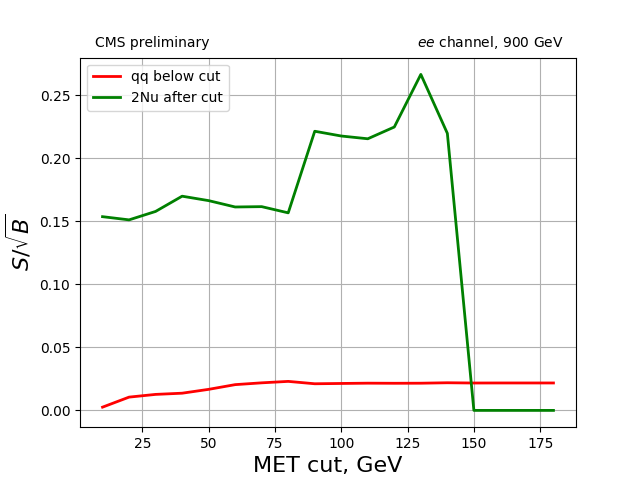
\includegraphics[width=0.45\textwidth]{ee_900_met.png}
    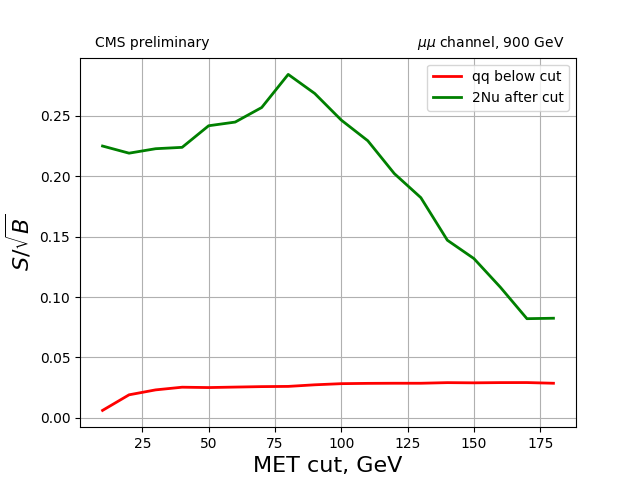
\includegraphics[width=0.45\textwidth]{mm_900_met.png}\\
    \caption{ Significance-like ($\sqrt{S}/B$) figure of merit as a function of the MET cut. Green curve shows the significance for our analysis keepings event above the cut, red curve is for HIG-18-013 analysis and their phase space is below the cut value. Top: 300 GeV cut. Middle: 600 GeV cut. Bottom: 900 GeV cut. On the left dielectron channel is shown, while dimuon plots are on the right. }
    \label{fig:met_cuts}
  \end{center}
\end{figure}




\subsection{\HBB ~and \ZtoLL ~variables to define signal and control regions}

In this analysis we define three regions in the \HBB ~and \ZtoLL
~space. Two regions, CRDY and CRTT, are used to extract the
normalizations of DY and \ttbar backgrounds correspondingly. Signal region (Fig. ~\ref{fig:regions}) is chosen by
the set of \HBB~and \ZtoLL ~cuts \ref{fig:regions}. To further reduce background contamination in this region, an additional cut on the MVA output is used. Boosted decision trees (BDT) MVA technique is employed to
separate background from signal. Below we describe in details
selection of each region and BDT construction. 

%% Skimming is applied
%% before building BDT to remove unnecessary background, while still
%% keeping a lot of events for BDT training. The set of "HH loose
%% common-sense" \label{hhSelection} skimming/preselection cuts includes: Dilepton (ee/mm)
%% mass $>$ 50 GeV, 2 or more jets: pt $>$ 30 GeV and $|\eta| < 2.4GeV$. Then, we
%% select two or more b-jets, \HBB~ mass should be greater than 20 GeV,
%% exactly two leptons, dilepton mass higher than 76 GeV, transverse mass
%% of HH higher than 100 GeV. The definition of the signal and control regions is illustrated in Fig. \ref{fig:regions}. The signal region is selected in the range of
%% 76 $<$ \mll~ $<$ 106 GeV and %75 $<$ \mbb~ $<$ 175 GeV. This corresponds to the
%% 90 $<$ \mbb~ $<$ 150 GeV. This corresponds to the
%% Z mass +- 15 GeV window. OA
For CRDY we invert \HBB ~cut, keeping in the lower sideband only events
with the mass of Higgs boson higher than 20 GeV to avoid fakes from
QCD. For CRTT we invert \ZtoLL ~cut, keeping only high mass sideband to
ensure the orthogonality with the existing HIG-17-006 bbVV analysis, since the lower sideband is already included in the phase space used by them. 


\begin{figure}[!htb]%hbpt?                                                                       
  \begin{center}
    %\raisebox{0.17\height}                                                                     
    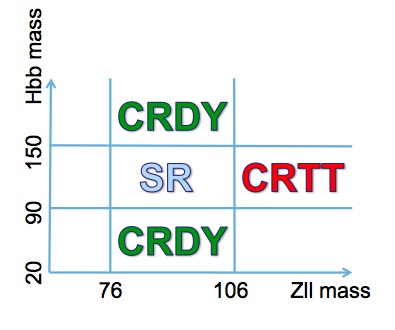
\includegraphics[width=0.45\textwidth]{regions.png}
    \caption{ Signal region, control region \ttbar, and control region Drell-Yan in the phase space of \ZtoLL \ ~and ~\HBB ~masses.    }
    \label{fig:regions}
  \end{center}
\end{figure}


%% \begin{table}
%% \begin{center}
%% \caption{Efficiency of the BDT selection requirement. Dielectron channel. Left: 300 GeV signal mass hypothesis. Right: 900 GeV case.}
%% \begin{tabular}{|c|c|c|} \hline
%% {Process} &  Efficiency at 300 GeV, \% &  Efficiency at 900 GeV, \% \\\hline

%% signal (bbZZ) &                       85 &                       86 \\
%% signal (bbWW) &                       60 &                       82 \\
%% \ttbar        &                       28 &                       $\sim$ 0 \\
%% Drell-Yan     &                       64 &                       $\sim$ 0 \\
%% Single top    &                       33 &                        1 \\
%% ZH            &                       76 &                        4 \\
%% Dibosons      &                       76 &                        2 \\\hline

%% \end{tabular}
%% \label{EfficiencyBDT}
%% \end{center}
%% \end{table}


\begin{table}                                                                                                                                                                          
\begin{center}      
                                                                                                                                                                   
\caption{Efficiency of the BDT selection requirement. $ee$ channel (top) and $\mu\mu$ channel (bottom). }
\begin{tabular}{|c|c|c|}
\hline
sample & Efficiency at 300 GeV, [\%] &  Efficiency at 900 GeV, [\%] \\
\hline
signal (bbZZ) &                        89.2 &                        94.9 \\
signal (bbWW) &                        75.0 &                        88.4 \\
\ttbar        &                        28.8 &                         0.2 \\
Drell-Yan     &                        74.2 &                         1.2 \\
Single top    &                        33.1 &                         1.1 \\
ZH            &                        88.8 &                        10.7 \\
Dibosons      &                        90.0 &                         5.0 \\
\hline
\end{tabular}
%\vspace*{1cm}
\begin{tabular}{|c|c|c|}
\hline
sample &  Efficiency at 300 GeV, [\%] &  Efficiency at 900 GeV, [\%] \\
\hline
signal (bbZZ) &                        58.1 &                        91.1 \\
signal (bbWW) &                        25.9 &                        96.3 \\
\ttbar        &                        13.6 &                         0.2 \\
Drell-Yan     &                        39.0 &                         0.8 \\
Single top    &                        13.0 &                         0.2 \\
ZH            &                        56.0 &                         8.4 \\
Dibosons      &                        51.4 &                         6.2 \\
\hline
\end{tabular}

\label{EfficiencyBDT}                                                                                                                                                                  
\end{center}                                                                                                                                                                           
\end{table} 


%
%
%\begin{figure}[tbp]
%  \begin{center}
%    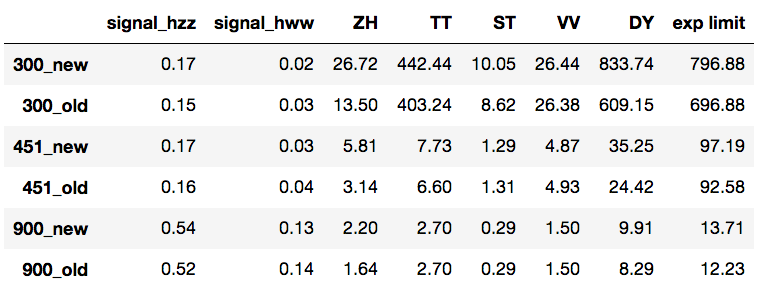
\includegraphics[width=0.91\textwidth]{ee_yields.png}
%    \caption{Yields for ee channel before and after the tight isolation bug fix in the HEPPY. The effect is minimal as can be seen in the final limit. }
%    \label{fig:yields_ee}
%  \end{center}
%\end{figure}
%


\section{Signal and background characteristics}

The signal region is further purified removing backgrounds by applying the cut on the BDT
output (Table ~\ref{EfficiencyBDT} contains the efficiency numbers for the BDT cut). 
The first set of BDT variables in the early version of the analysis included 30-50 variables, which could potentially discriminate signal from the background. The set contained variables related to the kinematic properties of the signature, as well as a dozen of angular variables. After the first optimization of the BDT training and produced ranking of variables, nine best variables were determined and chosen to be used for the final analysis. Removal or addition of other variables did not improve the performance significantly. To simplify the analysis, the same set of nine variables is used in both low and high mass trainings and for both spin hypotheses.

With 16 masses points in the range from 250 to 1000 GeV, one can: train 16 discriminants, train one complex hyperparametrised neural network, split the mass range into regions with the similar kinematics and thus train only few BDTs. The latter is the approach that has been adopted by mature (legacy) HH analyses, and we are following the same procedure. We split the mass range into two: low mass and high mass (\`a la HIG-17-002 and HIG-17-008). These simplification costs some performance loss but allows analysis to proceed with just two BDTs instead of training one BDT per mass point, which would require more than a dozen of trainings per heavy resonance. In case of the infinite statistics, training a dedicated BDT for each
signal mass hypothesis would give a better performance, but in our case we are statistics dominated, thus training only two BDTs also has benefits in terms of the size of the signal sample, absence of the overtraining etc. In addition, the adopted path saves computational resources. Lastly, physics-wise, bbZZ signature is not the most sensitive, bb$\gamma$$\gamma$ is due to an excellent CMS diphoton mass resolution. Thus, the difference in sensitivity is a factor of 30-100 depending on the mass. Therefore, training a dozen of BDTs is clearly impractical. For more discussion on the topic please refer to the chapter \ref{sec:BDT}.





%In addition, it would require a training of 16 BDTs per particle (BulkGraviton in our case). 
The low/high mass boundary value for HH analyses is chosen typically in the range 300-450
GeV. In our case the performance of the boundary around 300 GeV (area under the ROC curve
for low mass BDT is 0.9138 and 0.9805 for high mass BDT) is
similar to the boundary option at the 450 GeV (area under the ROC curve
for low mass BDT is 0.9086 and 0.9957 for high mass BDT), and to the one in the
middle of the range (area under the ROC curve
for 400 GeV for low mass BDT is 0.9074 and 0.9928 for high mass BDT). 
%https://indico.cern.ch/event/628835/contributions/2639777/attachments/1483653/2302207/Rami_HH_27June2017_v3.pdf
Therefore, we chose the value of 450 GeV, which
is also a choice of the bbbb analysis \cite{bbbb}. Upon running the full analysis chain up to the expected limits, the choice of 450 GeV was verified to be the best split point option: the usage of the high mass BDT at the 400 GeV or low mass BDT at the 500 GeV was yielding suboptimal results thus confirming the mass boundary choice. 

Splitting the mass range into two regions, we arrive at the low
mass BDT, which merges (with the weight '1') seven signal samples:
250, 260, 270, 300, 350 400, 450 GeV, and the high mass BDT, which combines nine signal samples of 
masses: 500, 550, 600, 650, 700, 750, 800, 900, 1000. In each case the
composition of the background is the same, it is a mix (by cross
section) of \ttbar and Drell-Yan plus jets.


Cut flow for $ee$ and $\mu\mu$ channels from the generator level up to before the BDT selection is shown on the figures ~\ref{fig:cutFlow}. In the cut flow table ~\ref{fig:cutFlow} the following definitions are used: very loose selection means all GsfElectrons and Muons from the basic collections that match generator level electrons/muons and pass the very minimal kinematic cuts; loose selection means loose POG selection consisting of kinematic cuts, impact parameters dxy and dz, and iso cuts. Shown final efficiency values are given in terms of the number of events ~\ref{cutFlowEvents}:

\begin{table}
\begin{center}
\caption{Number of events surviving analysis cuts corresponding to the last entry in the ~\ref{fig:cutFlow} .}
\begin{tabular}{|c|c|c|} \hline
{Process, mass point} &  ee channel, \% &  mm channel, \% \\\hline
bbZZ, 300 GeV &                    2256     &                    4511 \\
bbWW, 300 GeV &                    53       &                    85 \\
bbZZ, 900 GeV &                    8034     &                    12963 \\
bbWW, 900 GeV &                    12       &                    23 \\\hline
\end{tabular}
\label{cutFlowEvents}
\end{center}
\end{table}



\subsection{Data and MC comparison\label{sec:compareDataMC}}
%Signal region BDT sideband plots as well as unblind signal region plots show good data-MC agreements.
BDT selection is applied in the signal region only, we are not cutting on BDT for control regions, therefore, all the mass
points belonging to the low mass region (and separately to the high mass region) have the same background and data distributions. Thus, we provide plots for two mass points: one mass point representing low mass region, 300 GeV, and one mass point representing high mass region, 900 GeV. 
% for other pass point only signal distribution will change,
%however, data/background comparison and their ratio will not. At the same time, BDT outputs are mass point specific, because are trained for two different mass regions - low and high mass regions, and are evaluated for each mass point separately. Thus, we show all the BDT plots. 
Signal bbZZ and bbWW rates for all plots are multiplied additionally by a factor of 500 purely for the visualization purpose and do not go in the real analysis. 

%Prefit plots are available in the Appendix ~\ref{sec:datamc}. Control regions only postfit plots have been produced during an extensive discussion with Higgs conveners at HyperNews, and it was shows that upon inclusion of the SR in the fit the data-MC agreement is slightly better. 

Postfit plots that include SR in the simultaneous fit with control regions, hence a common jargon name "Full postfit" plots, in contrast to the control regions only type of the fit, or a control regions plus signal region sideband. Figures ~\ref{fig:MCcomparisons} - ~\ref{fig:MCcomparisons_radion} show data and MC comparison in the SR, CRDY, and CRTT. For both $ee$ and $\mu\mu$ channels, low and high mass regions. The latest style plots produced for the analysis public document (Physics Analysis Summary called "PAS") can be found at Fig.~\ref{fig:MCcomparisons} for the graviton case and Fig.~\ref{fig:MCcomparisons_radion} for the radion case. 


%%%%%%%%%%%%%%%%%%%%%%%%%%%%%%%%%%%
%%%%%%%%%%%%%%%%%%%%%%%%%%%%%%%%%%%

Distributions of nine variables that go into the BDT have been studied in depth during the pre-approval process and are available in the Appendix of the analysis note ~\cite{bbZZAN}. All variables show good data/MC agreement after applying postfit scale factors (not to be confused with the POG recommended scale factors in the section below). %After the tight isolation cut fix in the HEPPY framework the results/shapes are almost unchanged (it is also can be observed from the table of yields ~\ref{fig:yields_ee}).  At the yields table ~\ref{fig:yields_ee}, 450 GeV mass point, since evaluated using the high mass BDT, is called 451 GeV for clarity purposes. 
The most important variables in this analysis, namely the BDT itself and the variable that we fit, \mTHH, are shown in the Fig.~\ref{fig:MCcomparisons} for graviton and in Fig.~\ref{fig:MCcomparisons_radion} for the radion. 


\begin{figure}[tbp]
  \begin{center}
    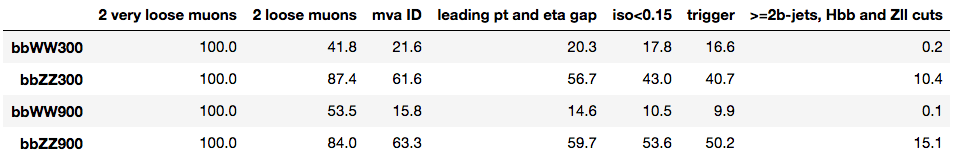
\includegraphics[width=0.91\textwidth]{cutflow_mm.png}\\
    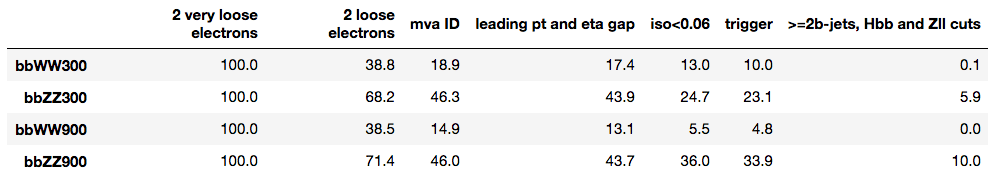
\includegraphics[width=0.91\textwidth]{cutflow_ee.png}\\
    \caption{Cut flow for mm (top) and ee (bottom) channels. }
    \label{fig:cutFlow}
  \end{center}
\end{figure}


                                                                                                                                            

\begin{figure}[tbp]
  \begin{center}
    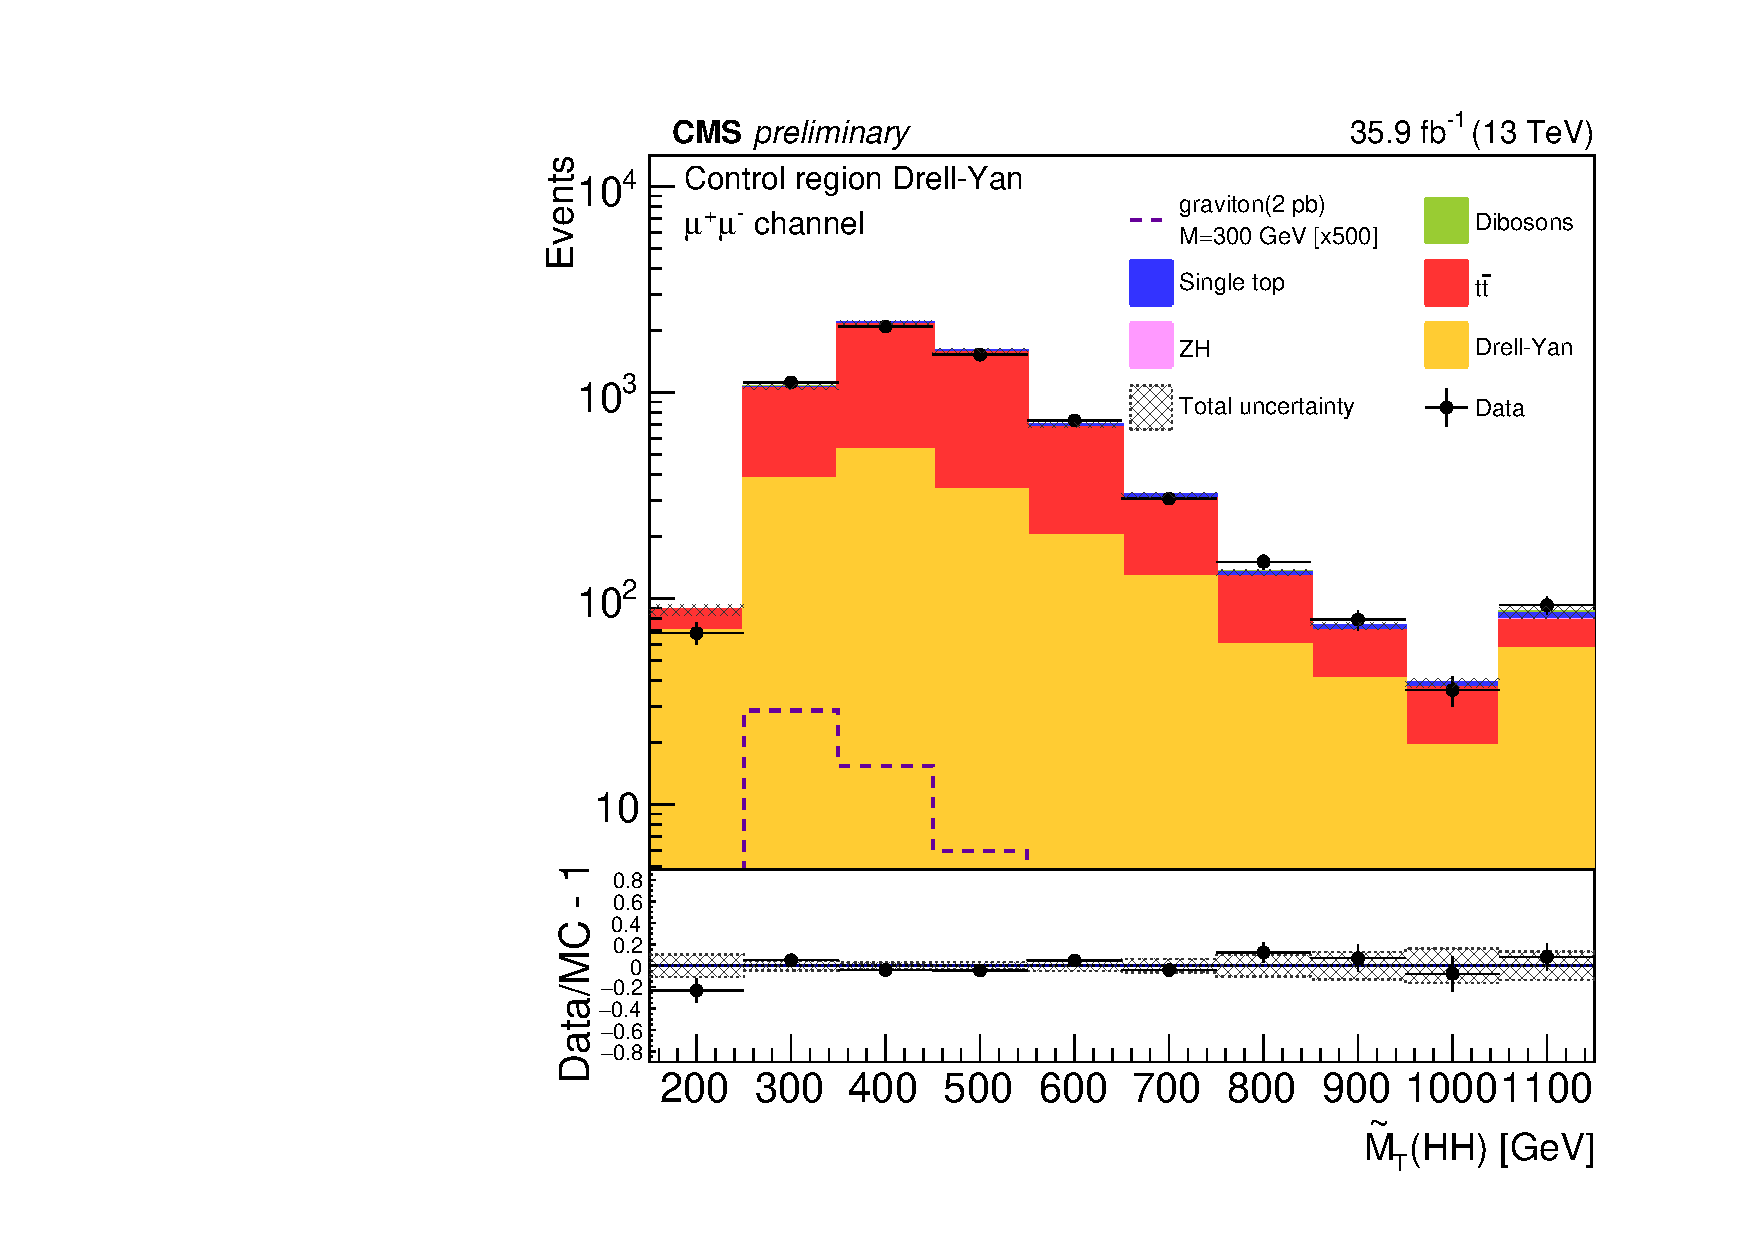
\includegraphics[width=0.31\textwidth]{hhMt_mm_CRDY_FullPostfit_plot_nov16_2_graviton.pdf}
    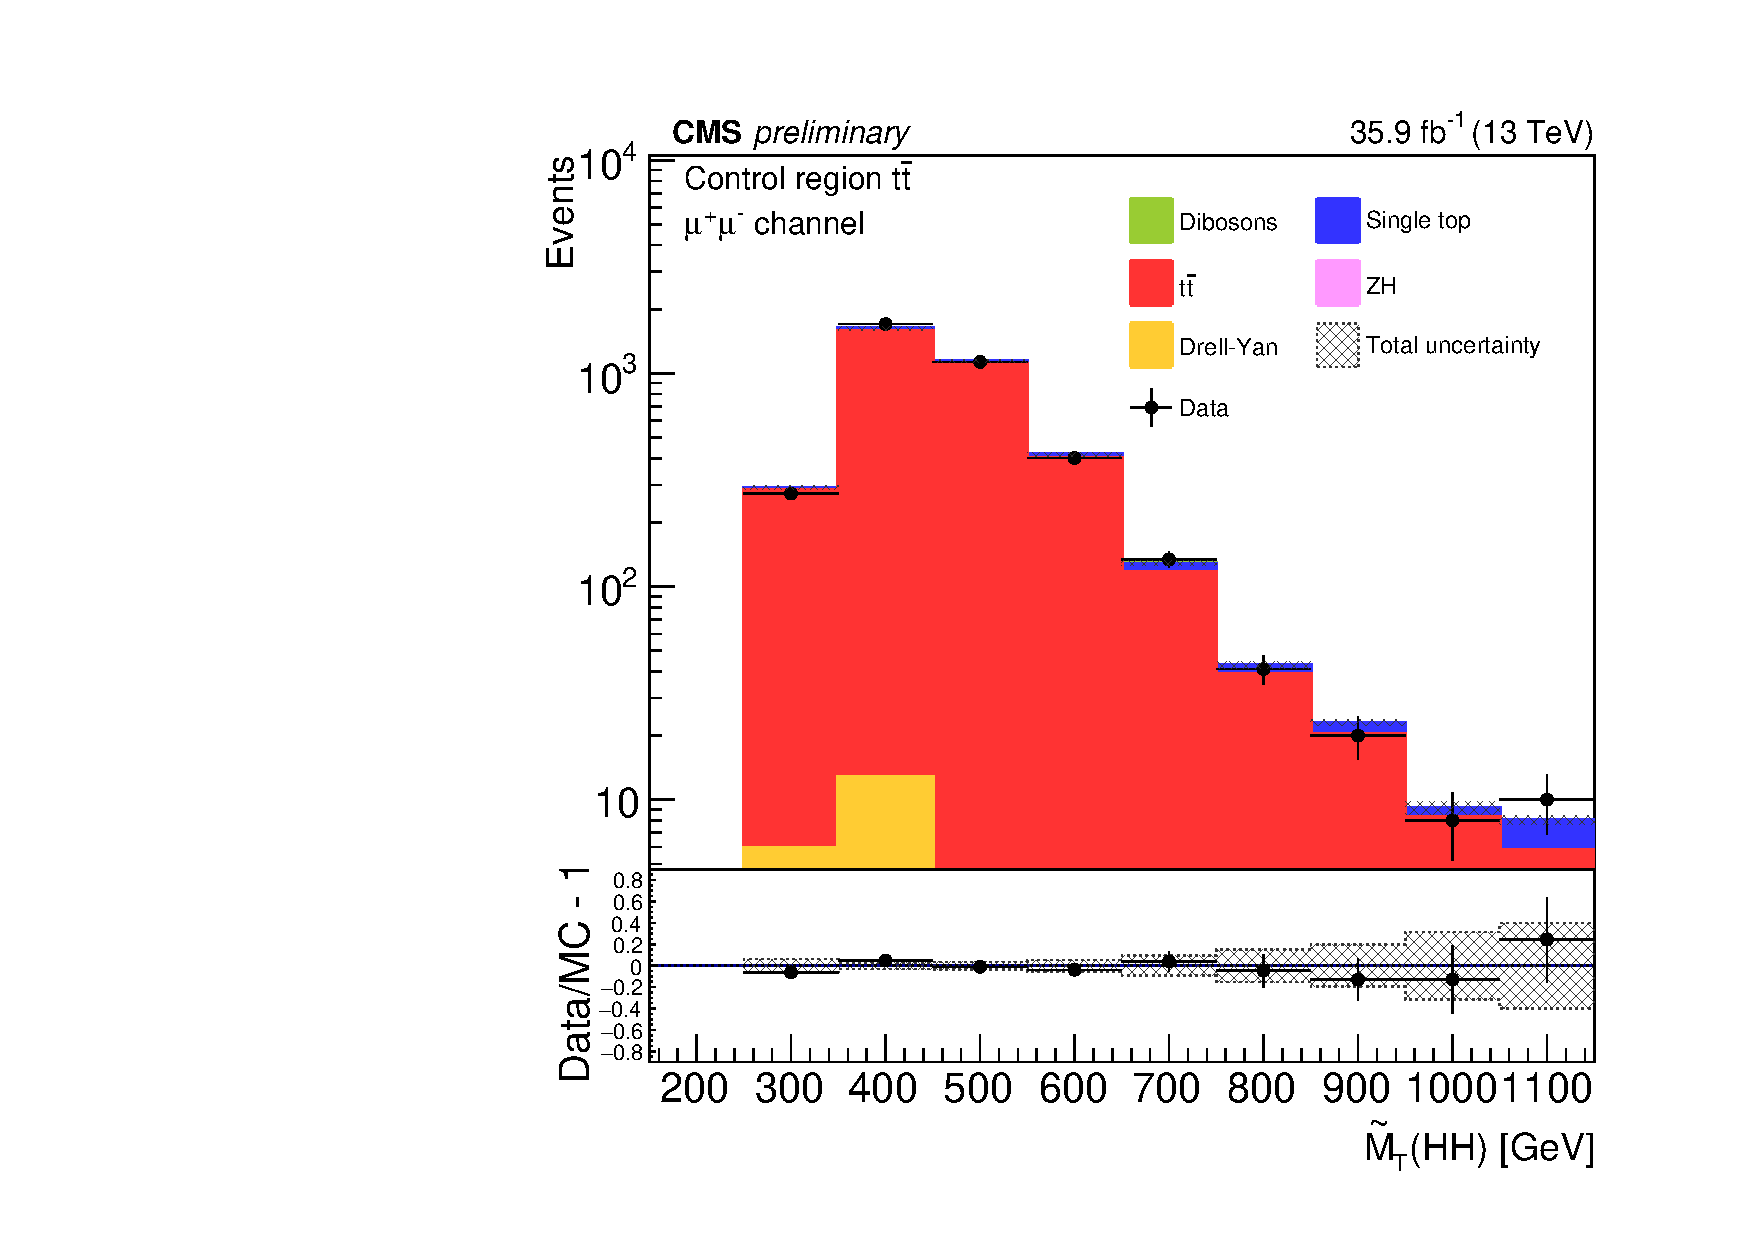
\includegraphics[width=0.31\textwidth]{hhMt_mm_CRTT_FullPostfit_plot_nov16_2_graviton.pdf}
    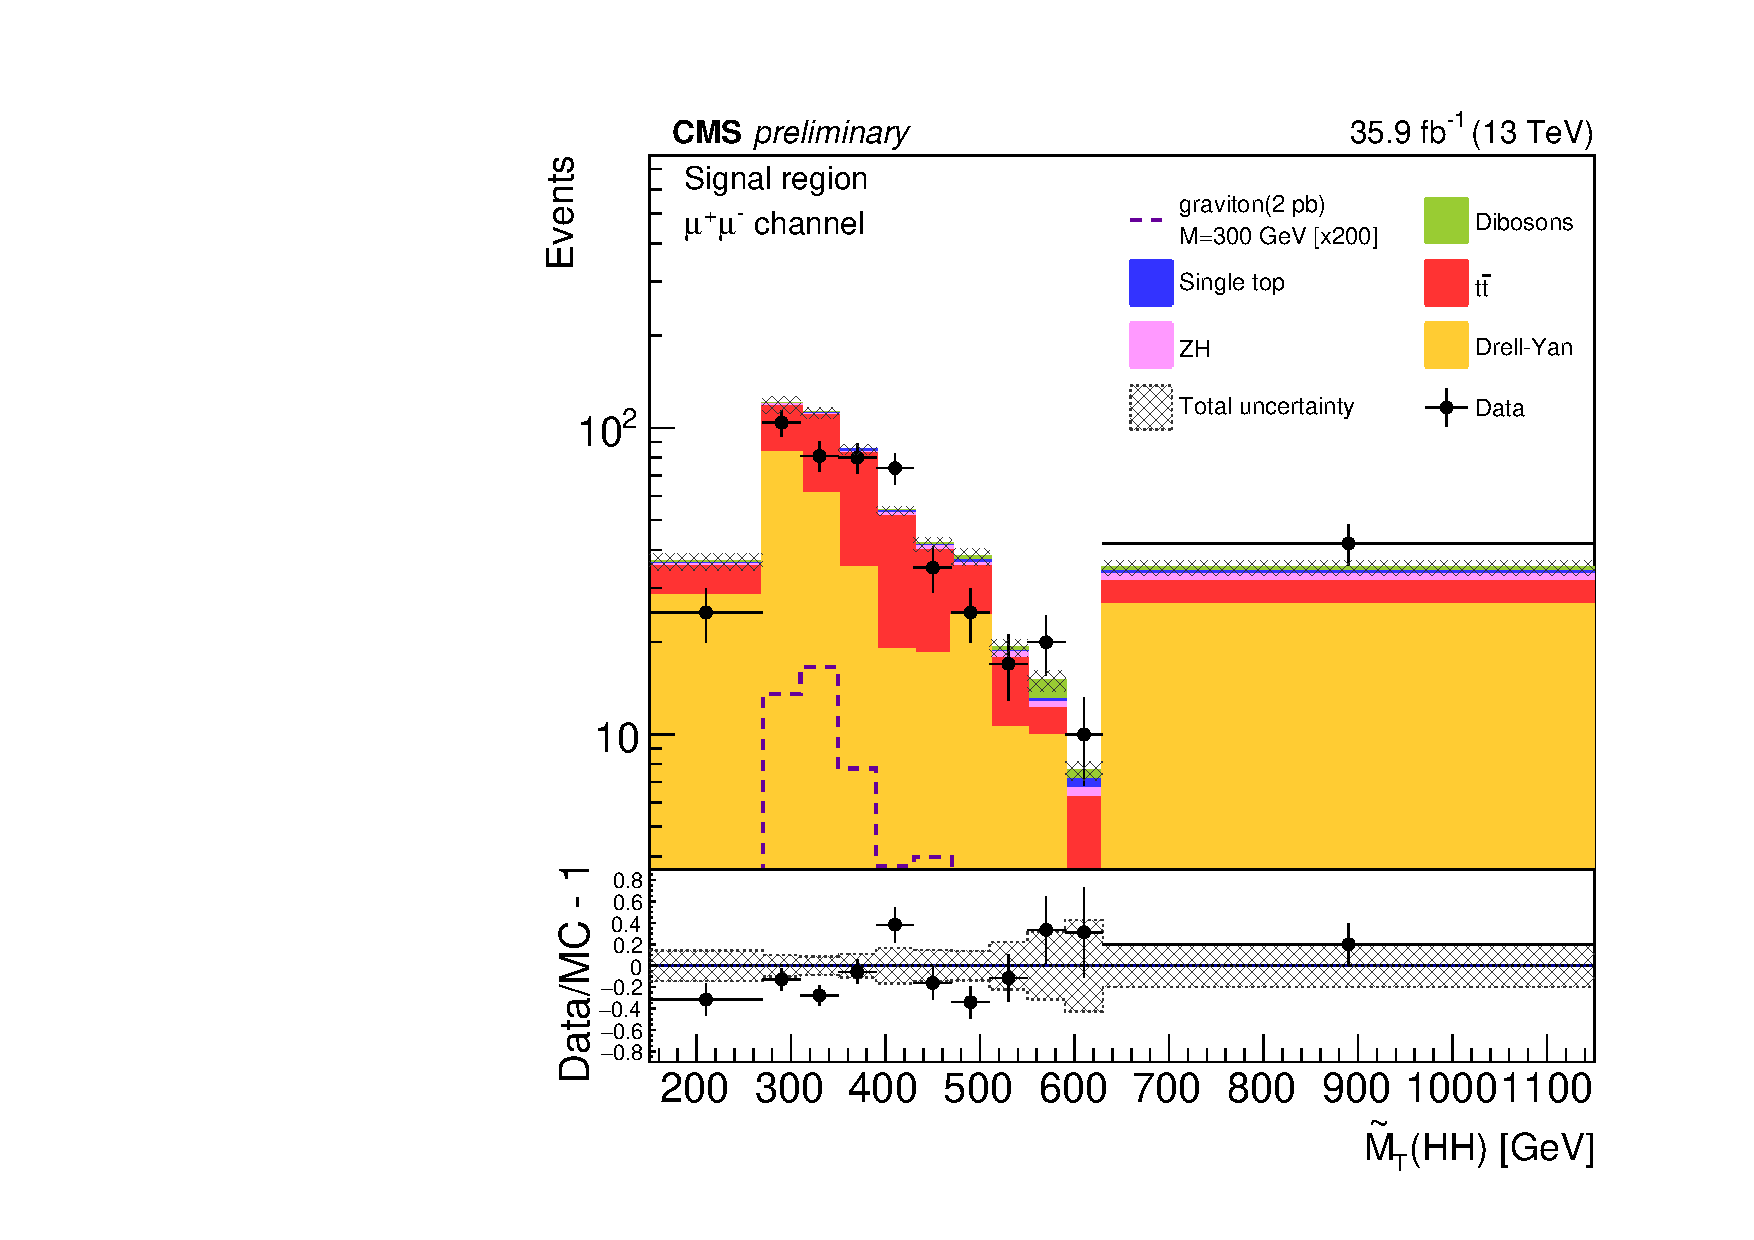
\includegraphics[width=0.31\textwidth]{hhMt_mm_SR_FullPostfit_plot_nov16_2_graviton.pdf} \\
    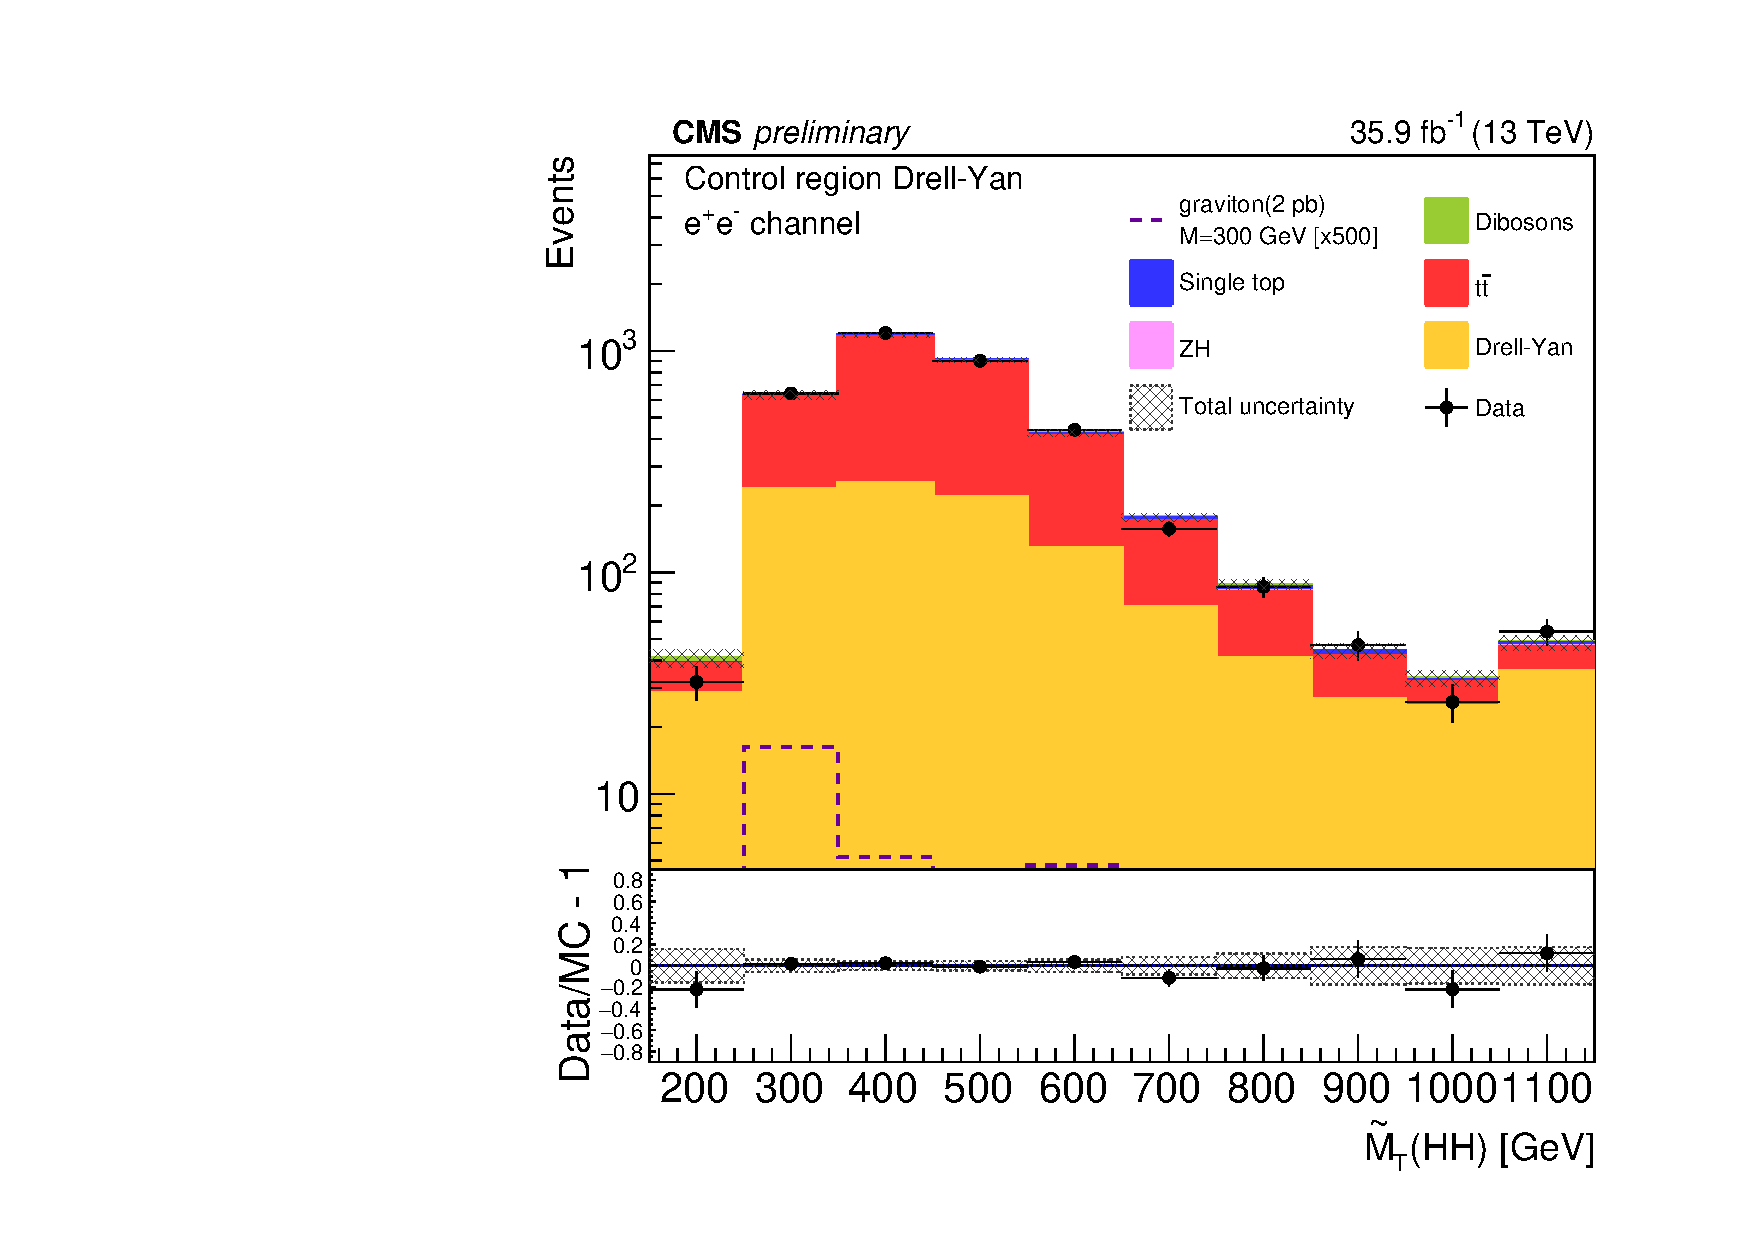
\includegraphics[width=0.31\textwidth]{hhMt_ee_CRDY_FullPostfit_plot_nov16_2_graviton.pdf}
    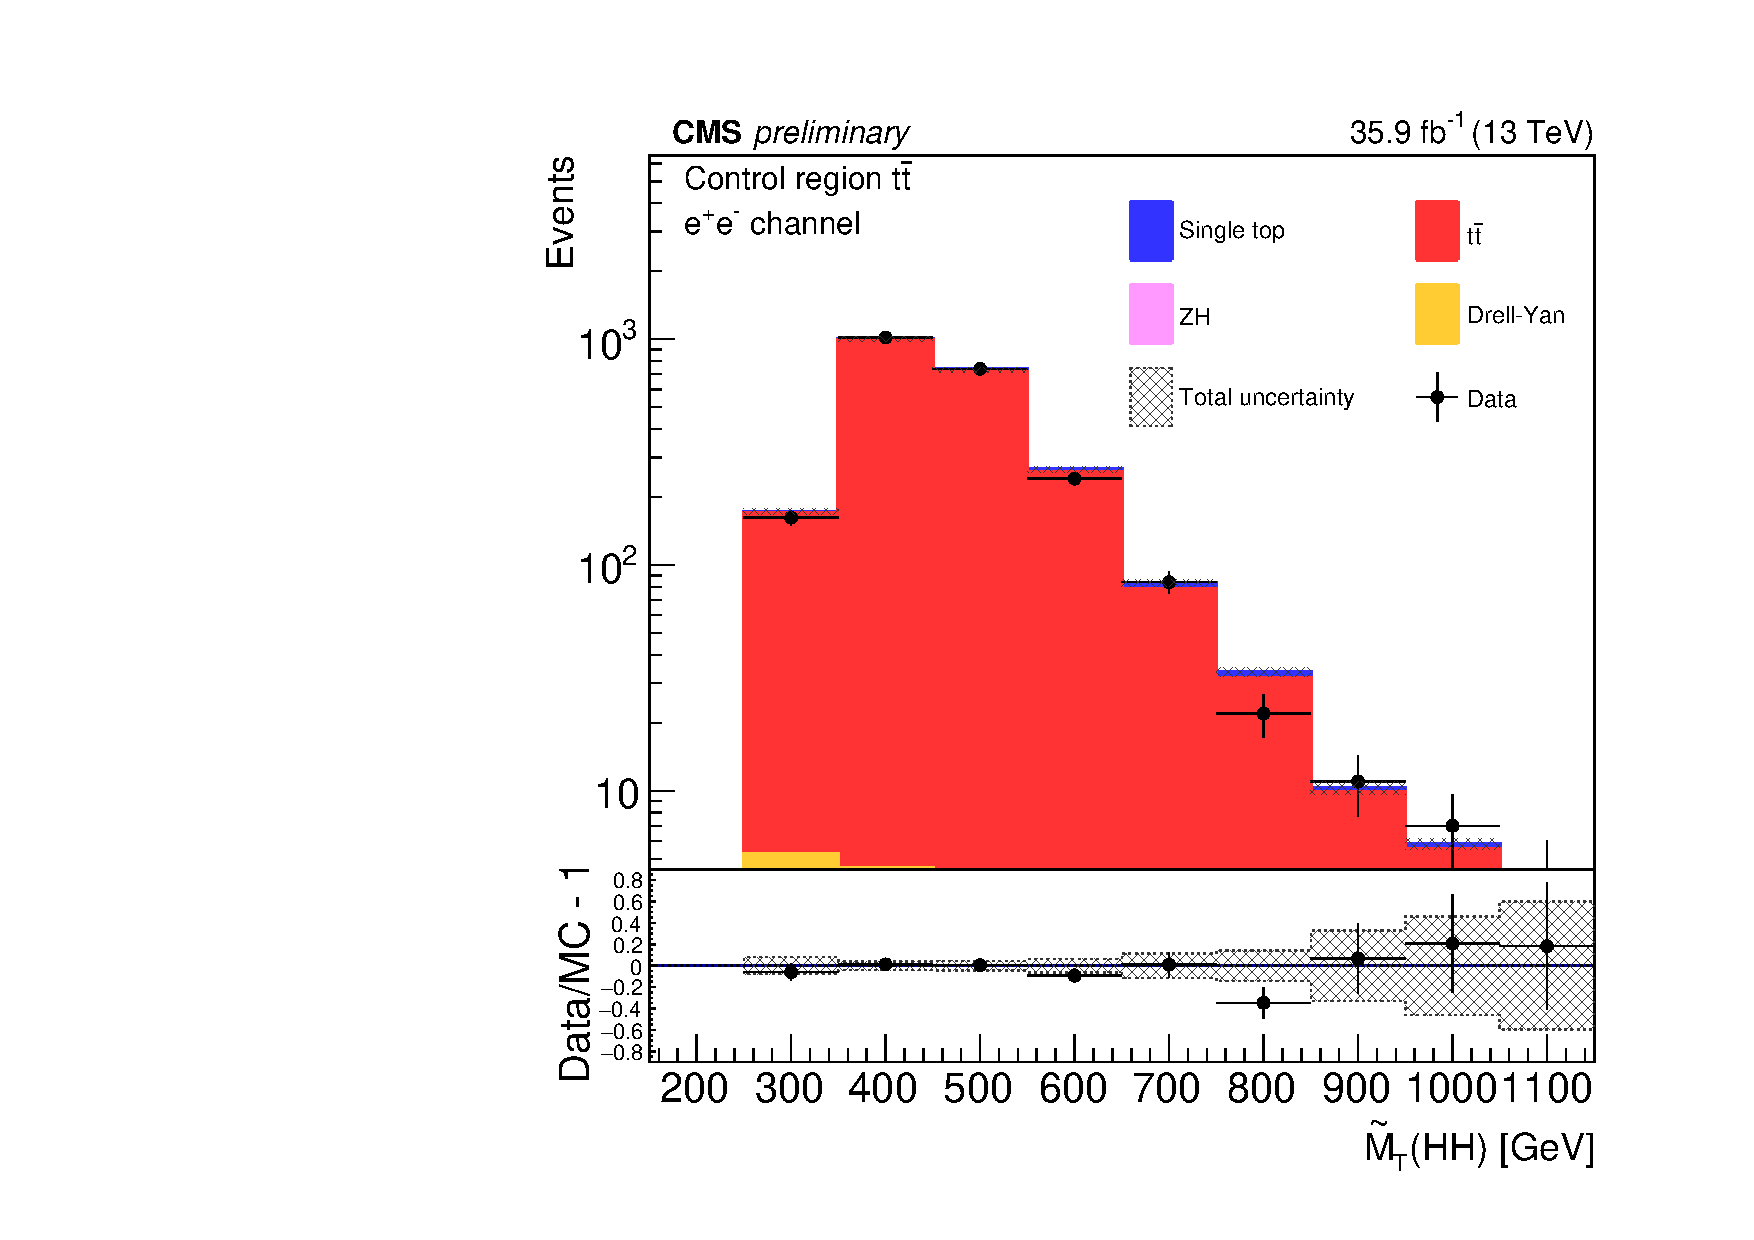
\includegraphics[width=0.31\textwidth]{hhMt_ee_CRTT_FullPostfit_plot_nov16_2_graviton.pdf}
    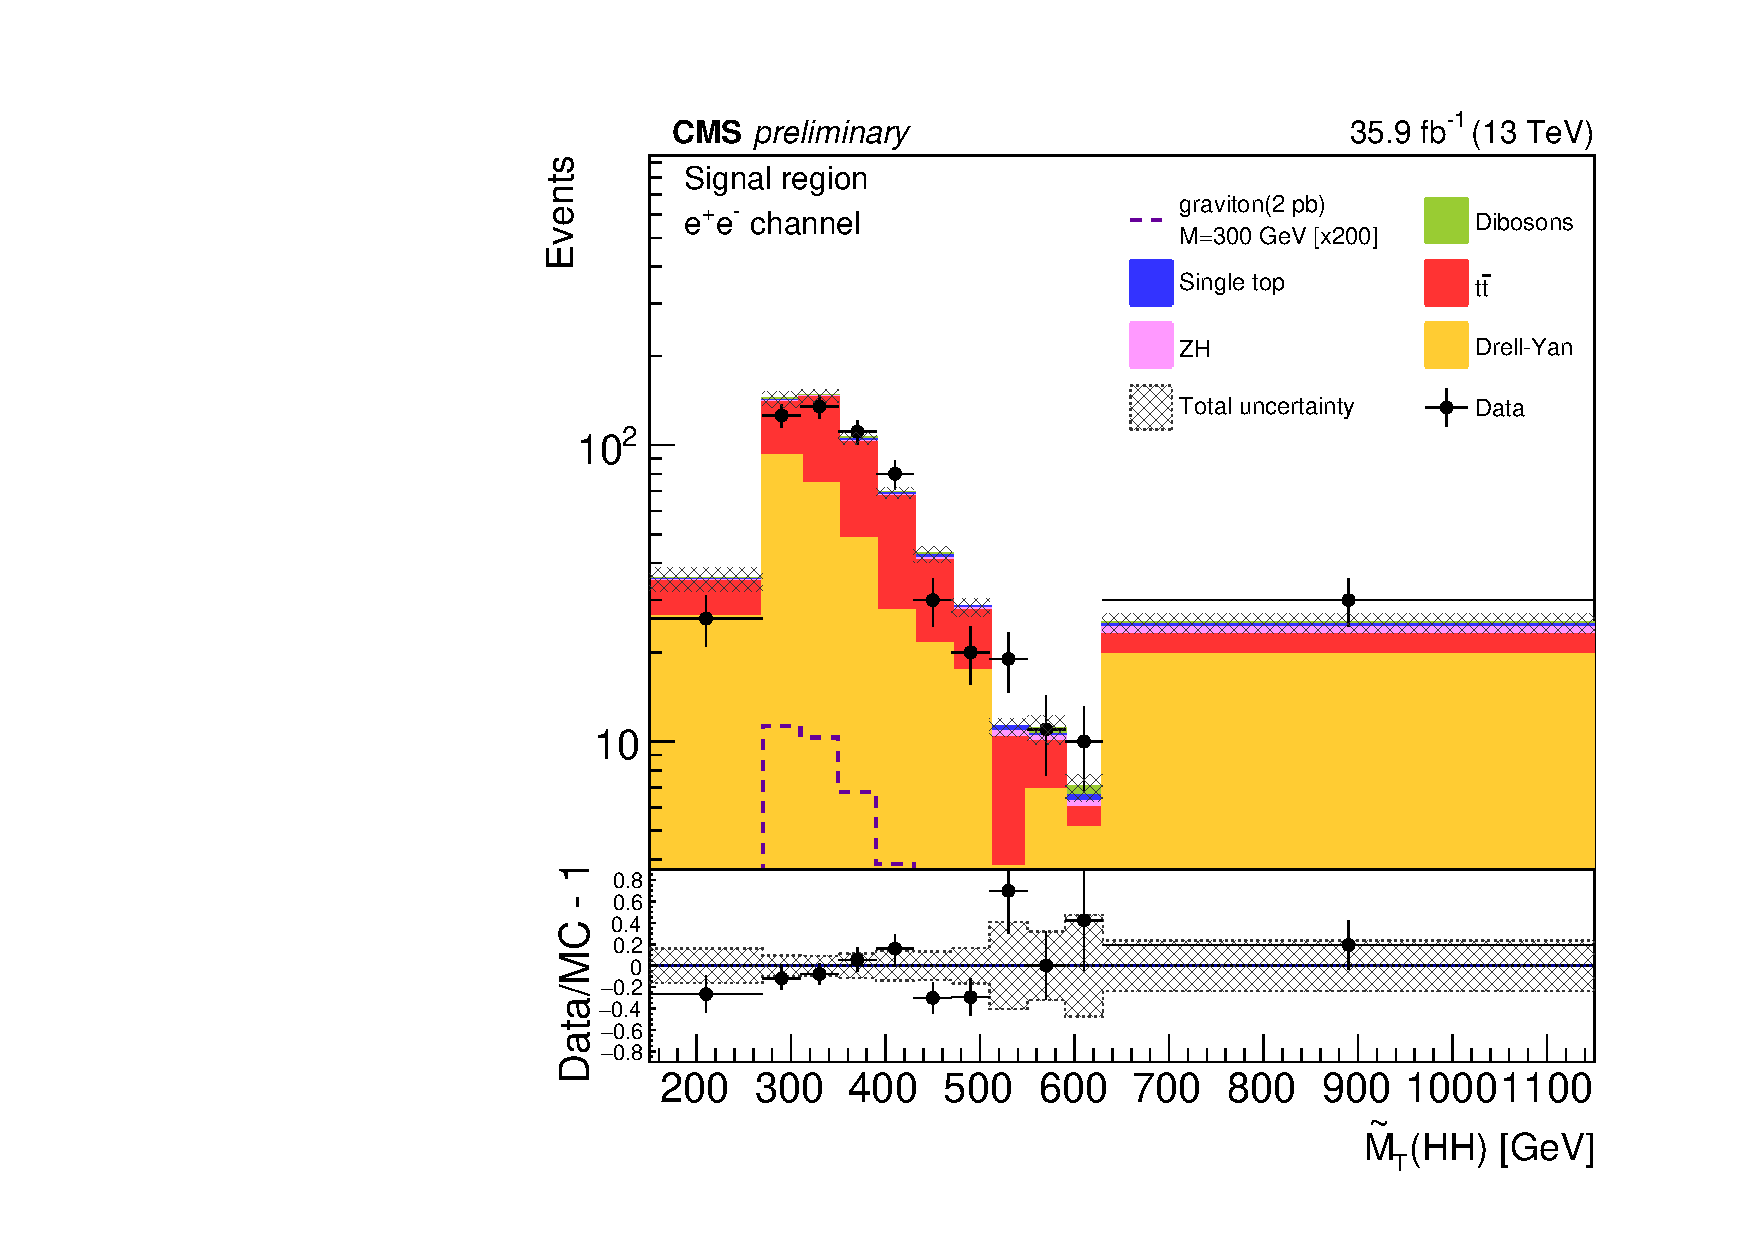
\includegraphics[width=0.31\textwidth]{hhMt_ee_SR_FullPostfit_plot_nov16_2_graviton.pdf}
    \caption{Transverse mass of the reconstructed HH candidates for data, the simulated signal graviton sample
    for the 300 GeV mass hypothesis, and simulated backgrounds scaled according to the fit results. The top
    row shows the figures for the muon channel while the bottom row is for the electron channel. For each row,
    the left plot is for the Drell-Yan control region, the middle is for the \ttbar control region, and the right
    is for the signal region. Signal normalization choice is discussed in the text. The crosshatched area represents
    the sum of statistical and systematic uncertainties.}
    \label{fig:MCcomparisons}
%                                                                                                                 
% Comparison of data and simulation.  Transverse mass of                                                          
%      the reconstructed HH candidate for 300 GeV signal mass                                                     
%      hypothesis, electron channel. Left: Drell-Yan control region. Middle: \ttbar                               
%      control region. Right: signal region. }                                                                    
%    \label{MCcomparisons_electrons}                                                                              
  \end{center}
\end{figure}




\begin{figure}[tbp]
  \begin{center}
    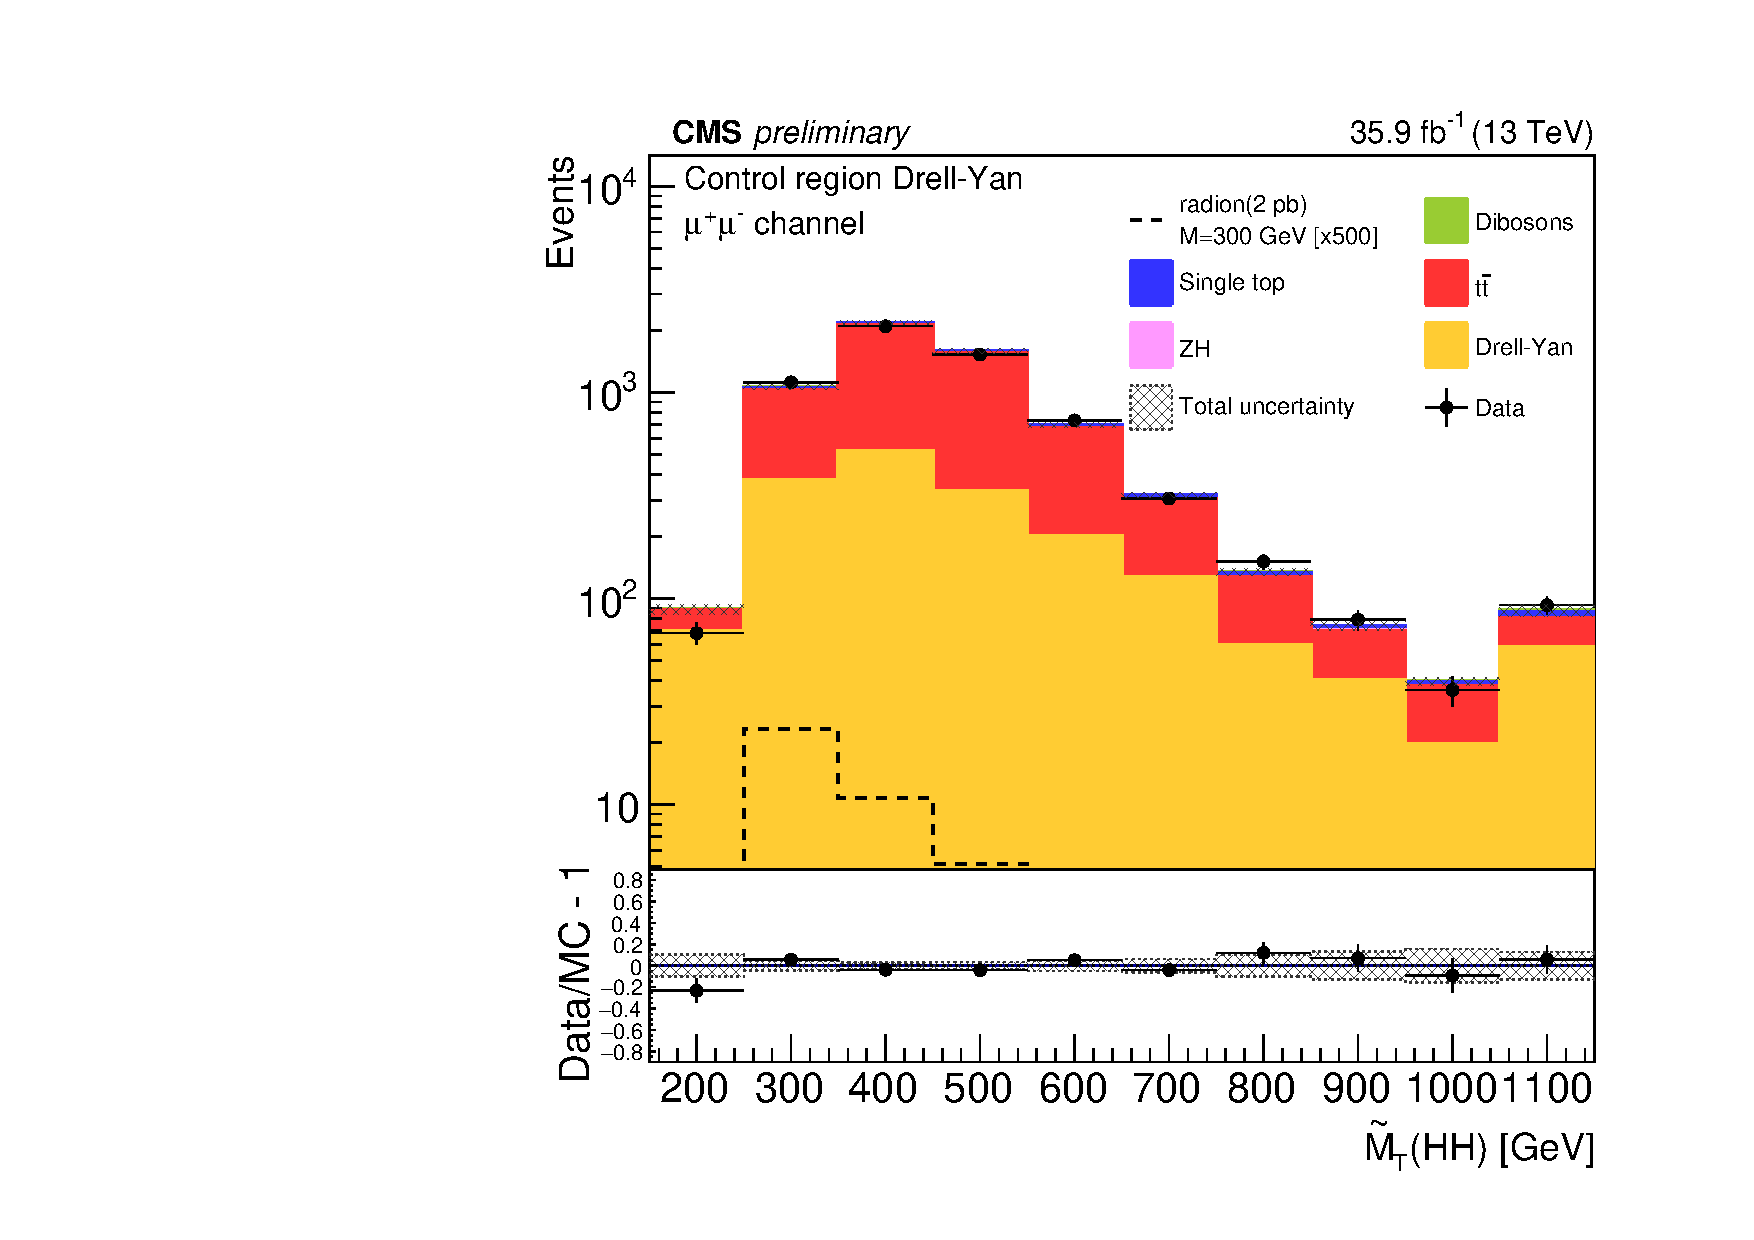
\includegraphics[width=0.31\textwidth]{hhMt_mm_CRDY_FullPostfit_plot_nov16_2_radion.pdf}
    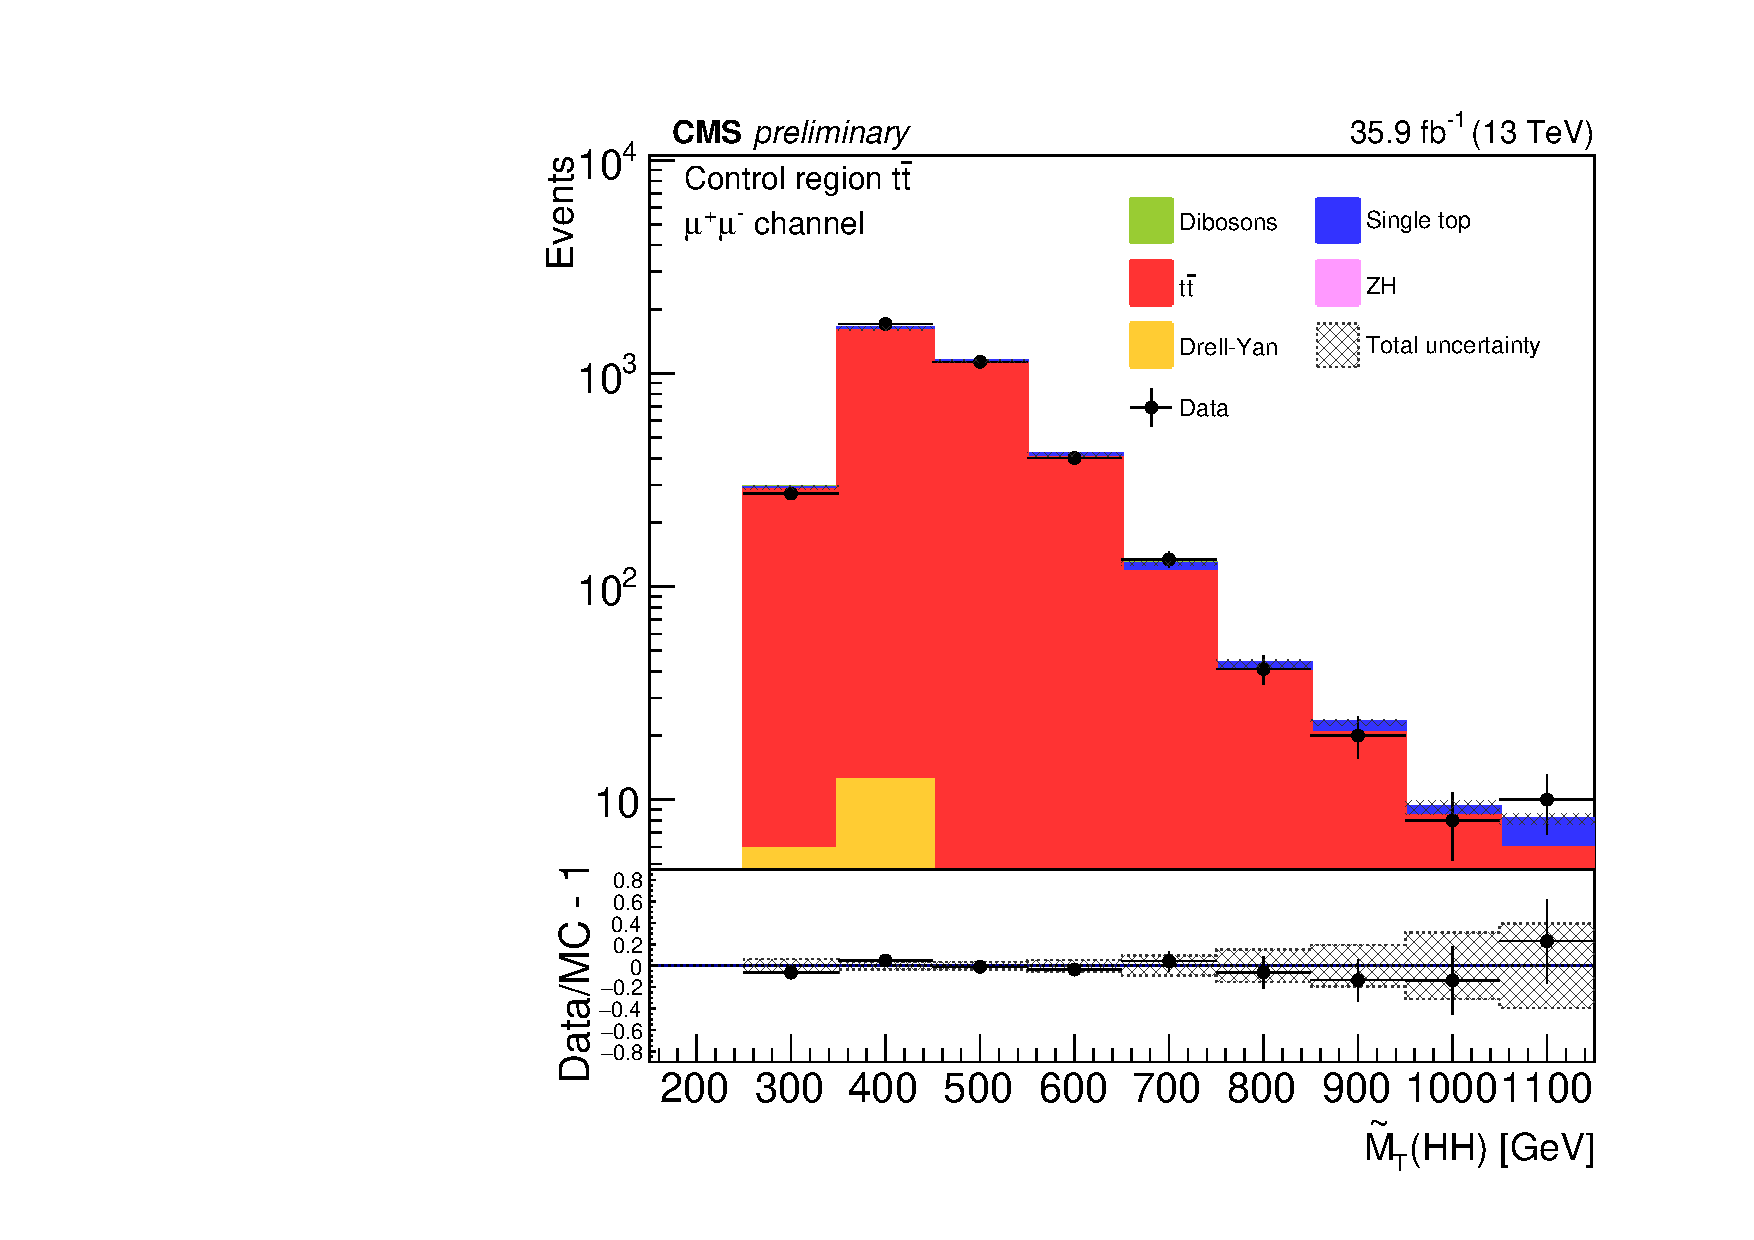
\includegraphics[width=0.31\textwidth]{hhMt_mm_CRTT_FullPostfit_plot_nov16_2_radion.pdf}
    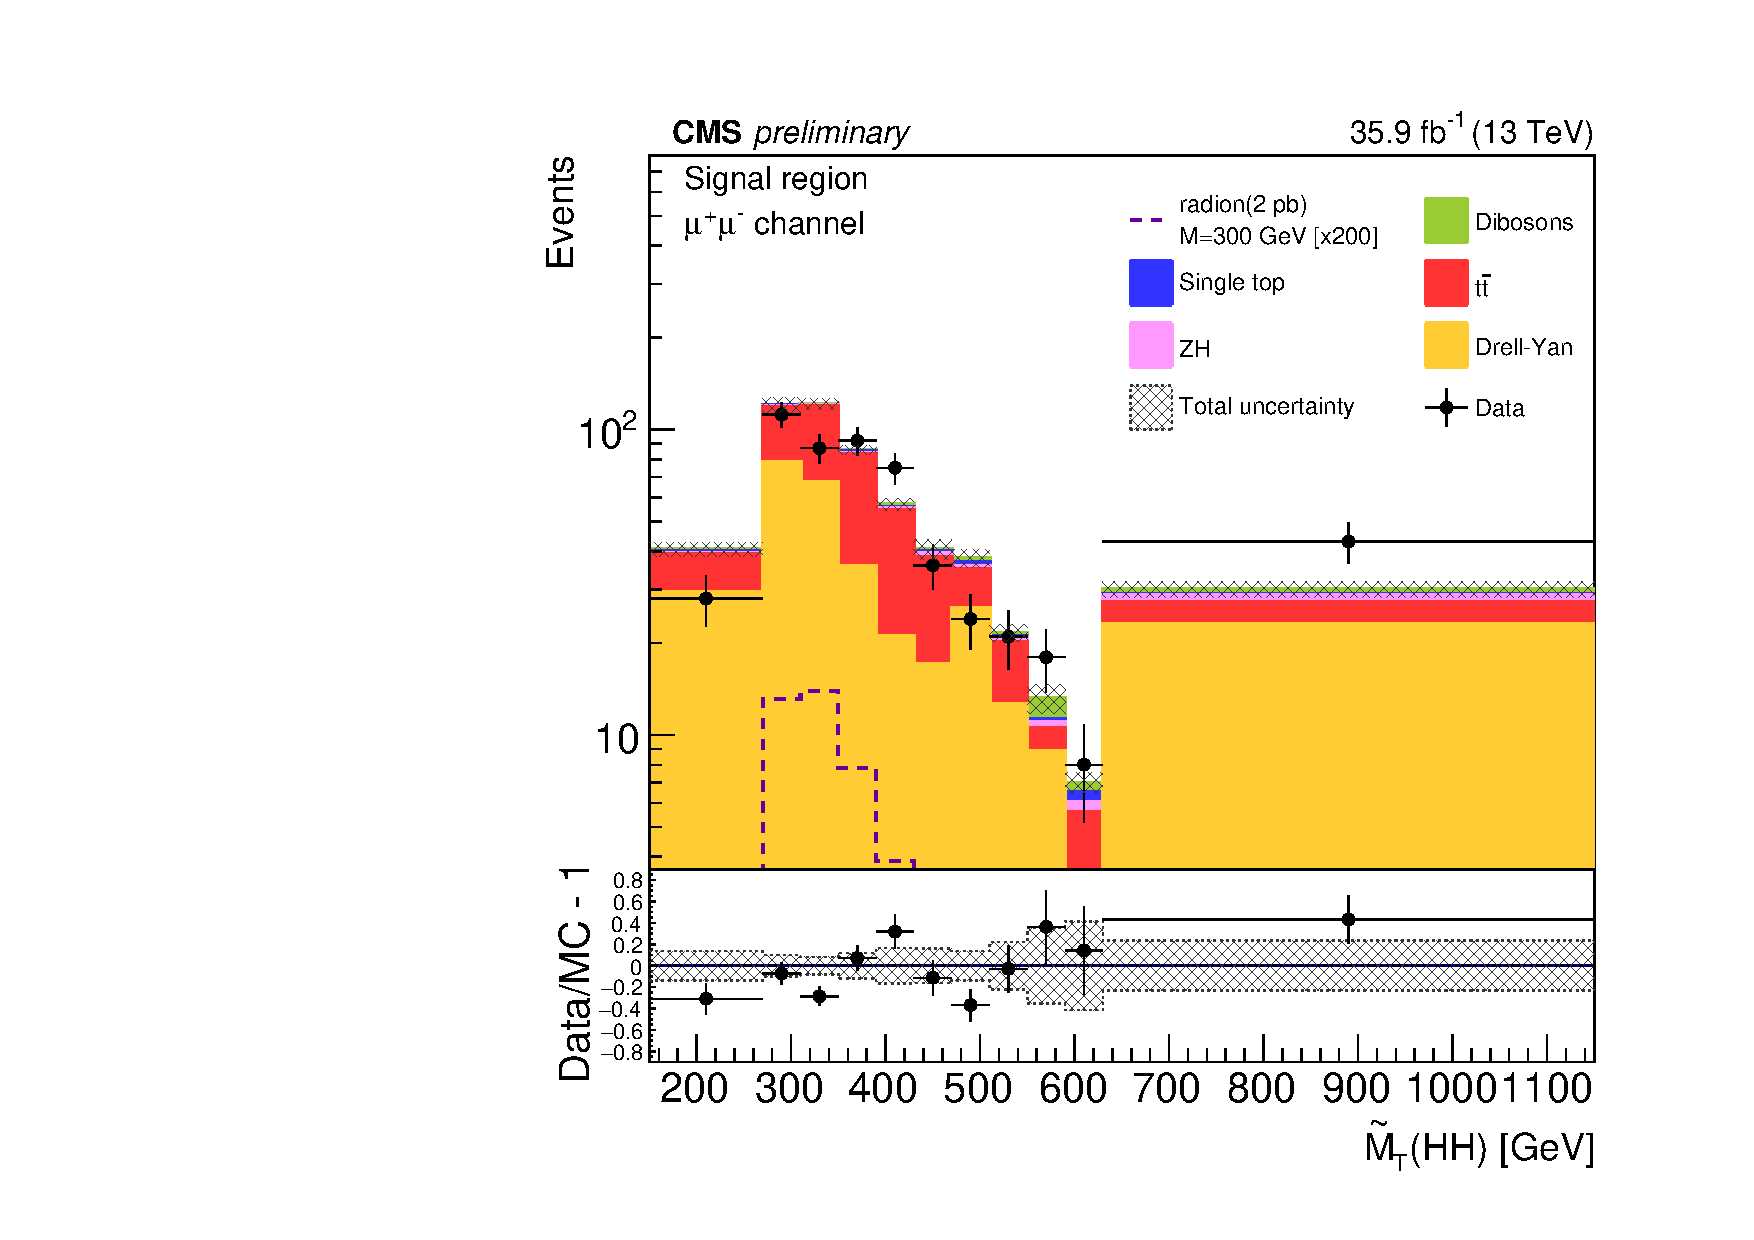
\includegraphics[width=0.31\textwidth]{hhMt_mm_SR_FullPostfit_plot_nov16_2_radion.pdf} \\
    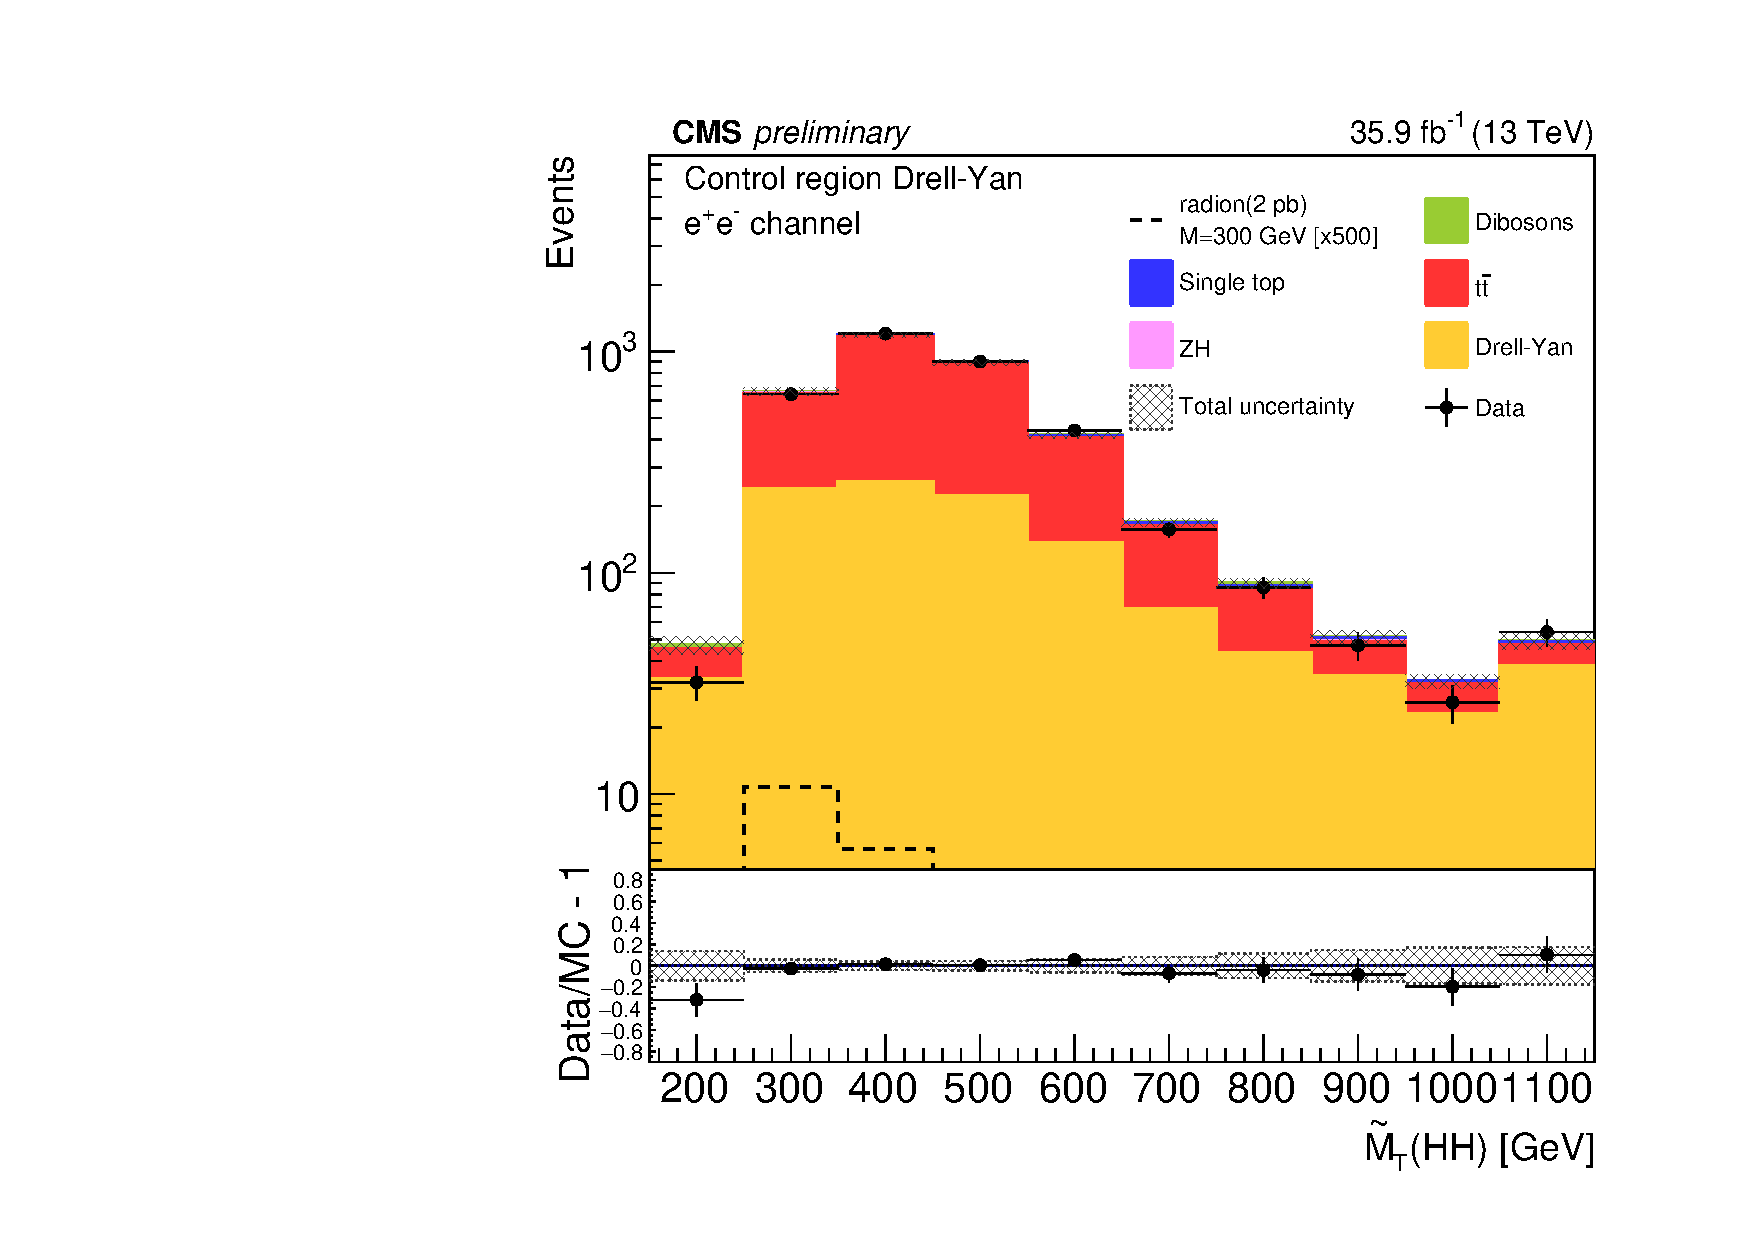
\includegraphics[width=0.31\textwidth]{hhMt_ee_CRDY_FullPostfit_plot_nov16_2_radion.pdf}
    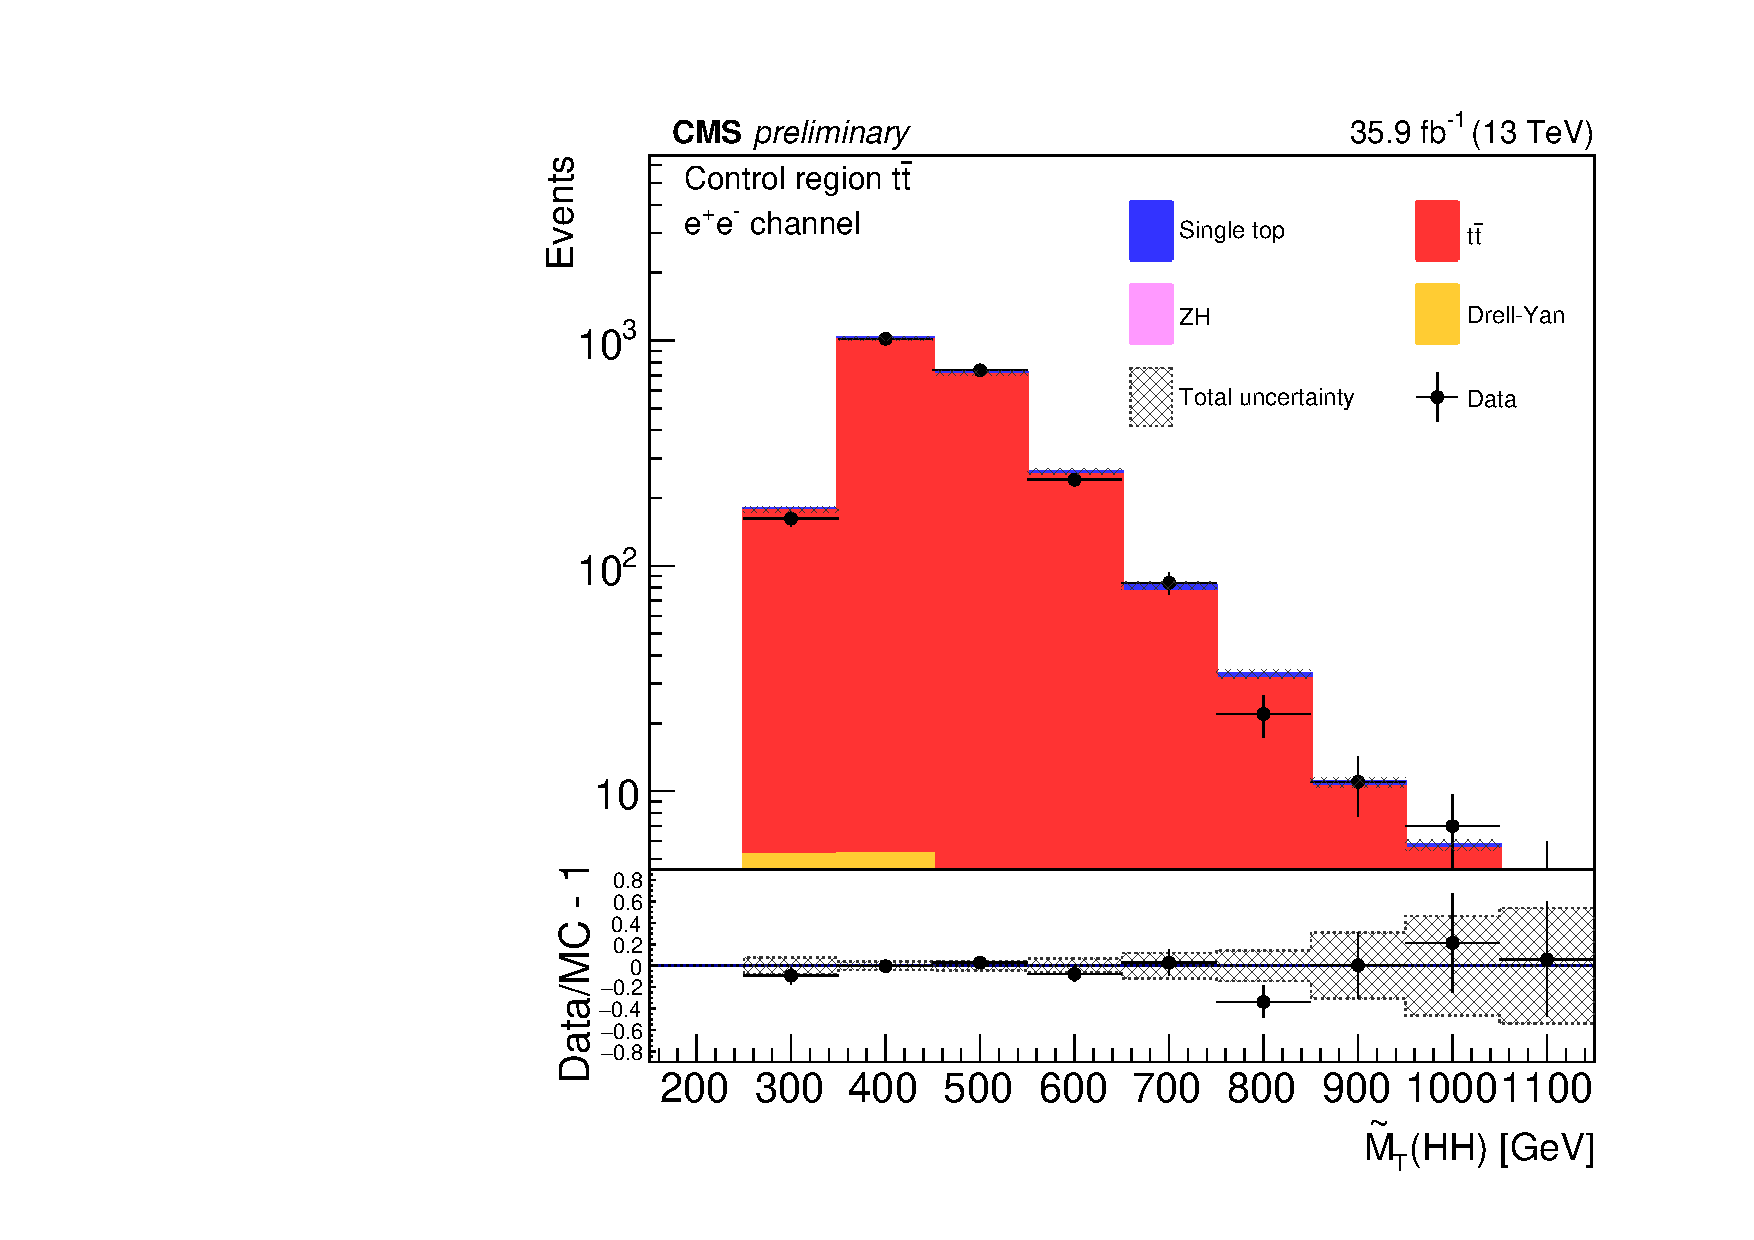
\includegraphics[width=0.31\textwidth]{hhMt_ee_CRTT_FullPostfit_plot_nov16_2_radion.pdf}
    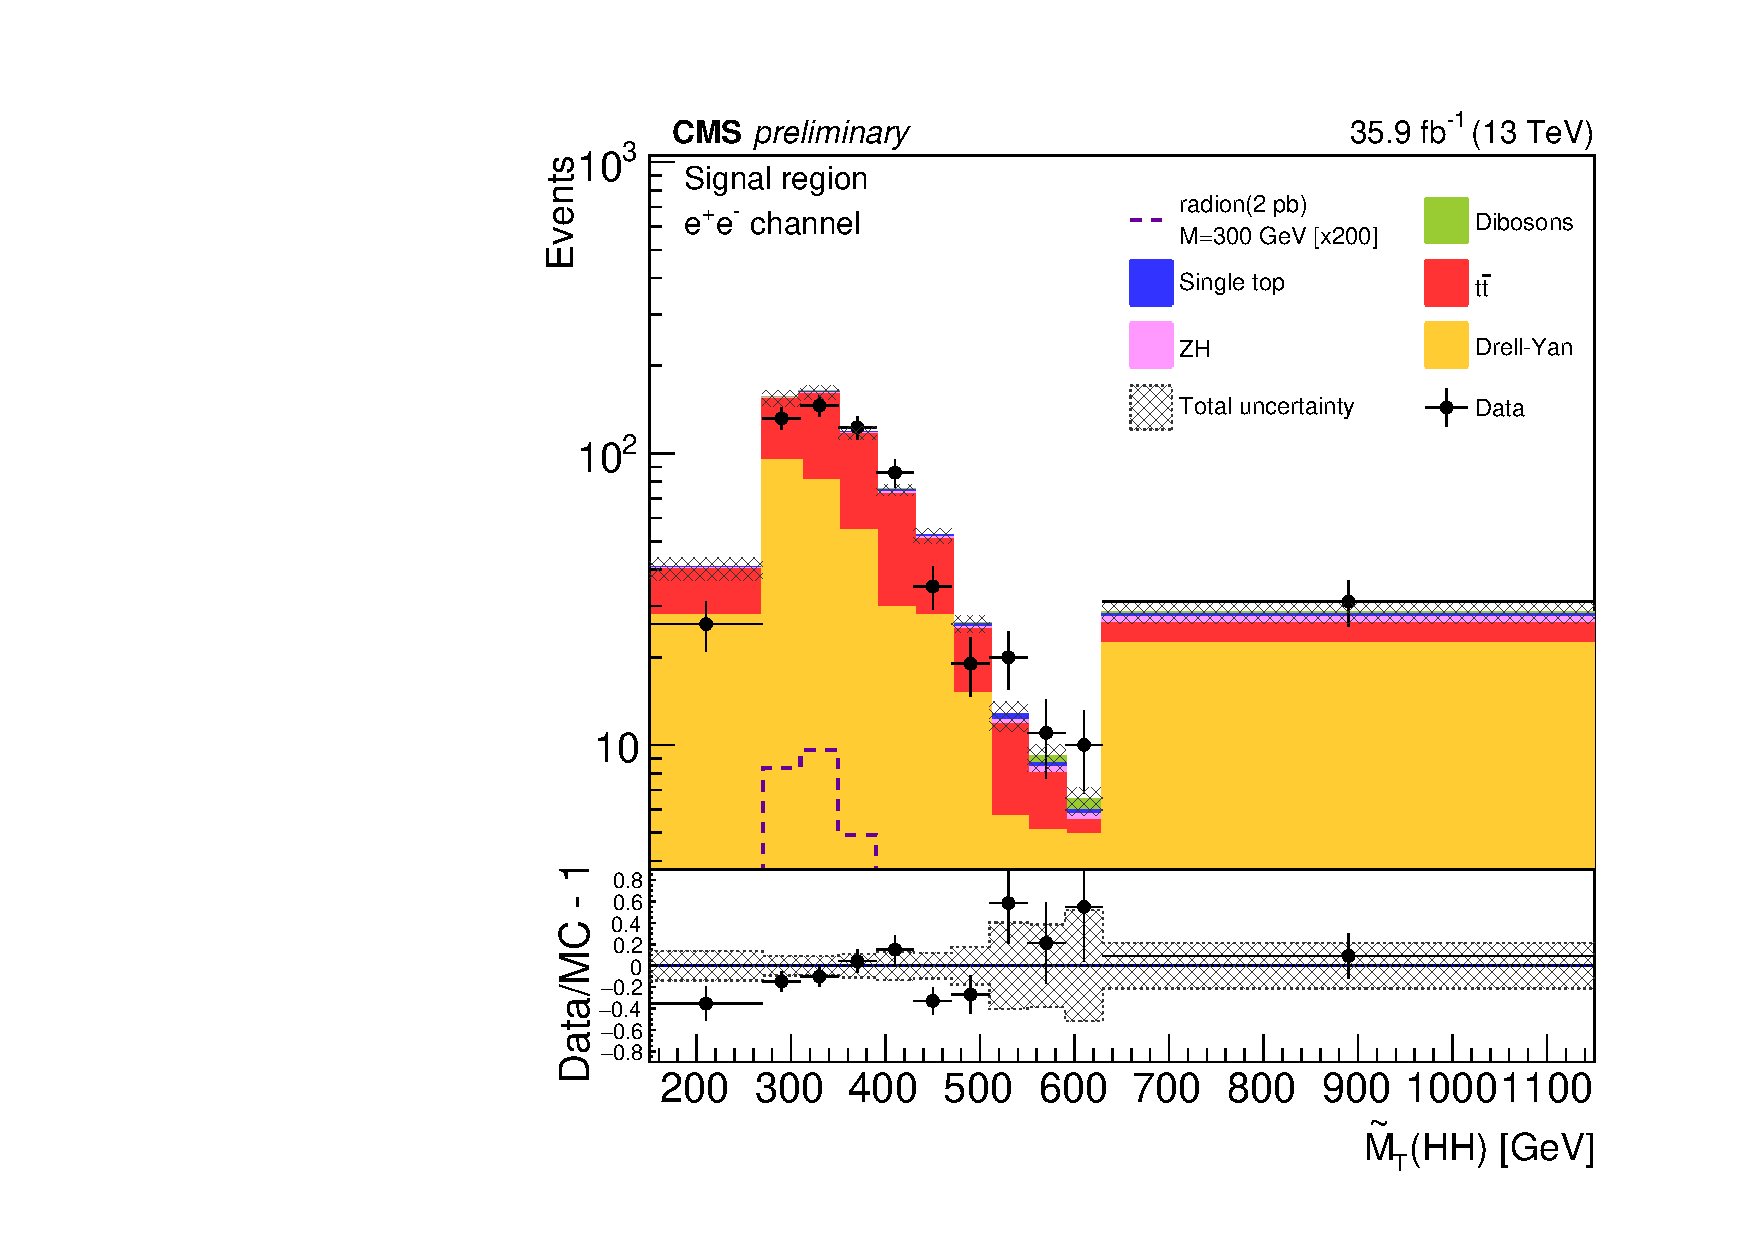
\includegraphics[width=0.31\textwidth]{hhMt_ee_SR_FullPostfit_plot_nov16_2_radion.pdf}
    \caption{Transverse mass of the reconstructed HH candidates for data, the simulated signal radion sample
    for the 300 GeV mass hypothesis, and simulated backgrounds scaled according to the fit results. The top
    row shows the figures for the muon channel while the bottom row is for the electron channel. For each row,
    the left plot is for the Drell-Yan control region, the middle is for the \ttbar control region, and the right
    is for the signal region. Signal normalization choice is discussed in the text. The crosshatched area represents
    the sum of statistical and systematic uncertainties.}
    \label{fig:MCcomparisons_radion}
%                                                                                                                 
% Comparison of data and simulation.  Transverse mass of                                                          
%      the reconstructed HH candidate for 300 GeV signal mass                                                     
%      hypothesis, electron channel. Left: Drell-Yan control region. Middle: \ttbar                               
%      control region. Right: signal region. }                                                                    
%    \label{MCcomparisons_electrons}                                                                              
  \end{center}
\end{figure}







\subsection{Scale Factors}
%\section{HLT Lepton Scale Factors}

Electron ID and ISO scale factors, as well as HLT scale factors (Fig.~\ref{fig:trigger_eff_diele}), have been computed by VHbb group, which ntuples and analysis setup we reutilise. Scale factors have been presented at the EGamma physics object groups (POG) meeting~\cite{egSF} and fully approved. We reuse those scale factors and apply them to our MC samples. 

Muon ID scale factors, as well as ISO scale factors, have been derived separately for runs G/H and B/C/D/E/F runs (2016 data at LHC has been split into several "runs") and then luminosity averaged to obtain the final numbers ~\cite{muonIDnISO}. Tracker scale factors (~\ref{fig:trigger_eff_diele}) are taken from the Muon POG twiki page~\cite{muonTRK} and used as is. HLT dimuon scale factors were derived by VHbb group and further approved by the muon POG. These scale factors were derived separately for run H (Fig.~\ref{fig:trigger_SF_dimu_H}) and B/C/D/E/F/G (Fig.~\ref{fig:trigger_SF_dimu_BCDEFG}) runs and then luminosity averaged ~\cite{muonTrigger}. On top, separate scale factors are calculated for the dZ requirement of HLT\_Mu17\_TrkIsoVVL\_Mu8\_TrkIsoVV\L\_DZ\_v* OR HLT\_Mu17\_TrkIsoVVL\_TkMu8\_TrkIsoVVL\_DZ\_v* triggers, using dilepton events that have already passed the HLT\_Mu17\_TrkIsoVVL\_Mu8\_TrkIsoVVL\_v* OR HLT\_Mu17\_TrkIsoVVL\_TkMu8\_TrkIsoVVL\_v* triggers (Fig. ~\ref{fig:trigger_SF_dimu_dZ_H}).



\section{BDT Discriminant}
\label{sec:BDT}

The Toolkit for Multivariate Data Analysis with ROOT (TMVA) package is used to perform BDT training~\cite{Hocker:2007ht}. This ROOT-integrated library enables the usage of the machine learning techniques for the physics data analysis and is commonly used. 

\subsection{Construction of the BDT}
In this analysis we use the set of nine variables to construct the BDT. These variables are the same in both low and high mass trainings and for both heavy resonances.

Some variables are important only in the specific mass regime, some are ranked highly universally across the whole mass range. For example, in the low mass regime \ETmiss and \HBB~ mass are powerful discriminators against Drell-Yan to leptons plus jets. That is why these
observables are located in the top three variables of the ranking for low mass BDT (Figs. ~\ref{fig:ranking}). In the high mass regime the leverage is in the boost, therefore, $\Delta R = \sqrt{\Delta \phi^2 + \Delta \eta^2}$ variables, as well as $p_{T}$-related variables show high performance (Figs. ~\ref{fig:ranking}). Namely, $p_{T}$ of both Higgs bosons, Z boson, and also
separation $\Delta R $  between two b-jets and also $\Delta R$ between  two leptons. It is worth noting that \HBB~ mass is a powerful discriminator ranked highly for all mass regimes and both channels. Plots of input variables and correlations are shown on the Figs. ~\ref{fig:ele_lowVars}, ~\ref{fig:muon_lowVars}, ~\ref{fig:ele_cors_low}, ~\ref{fig:ele_cors_high}, ~\ref{fig:muon_cors_low}, ~\ref{fig:muon_cors_high}.

\begin{figure}[tbp]
  \begin{center}
   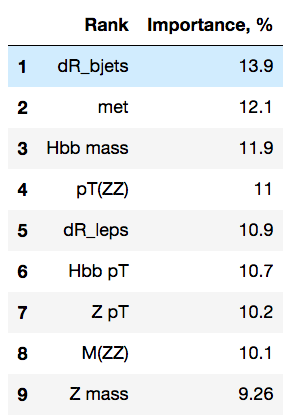
\includegraphics[width=0.35\textwidth]{ee_low.png}
   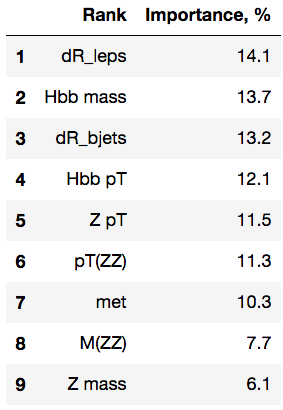
\includegraphics[width=0.35\textwidth]{ee_high.png}\\
   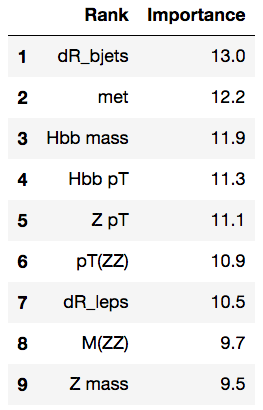
\includegraphics[width=0.35\textwidth]{mm_low.png}
   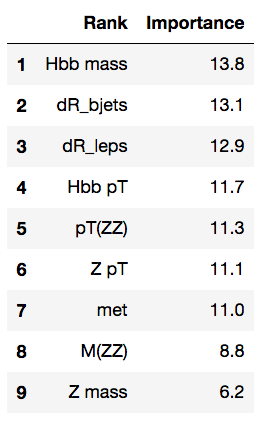
\includegraphics[width=0.35\textwidth]{mm_high.png}
    \caption{ Ranking of variables in the BDT training for electron(muon) channel at the top(bottom). Left: low mass BDT. Right: high mass BDT.}
    \label{fig:ranking}
  \end{center}
\end{figure}


\begin{figure}[tbp]
  \begin{center}
   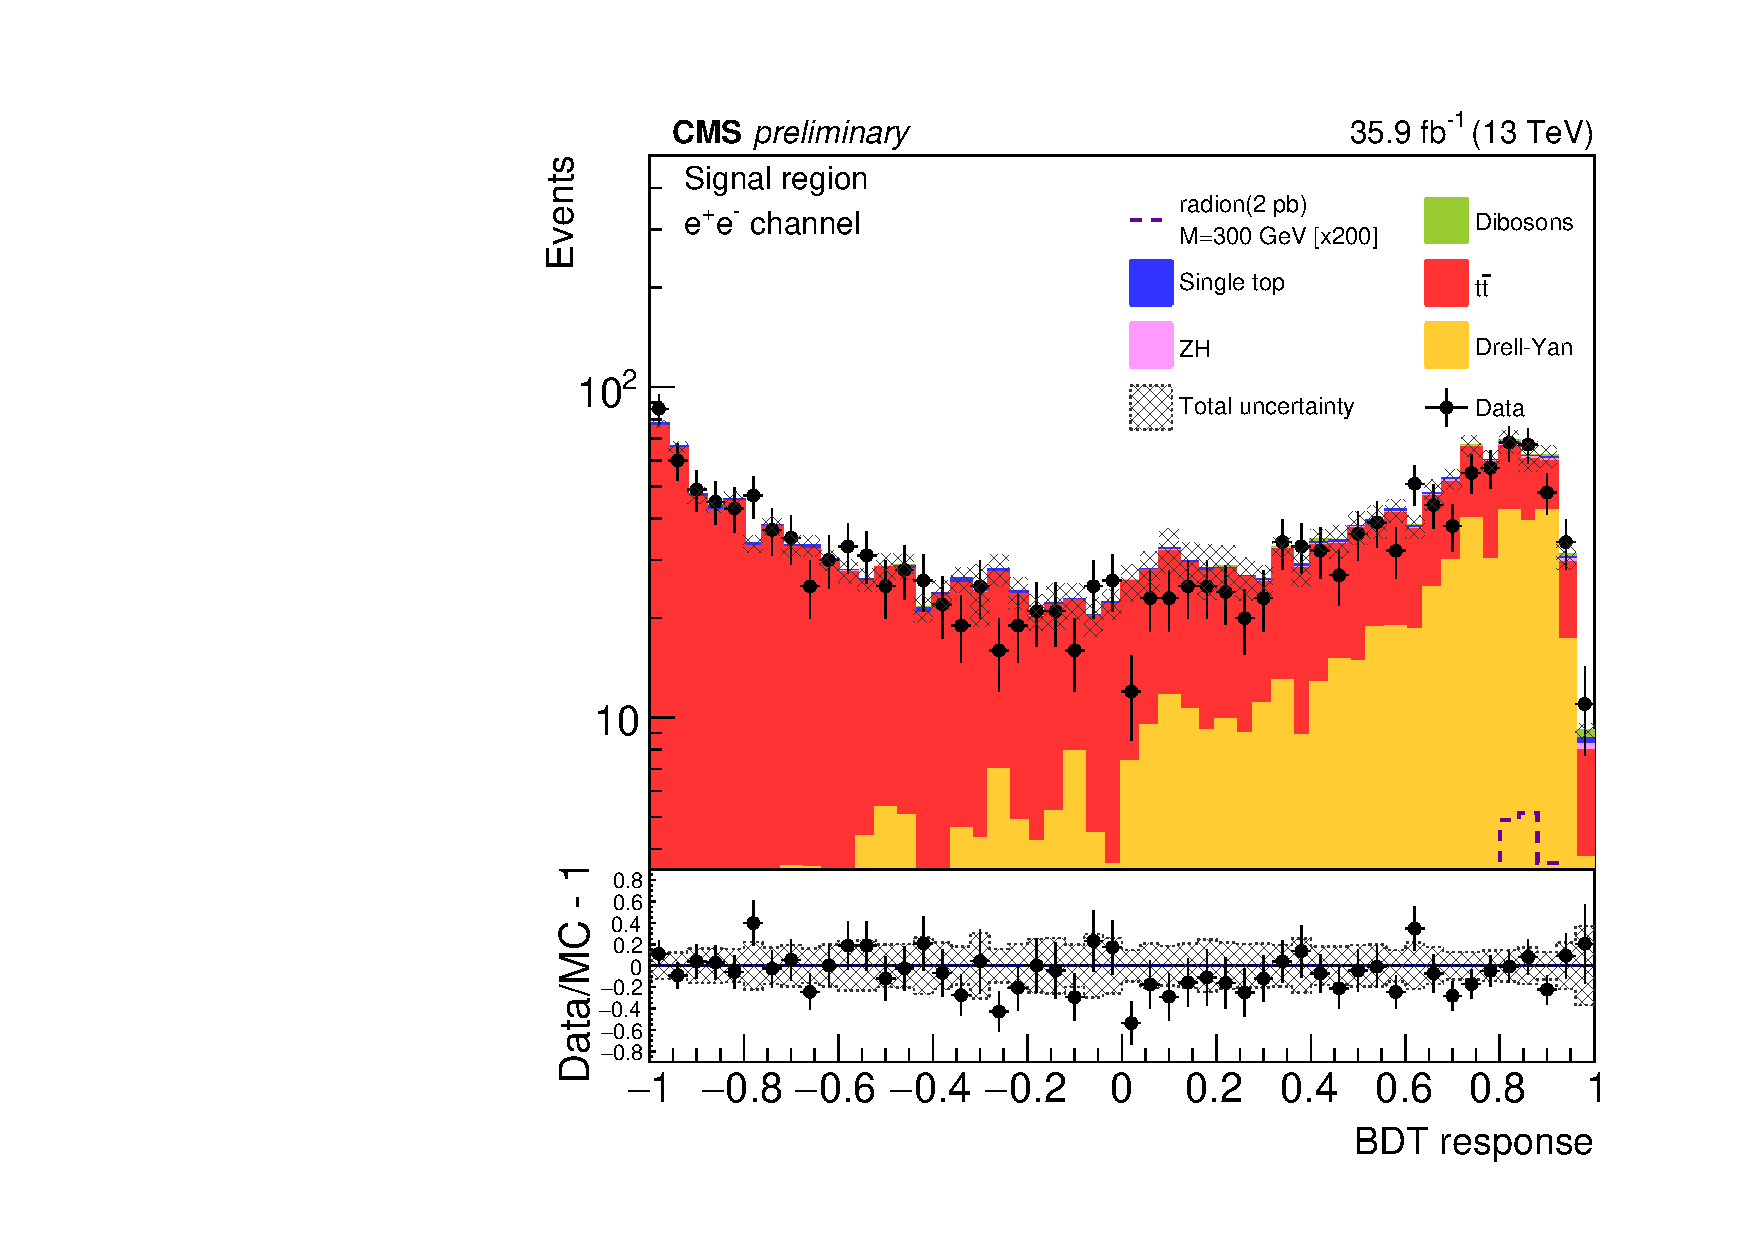
\includegraphics[width=0.6\textwidth]{bdt_response_ee_SR_FullPostfit_plot_nov16_2_radion.pdf}\\
   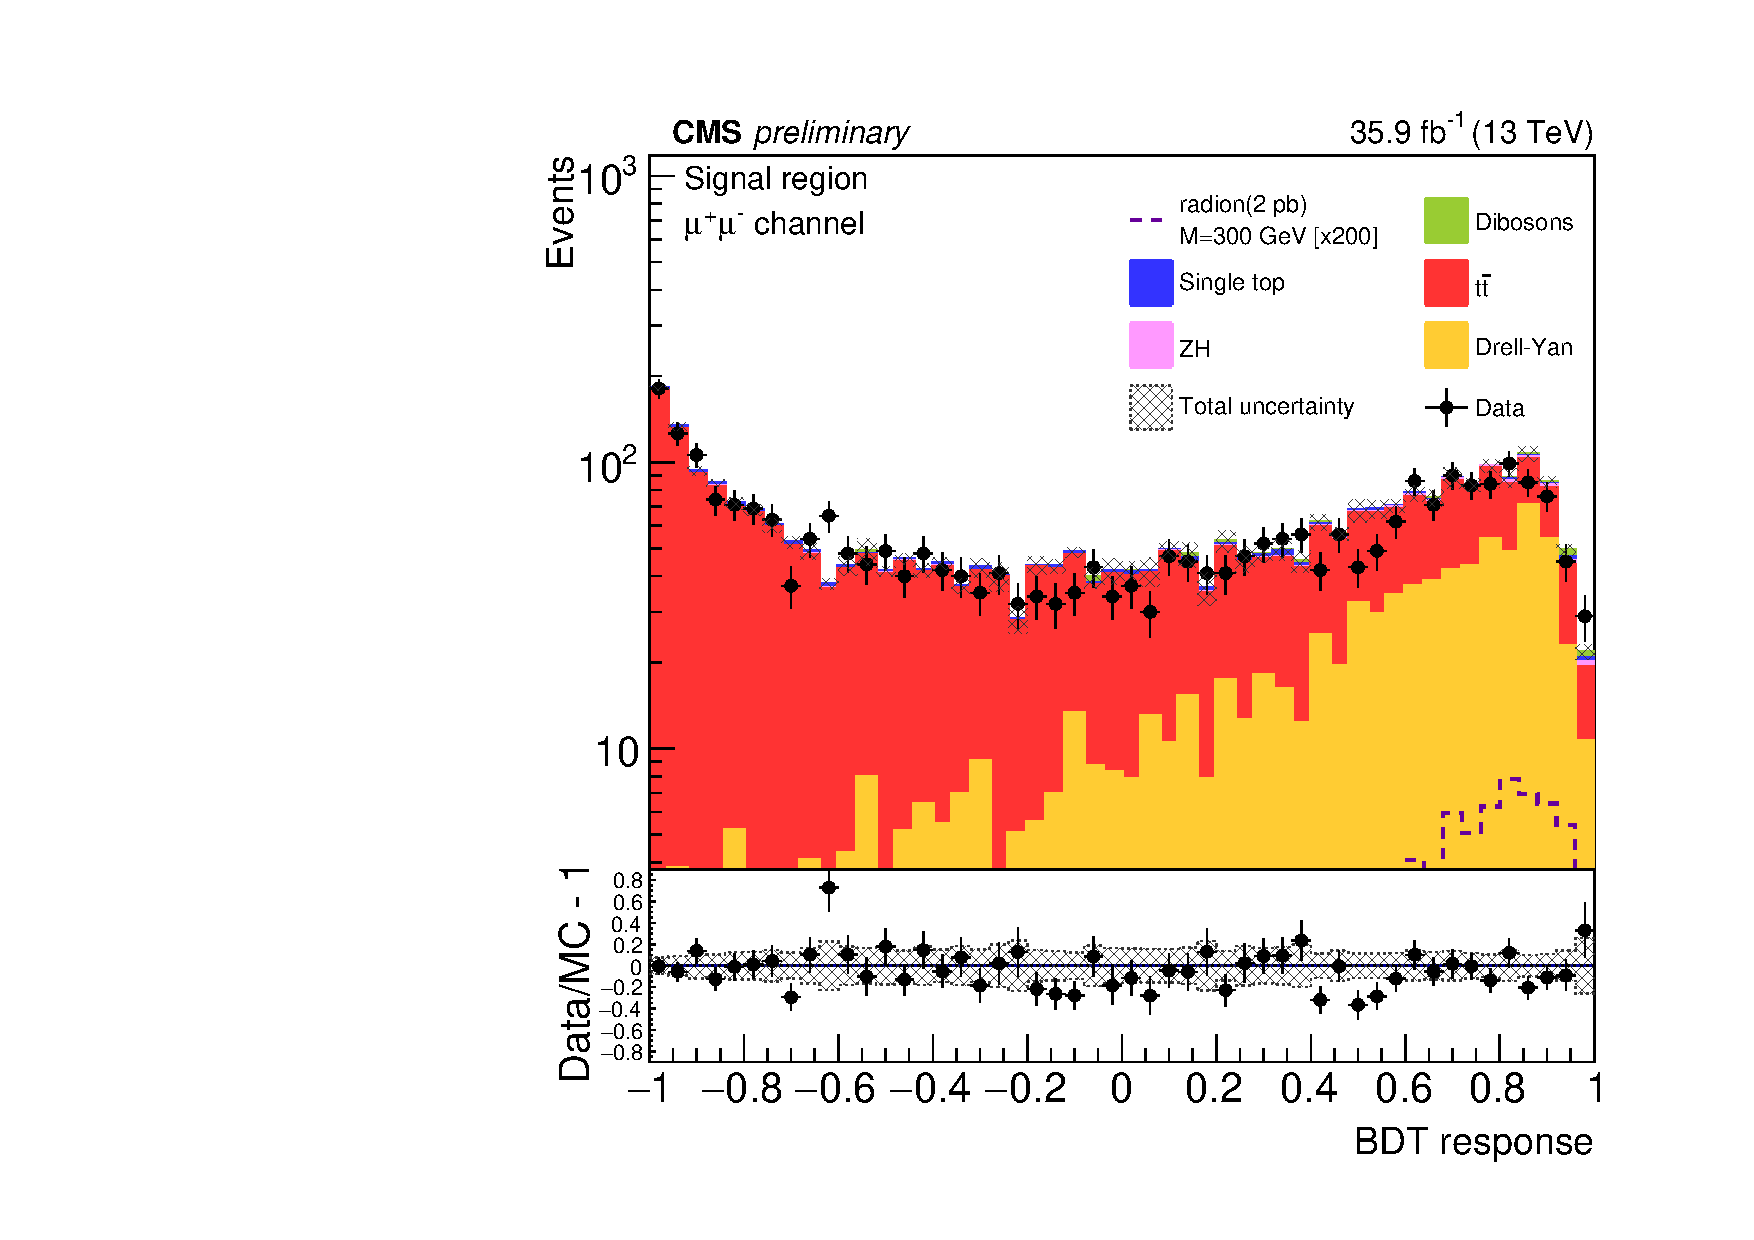
\includegraphics[width=0.6\textwidth]{bdt_response_mm_SR_FullPostfit_plot_nov16_2_radion.pdf}\\
    \caption{ BDT plots for radion case, electron(muon) channel at the top(bottom). Signal region, 300 GeV mass hypothesis. For electrons cut is at 0.4, for muons at 0.7. More details at the table \ref{suboptCut}.}
    \label{fig:BDTs}
  \end{center}
\end{figure}




\begin{figure}[tbp]
  \begin{center}
   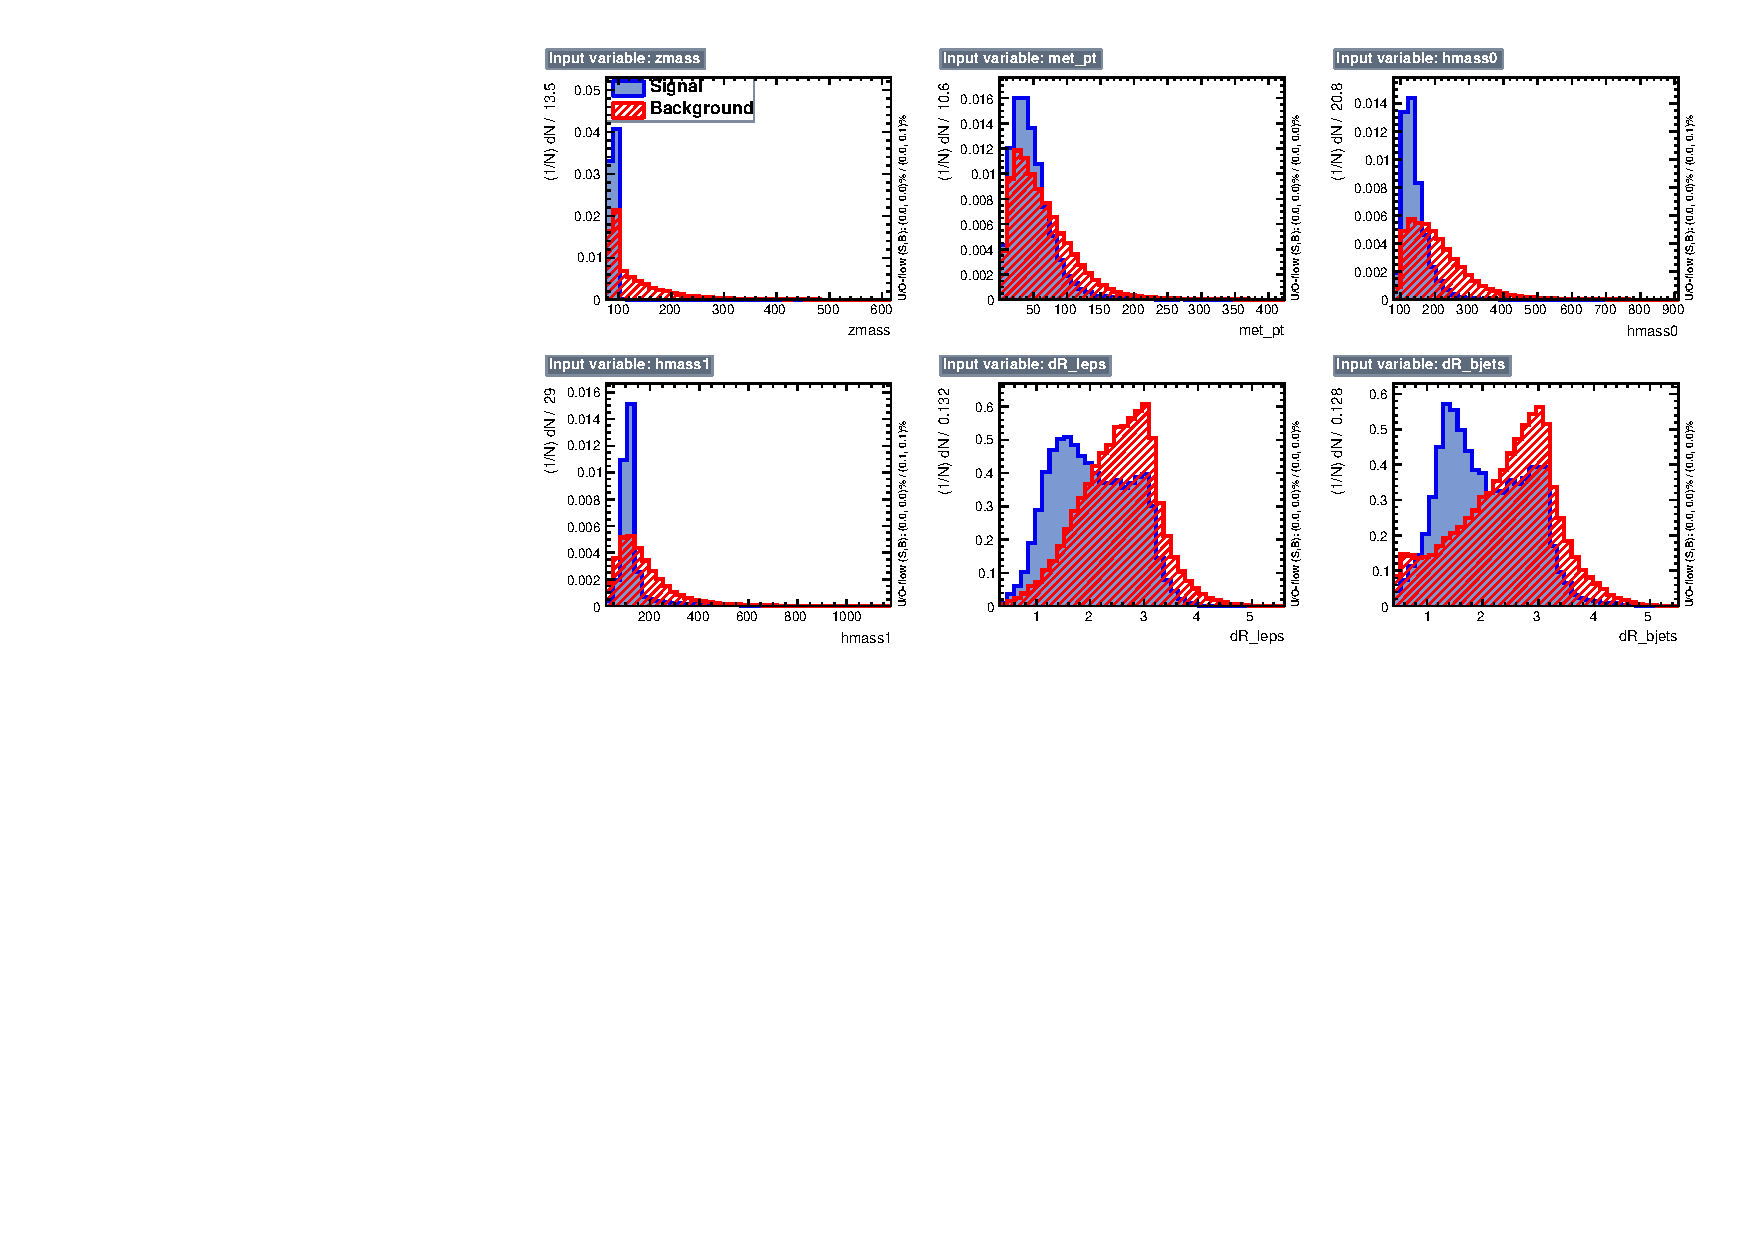
\includegraphics[width=0.95\textwidth]{bdtPlots_eles/low_vars1.pdf}
   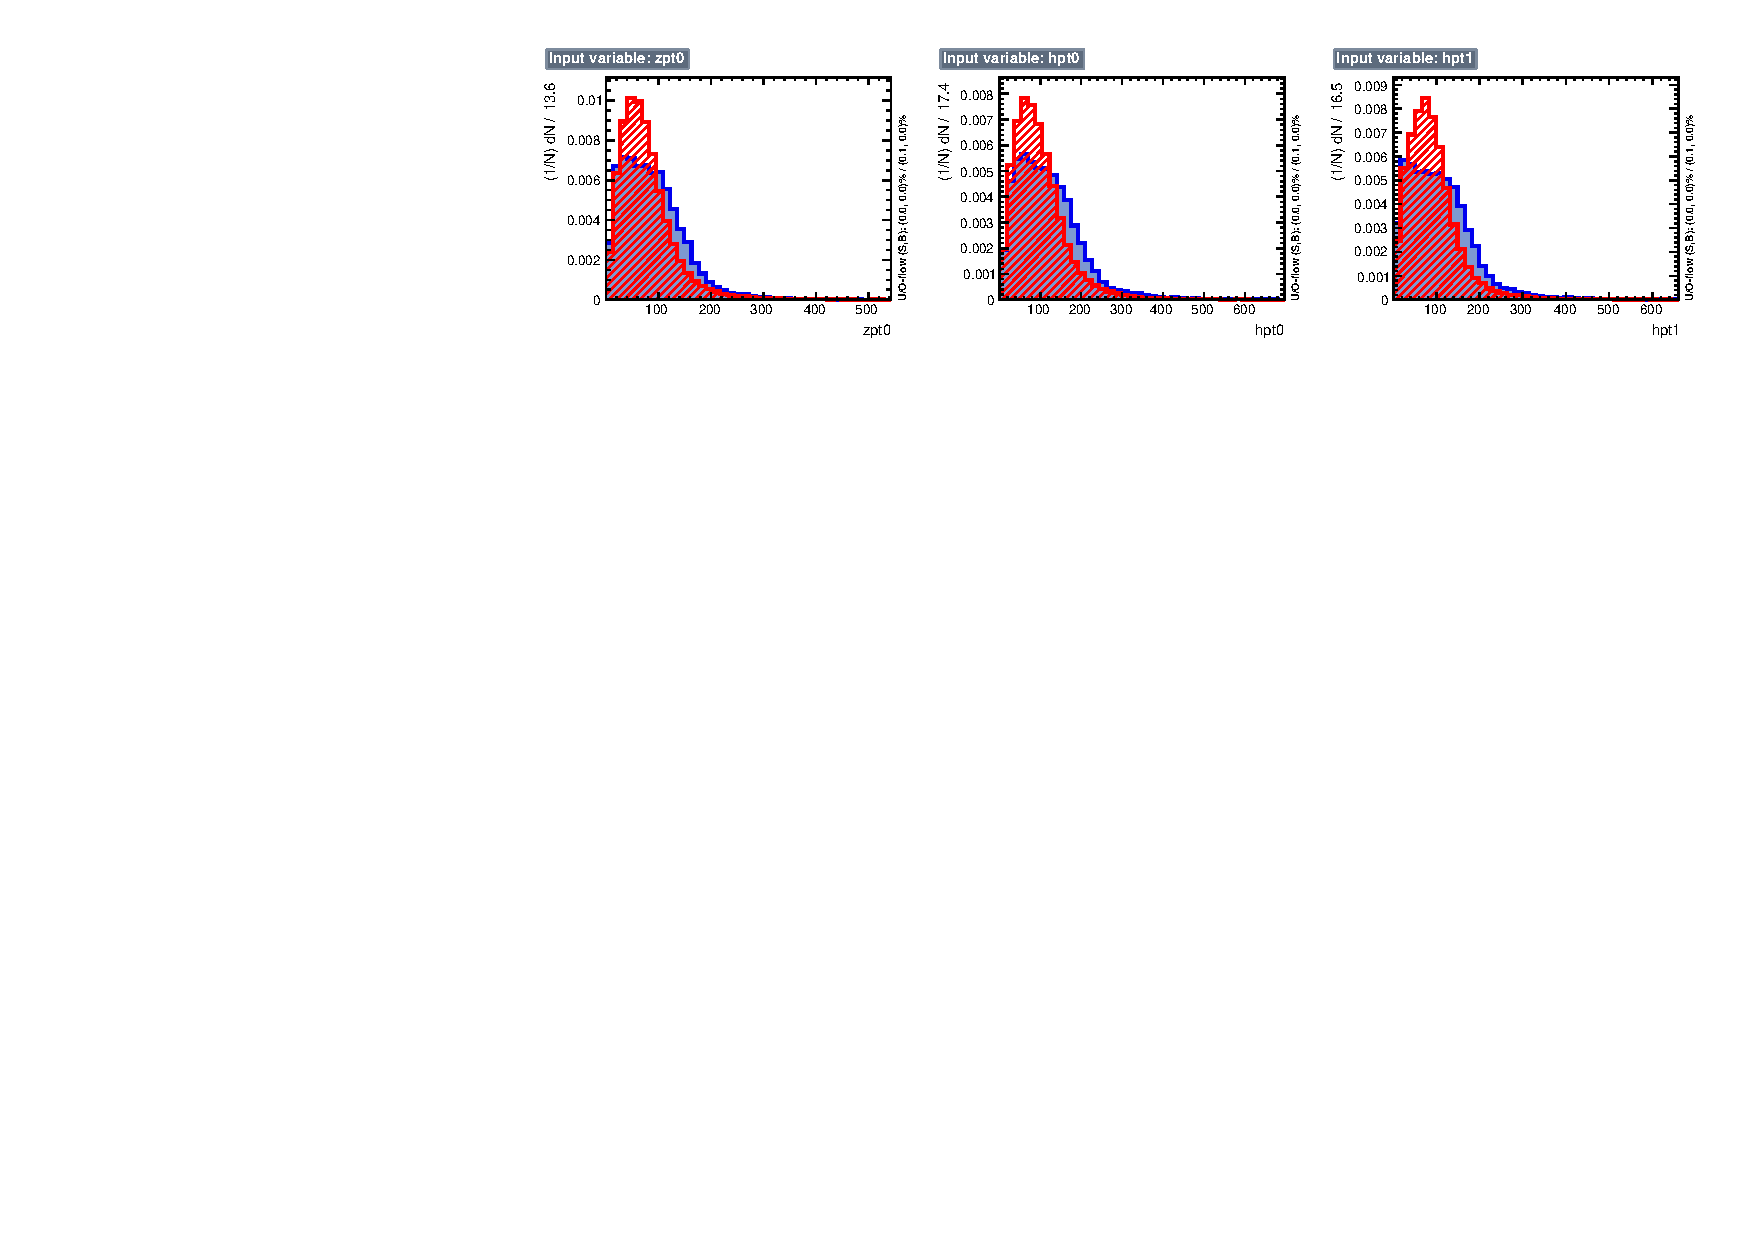
\includegraphics[width=0.95\textwidth]{bdtPlots_eles/low_vars2.pdf}
    \caption{ Variables used in the low mass training for electron channel. Index '1' refers to \bbbar and index '0' refers to ZZ.}
    \label{fig:ele_lowVars}
  \end{center}
\end{figure}



\begin{figure}[tbp]
  \begin{center}
   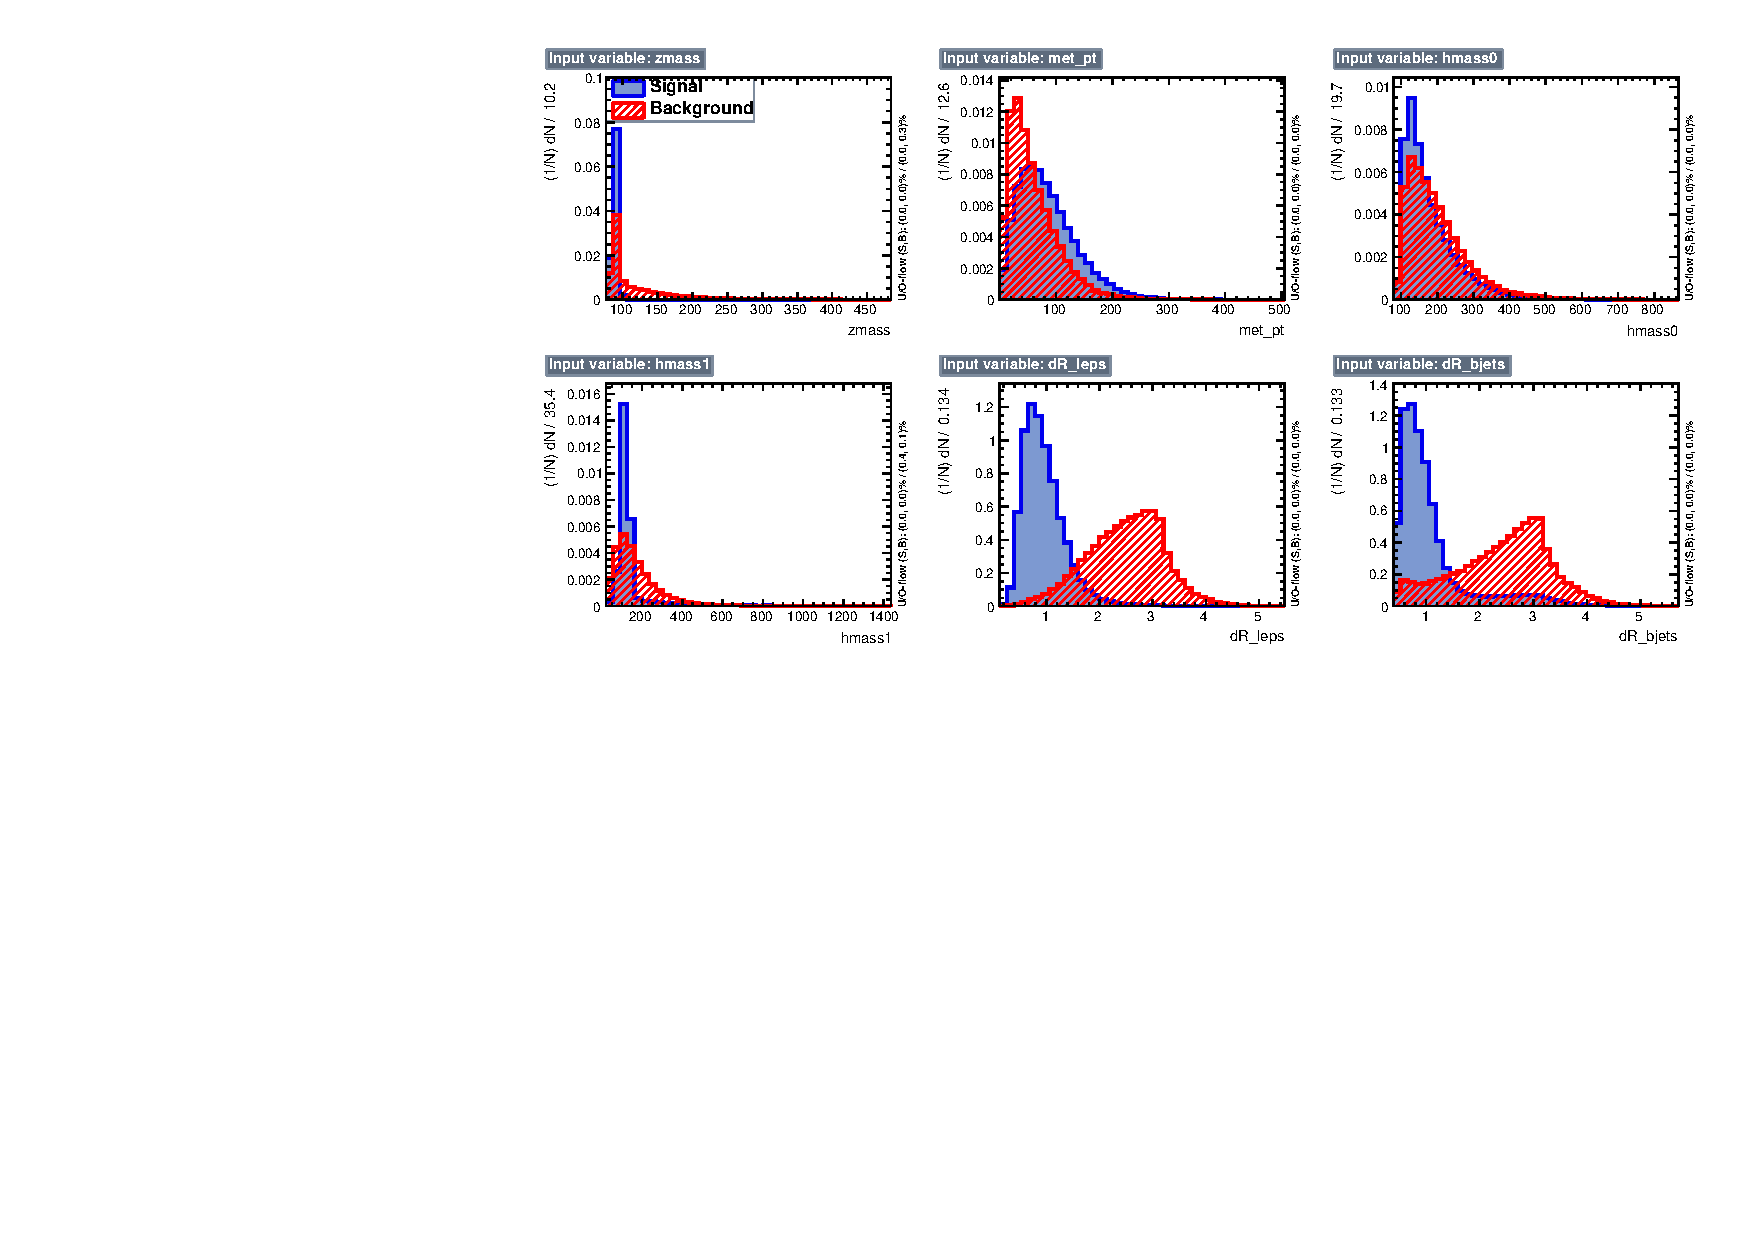
\includegraphics[width=0.95\textwidth]{bdtPlots_eles/high_vars1.pdf}
   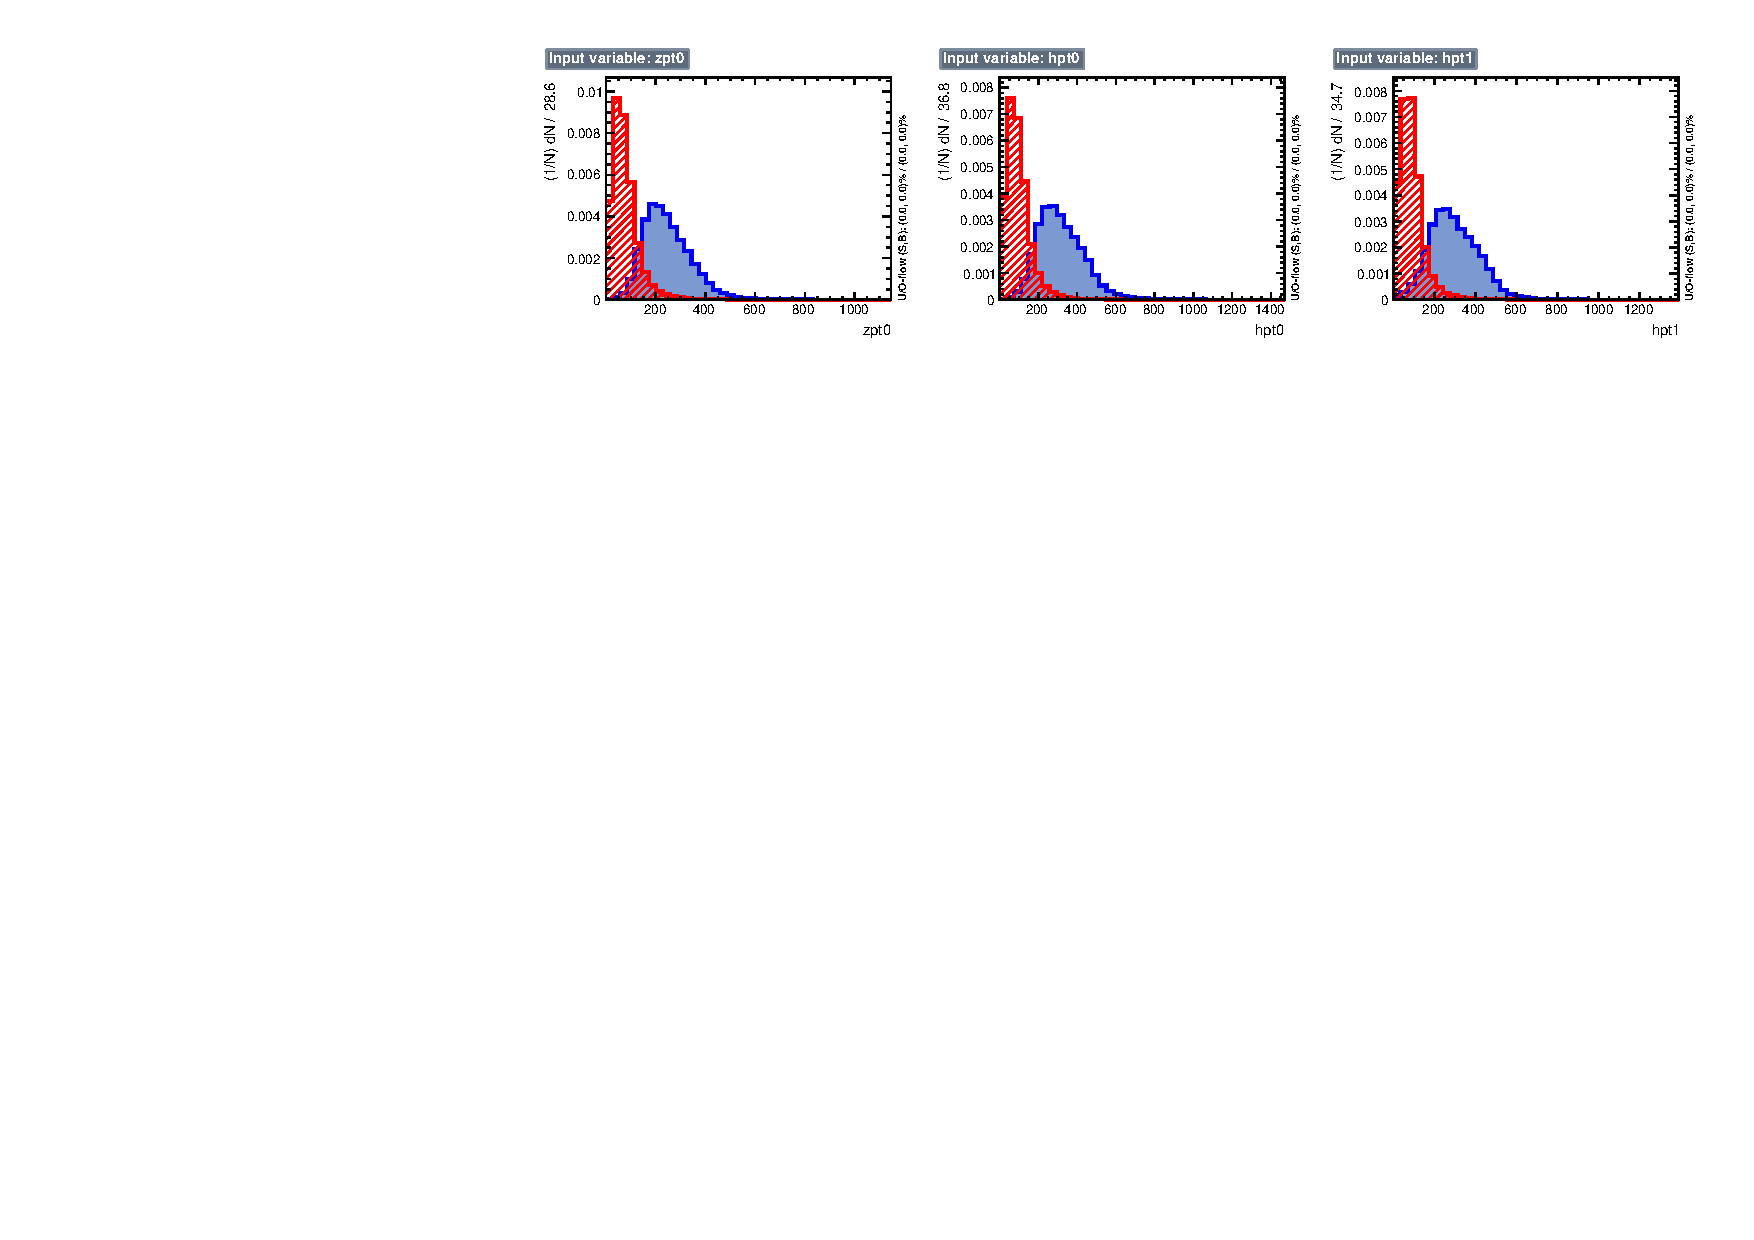
\includegraphics[width=0.95\textwidth]{bdtPlots_eles/high_vars2.pdf}
    \caption{ Variables used in the high mass training for electron channel.}
    \label{fig:ele_highVars}
  \end{center}
\end{figure}


It is hard to get high performance in the low mass training, since
this is where all the backgrounds are concentrated (Figs. ~\ref{fig:ele_lowVars}, ~\ref{fig:muon_lowVars}). The rate of background in this region is enormous and most variables have similar distributions for signal and backgrounds. However, BDT performance is noticeably better than what can be achieved using a simple linear discriminant method (Figs. ~\ref{fig:ele_BDTs}, ~\ref{fig:ele_ROCs}, ~\ref{fig:muon_BDTs}, ~\ref{fig:muon_ROCs}). 

Earlier versions of the analysis tried more granular approach to the number of BDTs, up to four BDTs to cover the whole range from 250 to 1000 GeV. But it was shown that this added extra complexity brings almost no improvement, while in fact is error prone and computationally twice more expensive. This is why other HH analyses also split the whole mass range only in two subranges and we followed the same suggestion. The BTD plots for radion case in the signal regions for 300 GeV mass hypothesis are shown at Fig. \ref{fig:BDTs}.



\begin{figure}[tbp]
  \begin{center}
   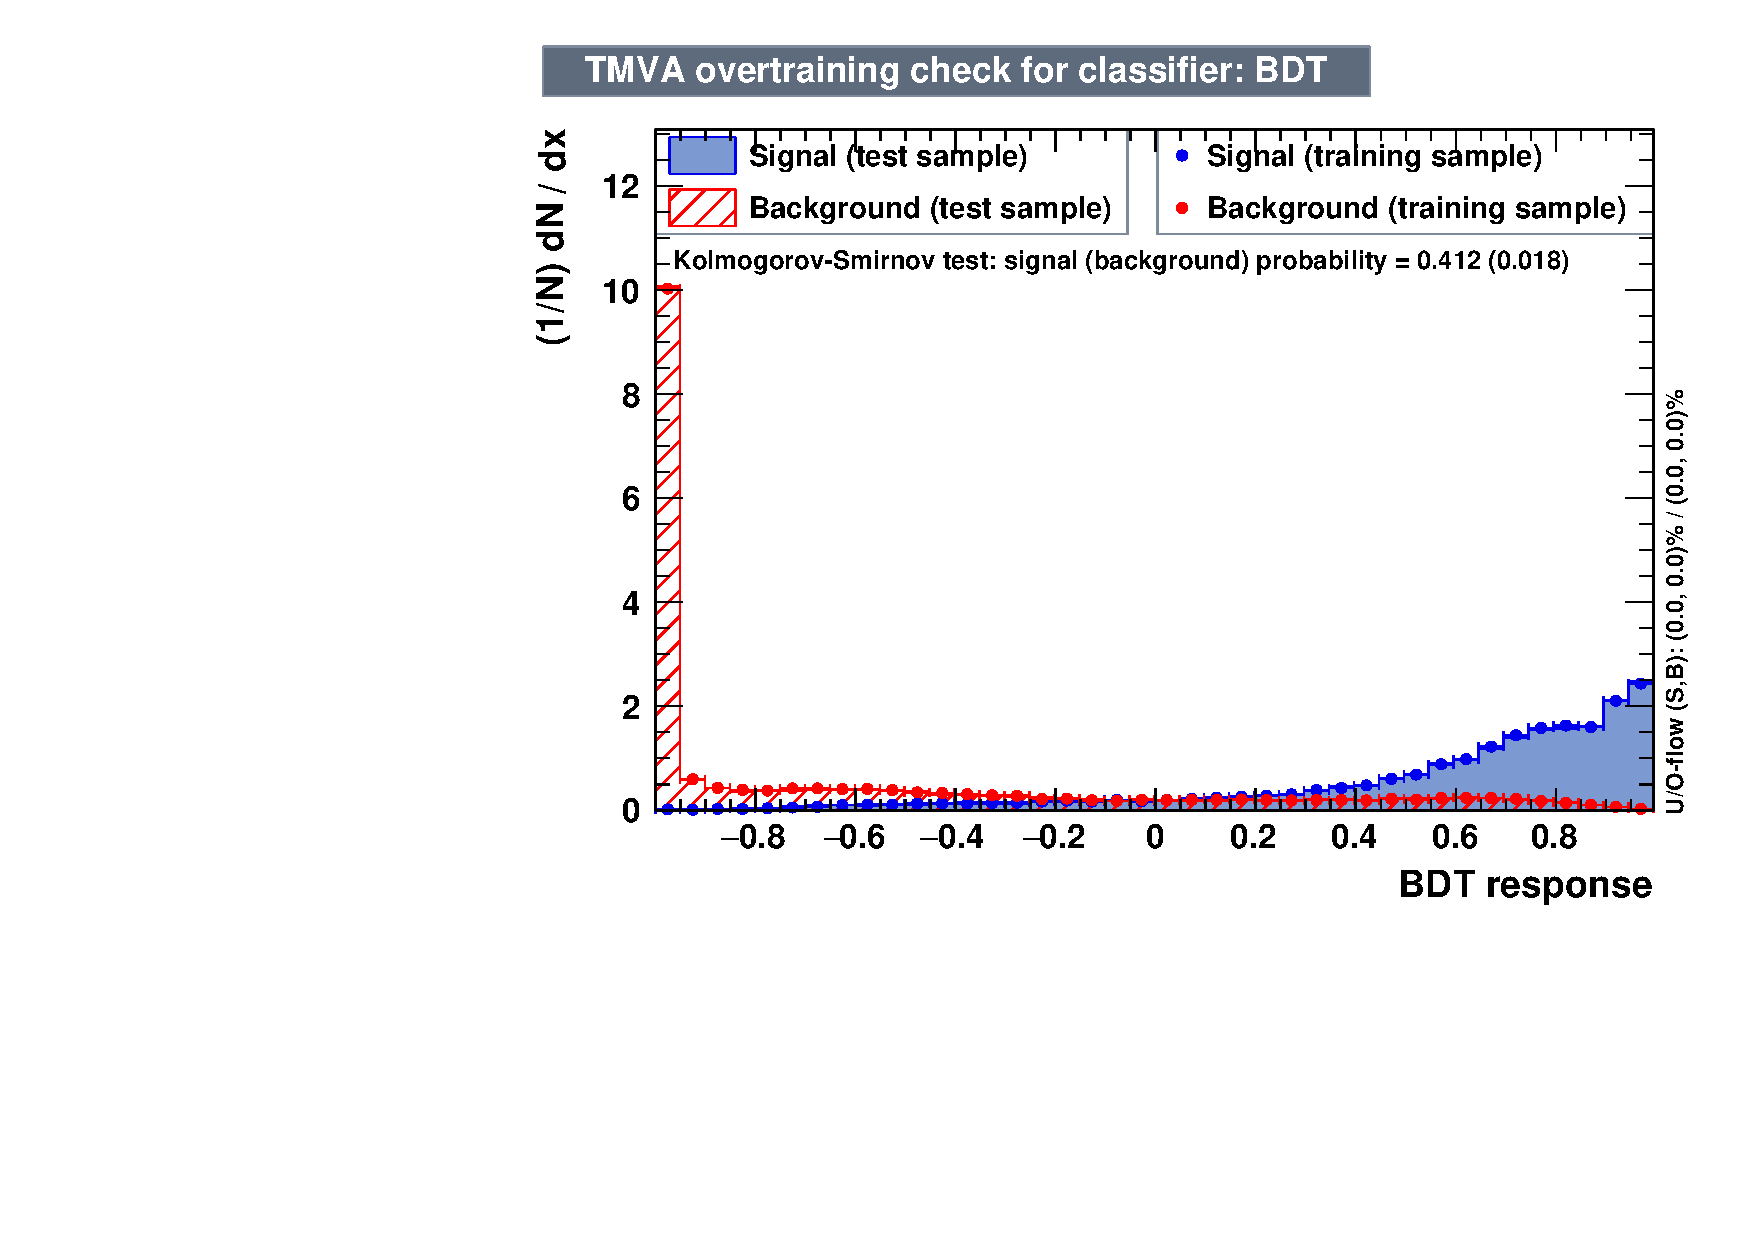
\includegraphics[width=0.75\textwidth]{bdtPlots_eles/low_bdt.pdf}
   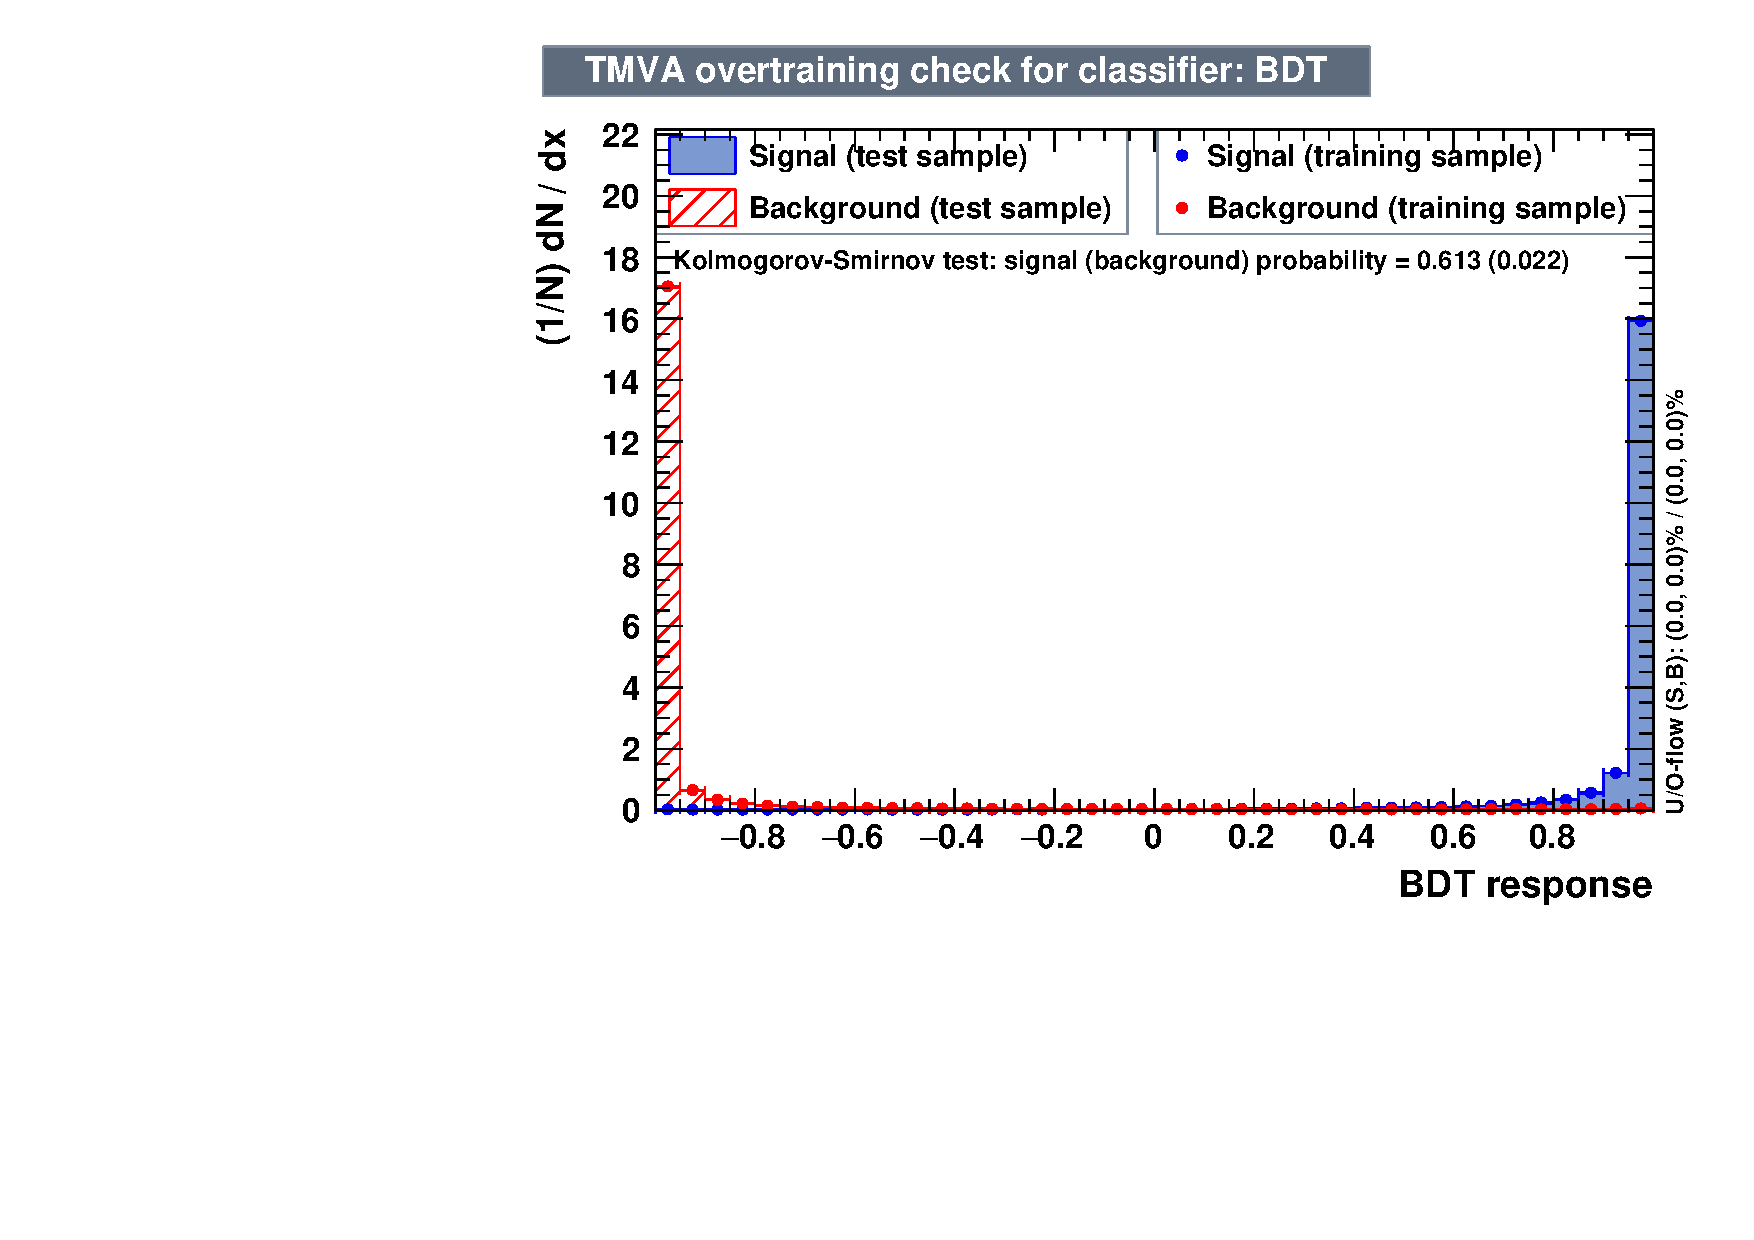
\includegraphics[width=0.75\textwidth]{bdtPlots_eles/high_bdt.pdf}
    \caption{ BDT discriminants for electron channel. Top: low mass training. Bottom: high mass training. }
    \label{fig:ele_BDTs}
  \end{center}
\end{figure}

Performance of the high mass training is perfect (Figs. ~\ref{fig:ele_highVars}, ~\ref{fig:muon_highVars}, ). The ROC curves are close to the top right corner of the efficiencies space, which means a high signal efficiency is achieved along side with the low efficiency of the background. This is due to the
fact that most backgrounds peak in the low mass region. Even linear
discriminant is performing well in this situation (Figs. ~\ref{fig:ele_BDTs}, ~\ref{fig:ele_ROCs}, ~\ref{fig:muon_BDTs}, ~\ref{fig:muon_ROCs}).

\begin{figure}[tbp]
  \begin{center}
   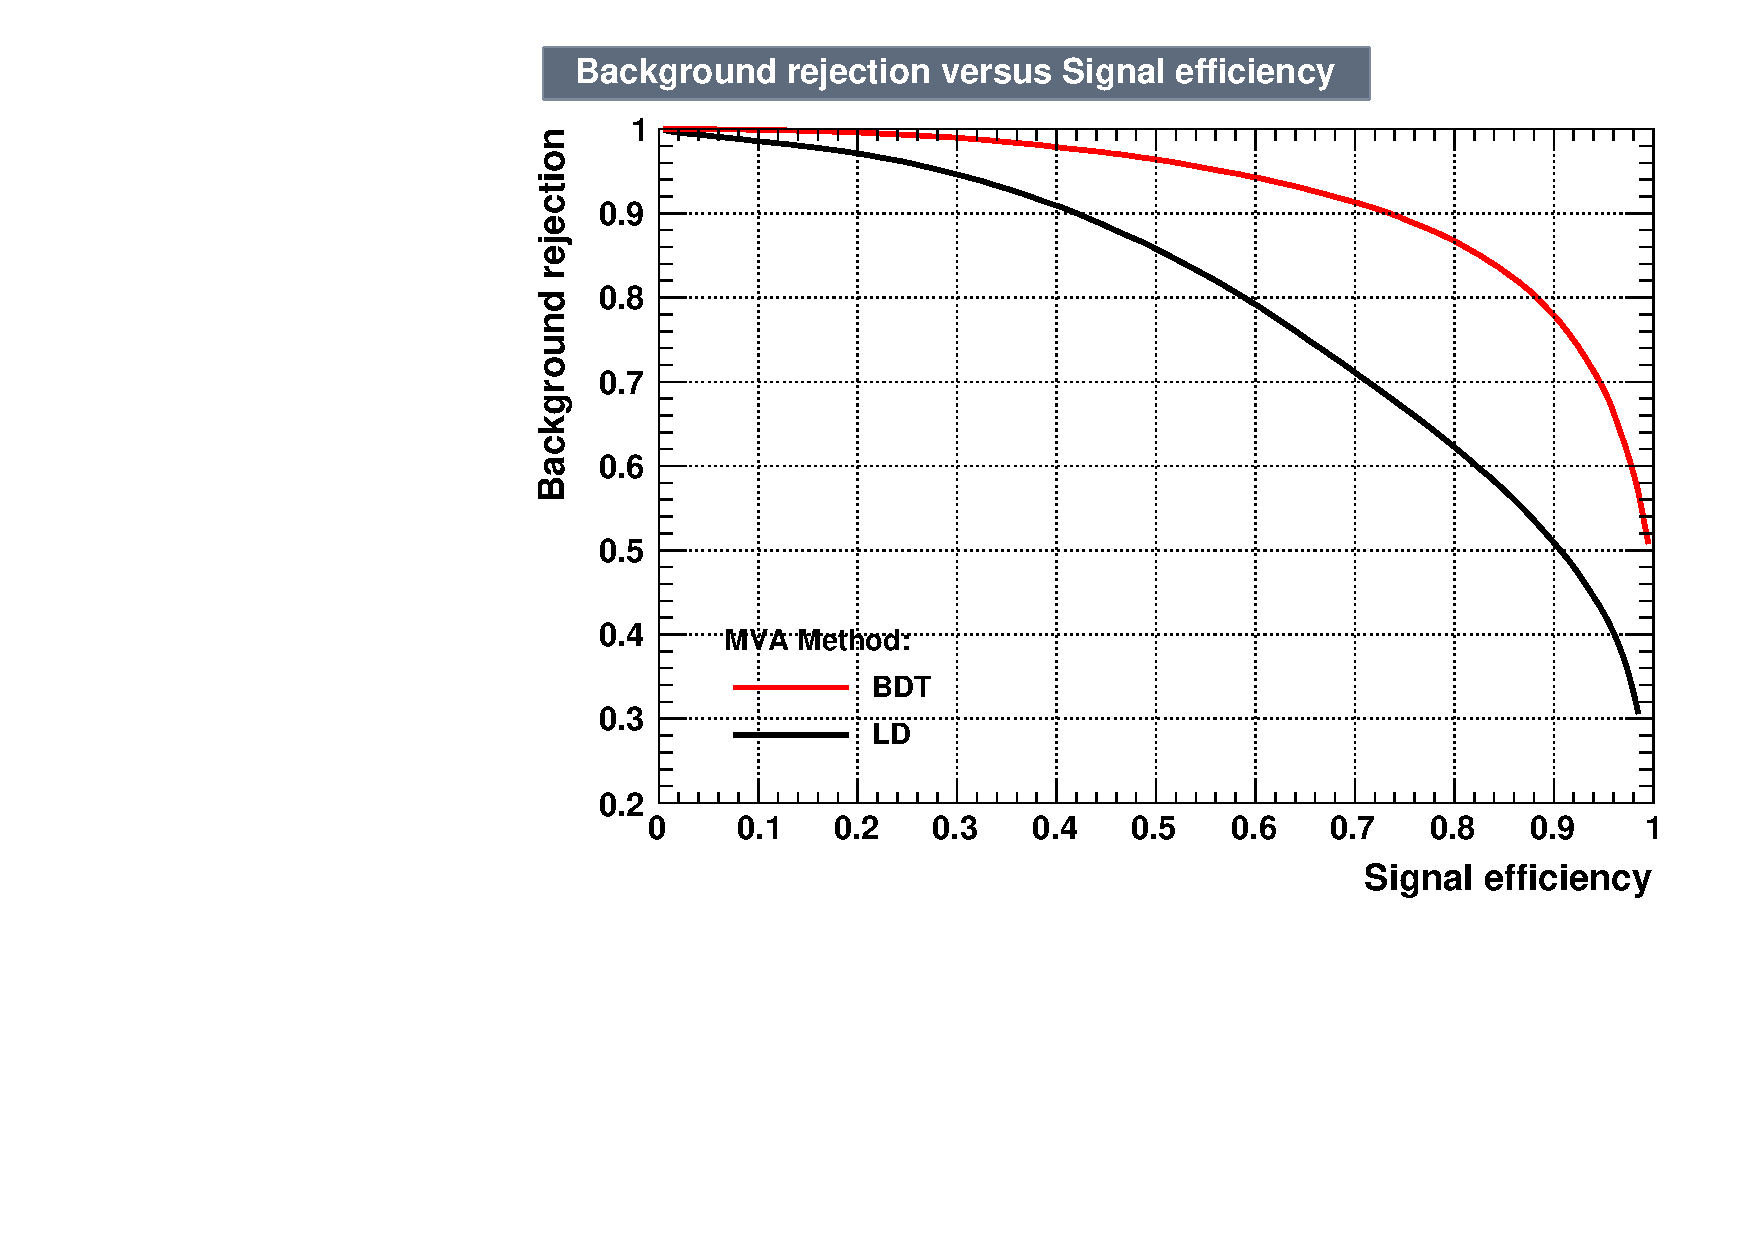
\includegraphics[width=0.75\textwidth]{bdtPlots_eles/low_roc.pdf}
   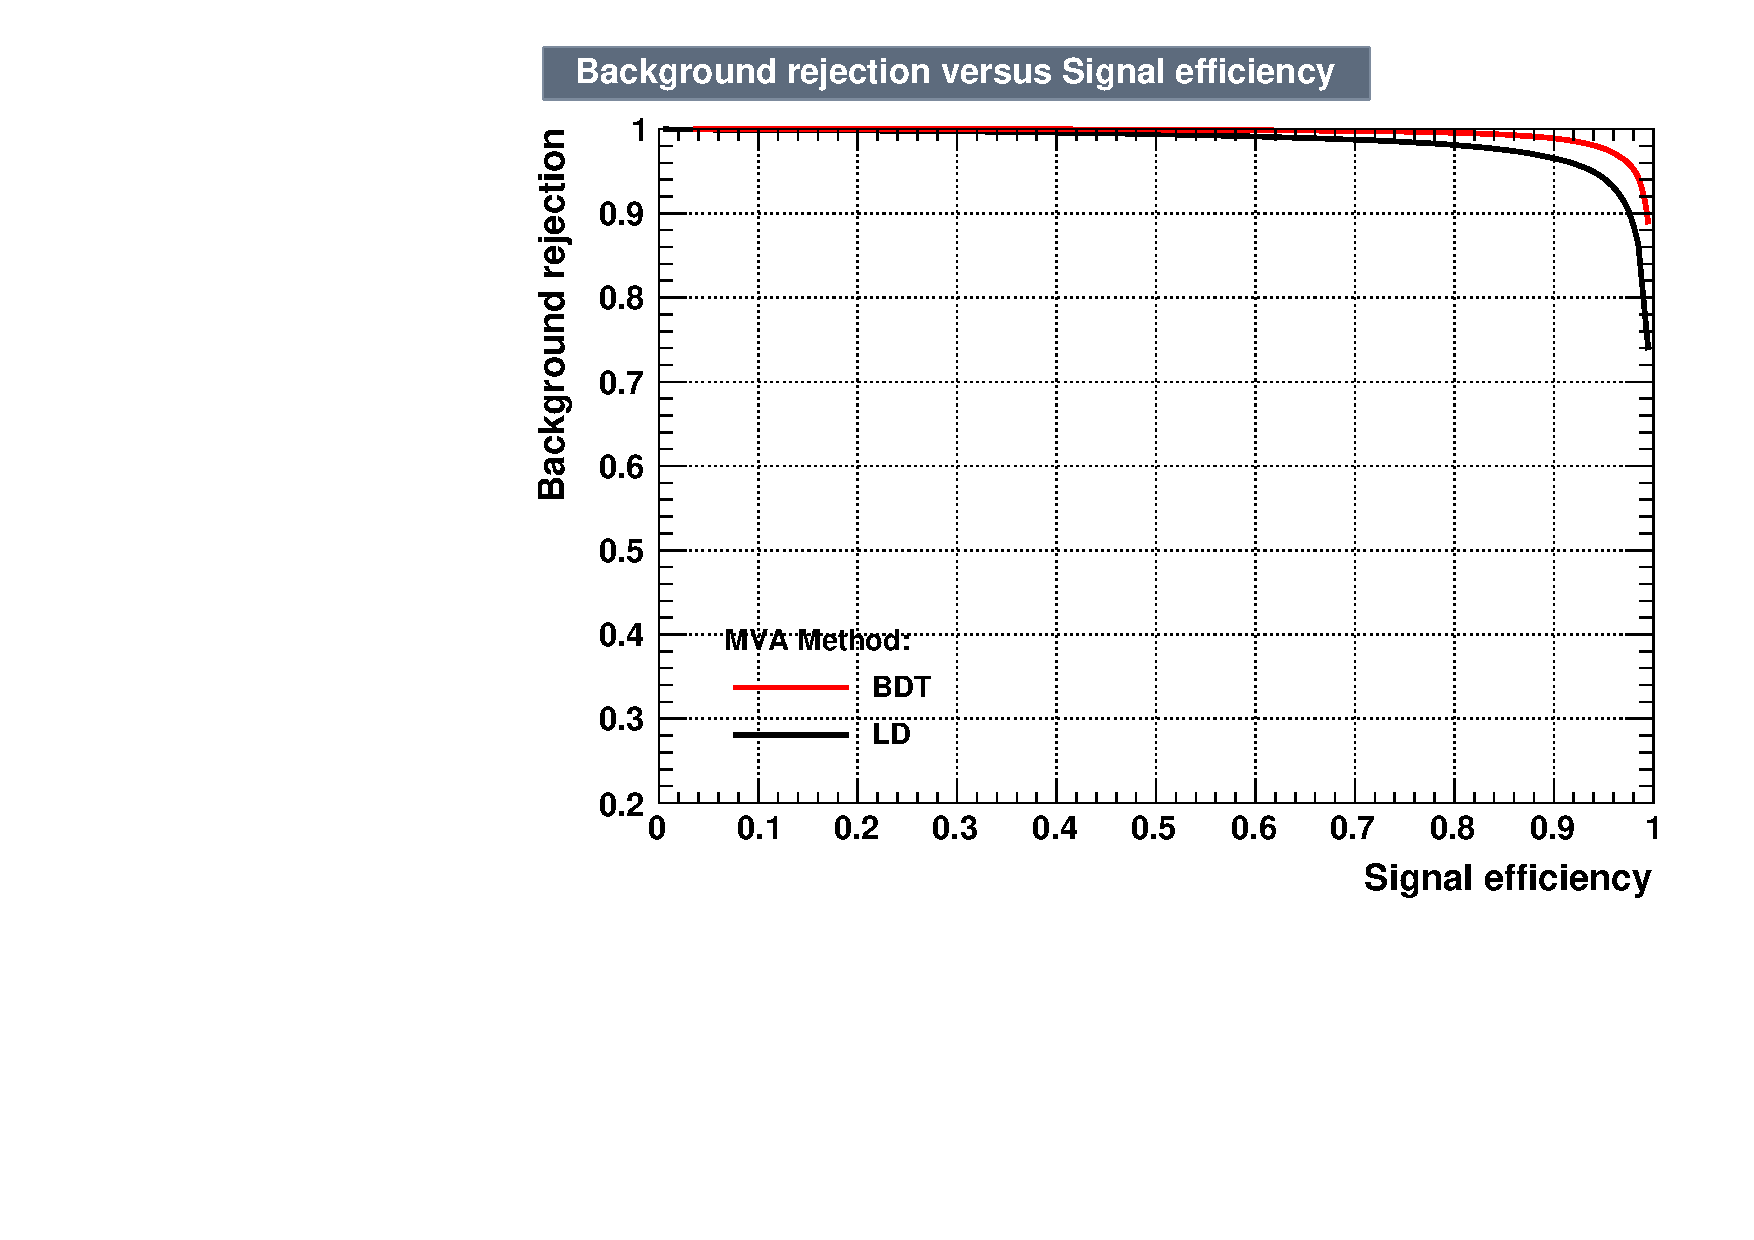
\includegraphics[width=0.75\textwidth]{bdtPlots_eles/high_roc.pdf}
    \caption{ ROC curves for electron channel. Top: low mass training. Bottom: high mass training. }
    \label{fig:ele_ROCs}
  \end{center}
\end{figure}

\begin{figure}[tbp]
  \begin{center}
   \includegraphics[width=0.75\textwidth]{bdtPlots_eles/low_corS.pdf}
   \includegraphics[width=0.75\textwidth]{bdtPlots_eles/low_corB.pdf}
    \caption{ Input variables correlations for electron channel, low mass training. Top: signal sample mix. Bottom: background sample mix. }
    \label{fig:ele_cors_low}
  \end{center}
\end{figure}


\begin{figure}[tbp]
  \begin{center}
   \includegraphics[width=0.75\textwidth]{bdtPlots_eles/high_corS.pdf}
   \includegraphics[width=0.75\textwidth]{bdtPlots_eles/high_corB.pdf}
    \caption{ Input variables correlations for electron channel, high mass training. Top: signal sample mix. Bottom: background sample mix. }
    \label{fig:ele_cors_high}
  \end{center}
\end{figure}


For completeness purpose and research reproducibility, it is worth mentioning in this paragraph the technical details. The following TMVA specific parameters have been used for the BDT training (most parameters are default ones since no significant improvement was observed when varying the parameters one at a time): NTrees = 800, BoostType=Grad, Shrinkage=0.1, UseBaggedBoost=True, GradBaggingFraction=0.5, SeparationType= GiniIndex, nCuts=30, and MaxDepth=3. %Few modifications did not improve much the performance.


Electrons and muons have been optimised separately but BDT trainings show similar performance (Fig. ~\ref{fig:ele_ROCs} and ~\ref{fig:muon_ROCs}). BDT distributions for data and MC comparison are created with the nominal values for the lepton and b jet scale factors. When shape systematics is considered to produce final limits, BDT shapes are
varied using 'Up' or 'Down' versions of the scale factors and all the input variables to the BDT are modified in the similar fashion as well. The BDT plots shown below are further modified applying postfit values of DY and \ttbar normalizations returned from the Maximum Likelihood fit performed with the real data. 



%% \begin{figure}[tbp]
%%   \begin{center}
%%    \includegraphics[width=0.35\textwidth]{low_muon.png}
%%    \includegraphics[width=0.35\textwidth]{high_muon.png}
%%     \caption{ Ranking of variables in the BDT training for muon channel. Left: low mass BDT. Right: high mass BDT.}
%%     \label{fig:muon_ranking}
%%   \end{center}
%% \end{figure}



\begin{figure}[tbp]
  \begin{center}
   \includegraphics[width=0.95\textwidth]{bdtPlots_muons/low_vars1.pdf}
   \includegraphics[width=0.95\textwidth]{bdtPlots_muons/low_vars2.pdf}
    \caption{Variables used in the low mass training for muon channel. Index '1' refers to \bbbar and index '0' refers to ZZ.}
    \label{fig:muon_lowVars}
  \end{center}
\end{figure}



\begin{figure}[tbp]
  \begin{center}
   \includegraphics[width=0.95\textwidth]{bdtPlots_muons/high_vars1.pdf}
   \includegraphics[width=0.95\textwidth]{bdtPlots_muons/high_vars2.pdf}
    \caption{ Variables used in the high mass training for muon channel.}
    \label{fig:muon_highVars}
  \end{center}
\end{figure}


\begin{figure}[tbp]
  \begin{center}
   \includegraphics[width=0.75\textwidth]{bdtPlots_muons/low_bdt.pdf}
   \includegraphics[width=0.75\textwidth]{bdtPlots_muons/high_bdt.pdf}
    \caption{ BDT discriminants for muon channel. Top: low mass training. Bottom: high mass training. }
    \label{fig:muon_BDTs}
  \end{center}
\end{figure}

\begin{figure}[tbp]
  \begin{center}
   \includegraphics[width=0.75\textwidth]{bdtPlots_muons/low_roc.pdf}
   \includegraphics[width=0.75\textwidth]{bdtPlots_muons/high_roc.pdf}
    \caption{ ROC curves for muon channel. Top: low mass training. Bottom: high mass training. }
    \label{fig:muon_ROCs}
  \end{center}
\end{figure}

\begin{figure}[tbp]
  \begin{center}
   \includegraphics[width=0.75\textwidth]{bdtPlots_muons/low_corS.pdf}
   \includegraphics[width=0.75\textwidth]{bdtPlots_muons/low_corB.pdf}
    \caption{ Input variables correlations for muon channel, low mass training. Top: signal sample mix. Bottom: background sample mix. }
    \label{fig:muon_cors_low}
  \end{center}
\end{figure}


\begin{figure}[tbp]
  \begin{center}
   \includegraphics[width=0.75\textwidth]{bdtPlots_muons/high_corS.pdf}
   \includegraphics[width=0.75\textwidth]{bdtPlots_muons/high_corB.pdf}
    \caption{ Input variables correlations for muon channel, high mass training. Top: signal sample mix. Bottom: background sample mix. }
    \label{fig:muon_cors_high}
  \end{center}
\end{figure}



\section{Systematic Uncertainties}
\label{sec:Systematics}

Systematic uncertainties that affect the sensitivity of our di-Higgs search
come from a variety of sources such as theoretical uncertainties on
cross sections or proton structure, experimental uncertainties related
to the modelling of the detector response, the amount of collected
data, and the discrepancies between the simulated samples and the real data.

Systematic uncertainties can be divided into two broad categories:
those affecting only the yields of selected events from different processes
(the "normalization" uncertainties) and those that, in addition to the change in rate, may
distort the shape of the \mTHH distribution used in the extraction of
the limits (the "shape" uncertainties). %Systematic uncertainties of all types enter the likelihood function of the fit in the limits extraction as independent nuisance parameters.                                                                                                                                                                                                                                                                                                                                                                                                                                                                                                                                                                     

\subsection{Normalization uncertainties}

%Normalization uncertainty for each source of the systematic bias is determined through variation of parameters governing the impact of that bias and measuring the effect of such variation on the yield of signal and background components of the sample. The size of the effect then enters the likelihood fit as a constraint on the corresponding nuisance parameters.                                                                                                                                                                                                                                                                                                                                                                             

The sources of systematic
uncertainties that affect normalizations are discussed in the list below. The sizes of some
systematic uncertainties may vary depending on the resonance mass hypothesis
and the decay channel of the leptonically decaying \PZ boson, in which cases
ranges of the uncertainty values are listed. Normalization uncertainties
discussed in this section do not affect the normalizations of the \ttbar and DY
backgrounds because those are determined from data during the simultaneous fit of the signal and control regions.

\begin{itemize}

\item{\bfseries Luminosity} - CMS estimated this uncertainty on the integrated
  luminosity of the CMS 2016 data set to be $2.5\%$
  ~\cite{CMS-PAS-LUM-17-001}. This uncertainty directly affects the
  expected event yields for the signal processes as well as all
  background processes except for the two dominant backgrounds, DY and
  \ttbar. %, which have their normalization determined in the limits extraction likelihood fit.

\item{\bfseries Pileup} - Signal and background event yields depend on the
  accuracy of the reproduction of pileup interactions in each simulated event. The effect of pileup is considered on each process. The recommended nominal value of 69.2 mb is used for the total inelastic pp cross section, for Down and Up variations, the values of 66.02 and 72.38 mb are used respectively, reflecting the imperfect knowledge of the total inelastic
  proton-proton interaction cross section at 13~TeV. The effect is seen only in the normalization and we, thus, consider this a normalization uncertainty and assign the value of $6\%$.

\item{\bfseries Proton PDF} - The systematic bias associated with the limited
  knowledge of the interacting proton content is evaluated using an ensemble of a hundred of PDF
  replicas from the NNPDF set \cite{Ball:2014uwa} following the
  PDF4LHC prescription \cite{Botje:2011sn,Alekhin:2011sk} and the RMS
  of the resulting process normalizations is taken as a measure of the
  bias. It is found to be of order 5\%.

\item{\bfseries QCD scales} - Theoretical uncertainties in the QCD
  factorization and renormalization scales affect the expected yield
  of the signal and background events, excluding the \ttbar and DY
  yields as mentioned earlier. This uncertainty is estimated
  by varying independently these two scales in simulation by factors 0.5 and 2 with respect to the nominal
  values of the scales. The unphysical cases with one of the scales
  fluctuating up while the other fluctuates down are discarded. In
  each bin of the HH transverse mass distribution the maximum and
  minimum variation are used to build an envelope around the nominal
  shape, resulting in the effect of the size 4-6\% on the processes' yields.

%\item{\bfseries Theoretical cross sections} - The theoretical cross section is  used to normalize the contribution from the single top  background. The uncertainty in this cross section is propagated to  the uncertainty in the background yields for this process and is   found to be 5--7\%.

% \item {\bfseries MET}: the effect of the JEC and JER on the MET is studied modifying MET variables that go into HH transverse mass shape used in the final fit. The effect of the calibration of unclustered MET, meaning missing energy associated with particles that are not clustered into jets, is found only on the normalization, the shape itself is not distorted. The size of the effect is $~3\%$ depending on the mass hypothesis and the $3\%$ normalization uncertainty is used in the analysis.
%

\item{\bfseries Missing transverse energy/momentum} - Clustered energy in
  jets and leptons undergo energy corrections during event
  reconstruction, however, neutral hadrons and photons that do not belong to any jet
  ("unclustered energy") and jets with low transverse momenta (below
  10~GeV) lack such corrections. This results in a small systematic
  bias in the reconstructed missing transverse momentum. \ETslash enters the \mTHH variable, thus the effect of the unclustered energy has to be studied. We shift the energy of each
  particle not contained in jets or contained in low-\pt jets by its
  uncertainty Up and Down. Such variations affect the event yields of signal and background processes at about
  3\% level but do not have a visible effect on the shape of the HH
  transverse mass, thus this source is categorised as a
  "normalization" systematic source.

\end{itemize}



\subsection{Shape uncertainties}

Several sources of systematic uncertainties affect not only the rate but also the shapes of various
kinematic distributions which are inputs to the BDT or a part of the \mTHH construction, the BDT discriminant itself, and the shape of the \mTHH distribution. Each source is varied separately within one standard deviation up and down, and
the effect is propagated through all related variables resulting in
the nominal shape of the HH invariant mass distribution and two
modified shapes corresponding to the Up and Down variations. Such triplet of shapes is prepared for each channel, each mass hypothesis, and for all processes. %both for the signal and control regions of the kinematic phase space.                                                                                                                                                                                                                                                                                                                                                                                                                                                                                                                                                                                       

All these shapes are fit simultaneously in the
signal extraction likelihood fit. The discussion of the these sources
of uncertainties follows.



\begin{itemize}

\item{\bfseries Lepton efficiency} - The effect of the detector on the reconstruction of the lepton: identification and isolation selection
  criteria, and the requirement to pass trigger selection requirements are studied separately and are used to account for data/MC discrepancies. The corrections are derived
  from large dedicated samples of \PZ boson decays and also have an error associated with the procedure. 
  %are themselves known with limited accuracy. 
  The uncertainty on lepton efficiency corrections are derived
  as a function of lepton $p_T$ and $\eta$ and is propagated to the final \mTHH distributions.
  The effect of these uncertainties is sub-percent for the muon
  channel and up to 6\% for the electron channel.


\item{\bfseries Jet energy scale} - The uncertainty on the jet energy scale
  affects \HBB mass and \pt, which are inputs to the BDT. In addition, jet energy scale directly affects \HBB mass and \ETslash, which are used during the construction of the HH invariant mass. %Several factors affecting the calibration of the jet energy scale are considered independently as they are uncorrelated. 
  Jet energy scale is varied Up and Down within one standard deviation of its uncertainty %for each of these factors 
  as a function of jet $p_T$ and $\eta$, and the
  effect on the jet kinematics and on the \ETslash is calculated and
  propagated through the steps of the measurement yielding the
  variation of the HH invariant mass shape.  Jet energy scale
  uncertainty, with all factors combined, has the effect on the yields
  of the signal and some background components as large as 5 to 10\%.

\item{\bfseries Jet energy resolution} - Data and MC a different energy
  resolution, which also affects the final \mTHH shapes via its effect on the dijet invariant
  mass for \HBB and its effect on the \ETslash. Jet energy resolution
  is varied in simulation by one standard deviation as a function of
  jet $p_T$ and $\eta$ and the effect is propagated through the steps
  of the measurement. Its effect on the \mTHH yield is typically order of 0.5\%.

\item{\bfseries b-tagging and mistagging} - The efficiency to tag a \Pqb-jet and the
  probability to misidentify a different flavor or a gluon jet and tag it as a
  \Pqb-jet is corrected in MC samples by factors derived from
  flavor-enhanced jet samples. The uncertainties on these corrections
  are propagated through the whole analysis setup. The effect of the
  \Pqb-tagging efficiency (mistagging/flavor misidentification) is about 5\% (7--10\%) for the Drell-Yan process and at the sub-percent level for other processes (7--10\%).
% to  about 5\% for the Drell-Yan process, while the flavor misidentification impact is larger and is seen to be in the range 7--10\% for most processes.                                                                                                                                                                                                                                                                                                                                                                                                                                                                                                                                                                                                

\item{\bfseries Bin-by-bin uncertainties} - Since the available statistics for the simulated MC samples is limited, the lack of events in some bins of the \mTHH distribution is addressed by bin-by-bin (BBB) uncertainty. This effect may result in sizeable fluctuations of the bin content of the HH invariant mass shapes that enter the
  likelihood fit. Therefore, for each bin of the HH invariant mass distributions
  an individual nuisance parameter is added to the likelihood fit with the Gaussian constraint of one standard deviation of
  the yield uncertainty in that bin.
  
\end{itemize}







%\begin{sidewaystable}
%\begin{center}
%\caption{Yield variations, ee channel, 300 GeV.}
%\begin{tabular}{ | c | c | c | c | c | c |c | c | } \hline
% sample & b-tagging &  mistag &  electron IDnISO &  electron tracker &  electron trigger &  jet resolution &  jet scale \\\hline
%  DY &              4.3 &     7.4 &              5.4 &               1.1 &               2.1 &             0.2 &        5.3 \\
%  TT &              0.5 &     7.4 &              4.7 &               1.1 &               1.9 &             0.0 &        0.5 \\
%  signal\_bbzz &    0.2 &     7.6 &              5.0 &               1.1 &               2.0 &             0.7 &        5.8 \\
%  signal\_bbww &    0.0 &     7.6 &              6.7 &               1.1 &               2.9 &             0.0 &        1.6 \\\hline
%\end{tabular}
%\label{normalization_electron}
%\end{center}
%%---------------------------------------------------------------------                                        
%%Vertical lines as column separators                                                                          
%\begin{center}
%\caption{Yield variations, mm channel, 300 GeV.}
%\begin{tabular}{ | c | c | c | c| c | c | c | c| c |}\hline
%sample &  b-tagging &  mistag &  muon ID &  muon ISO &  muon tracker &  muon trigger &  jet resolution &  jet scale \\\hline
%  DY &              4.9 &     7.0 &      0.2 &       0.1 &           0.1 &           0.4 &             0.2 &        9.4 \\
%  TT &              0.9 &     7.2 &      0.2 &       0.1 &           0.0 &           0.4 &             0.6 &        0.7 \\
%  signal\_bbzz &    0.3 &     7.7 &      0.2 &       0.1 &           0.0 &           0.4 &             0.5 &        4.4 \\
%  signal\_bbww &    0.0 &     9.2 &      0.2 &       0.1 &           0.0 &           0.1 &             0.0 &        8.5 \\\hline
%\end{tabular}
%\label{yieldVariations}
%\end{center}
%%\end{table}
%\end{sidewaystable}
%\begin{sidewaystable}
%\begin{center}
%\caption{Yield variations, ee channel, 300 GeV.}
%\begin{tabular}{ | c | c | c | c | c | c |c | c | } \hline
% sample & b-tagging &  mistag &  electron IDnISO &  electron tracker &  electron trigger &  jet resolution &  jet scale \\\hline
%  DY &              4.3 &     7.4 &              5.4 &               1.1 &               2.1 &             0.2 &        5.3 \\
%  TT &              0.5 &     7.4 &              4.7 &               1.1 &               1.9 &             0.0 &        0.5 \\
%  signal\_bbzz &    0.2 &     7.6 &              5.0 &               1.1 &               2.0 &             0.7 &        5.8 \\
%  signal\_bbww &    0.0 &     7.6 &              6.7 &               1.1 &               2.9 &             0.0 &        1.6 \\\hline
%\end{tabular}
%\label{normalization_electron}
%\end{center}
%%---------------------------------------------------------------------                                        
%%Vertical lines as column separators                                                                          
%\begin{center}
%\caption{Yield variations, mm channel, 300 GeV.}
%\begin{tabular}{ | c | c | c | c| c | c | c | c| c |}\hline
%sample &  b-tagging &  mistag &  muon ID &  muon ISO &  muon tracker &  muon trigger &  jet resolution &  jet scale \\\hline
%  DY &              4.9 &     7.0 &      0.2 &       0.1 &           0.1 &           0.4 &             0.2 &        9.4 \\
%  TT &              0.9 &     7.2 &      0.2 &       0.1 &           0.0 &           0.4 &             0.6 &        0.7 \\
%  signal\_bbzz &    0.3 &     7.7 &      0.2 &       0.1 &           0.0 &           0.4 &             0.5 &        4.4 \\
%  signal\_bbww &    0.0 &     9.2 &      0.2 &       0.1 &           0.0 &           0.1 &             0.0 &        8.5 \\\hline
%\end{tabular}
%\label{yieldVariations}
%\end{center}
%%\end{table}
%\end{sidewaystable}
%\begin{sidewaystable}
%\begin{center}
%\caption{Yield variations, ee channel, 300 GeV.}
%\begin{tabular}{ | c | c | c | c | c | c |c | c | } \hline
% sample & b-tagging &  mistag &  electron IDnISO &  electron tracker &  electron trigger &  jet resolution &  jet scale \\\hline
%  DY &              4.3 &     7.4 &              5.4 &               1.1 &               2.1 &             0.2 &        5.3 \\
%  TT &              0.5 &     7.4 &              4.7 &               1.1 &               1.9 &             0.0 &        0.5 \\
%  signal\_bbzz &    0.2 &     7.6 &              5.0 &               1.1 &               2.0 &             0.7 &        5.8 \\
%  signal\_bbww &    0.0 &     7.6 &              6.7 &               1.1 &               2.9 &             0.0 &        1.6 \\\hline
%\end{tabular}
%\label{normalization_electron}
%\end{center}
%%---------------------------------------------------------------------                                        
%%Vertical lines as column separators                                                                          
%\begin{center}
%\caption{Yield variations, mm channel, 300 GeV.}
%\begin{tabular}{ | c | c | c | c| c | c | c | c| c |}\hline
%sample &  b-tagging &  mistag &  muon ID &  muon ISO &  muon tracker &  muon trigger &  jet resolution &  jet scale \\\hline
%  DY &              4.9 &     7.0 &      0.2 &       0.1 &           0.1 &           0.4 &             0.2 &        9.4 \\
%  TT &              0.9 &     7.2 &      0.2 &       0.1 &           0.0 &           0.4 &             0.6 &        0.7 \\
%  signal\_bbzz &    0.3 &     7.7 &      0.2 &       0.1 &           0.0 &           0.4 &             0.5 &        4.4 \\
%  signal\_bbww &    0.0 &     9.2 &      0.2 &       0.1 &           0.0 &           0.1 &             0.0 &        8.5 \\\hline
%\end{tabular}
%\label{yieldVariations}
%\end{center}
%%\end{table}
%\end{sidewaystable}













%
%
%Systematic uncertainties may change the derived limits. Uncertainties
%that we consider may change the normalization or distort the shape
%that we used for fits. The following sources of the uncertainties have
%been included:
%\begin{itemize}
%
% \item {\bfseries Luminosity}: an uncertainty of $2.5\%$ is assigned for
%   2016 luminosity. All the processes are affected except those, which normalization is determined using data driven methods: DY and \ttbar normalization
%
% \item {\bfseries Lepton Efficiency}: identification, isolation, tracker,
%   and trigger scale factors have been determined using the standard EGamma POG and Muon POG technique of the Tag-and-Probe. 
%   Up and Down variations with respect to the nominal value of the scale factor (within the uncertainty on the value) have been propagated to the final HH transverse mass shape that goes to the fit with the Higgs Combination Tool. Each scale factor type (identification, isolation, tracker,
%   and trigger scale factor) is propagated independently. Overall, the effect of the lepton efficiency, when dealing with b jets, is a very minor
%   one.  These uncertainties are included in both electron and muon channels.
%
% \item {\bfseries MET}: the effect of the JEC and JER on the MET is studied modifying MET variables that go into HH transverse mass shape used in the final fit. The effect of the calibration of unclustered MET, meaning missing energy associated with particles that are not clustered into jets, is found only on the normalization, the shape itself is not distorted. The size of the effect is $~3\%$ depending on the mass hypothesis and the $3\%$ normalization uncertainty is used in the analysis.
%
% \item {\bfseries Jet Energy Scale}: following JetMET group recommendation we check the effect of this uncertainty
%   on all jet-related variables that enter BDT and/or HH system. The scale value is varied Up and Down and modified HH
%   transverse mass shapes are obtained and used in the final fit.
%
% \item {\bfseries Jet Energy Resolution}: we vary up and down jet energy
%   resolution by one $\sigma$ and modify all the jet related
%   variables that are a part of the BDT and/or HH system prior to constructing the final shape. Varied HH transverse mass shapes are used in the final fit.
%
% \item {\bfseries B-jet Tagging and mistag uncertainties}: following the suggestions from the BTV POG
%   b tag and mistag scale factors are applied to all MC samples. The effect of the usage of 
%   light and heavy flavor scale factors is propagated to the final shapes.
%
% %% \item {\bfseries PDF uncertainties}: impossibility to know precisely the
% %%   content of the colliding proton or gluon is addressed in this
% %%   uncertainty. Using the recommended values from LHC Higgs Cross Section group documented in the CERNYellowReportPageAt13TeV we assign $O(1-5)\%$ uncertainties to quark-quark initiated
% %%   processes and $O(10-20)\%$ uncertainties to gluon-gluon uncertainties depending on the process.
%  
% %% \item {\bfseries QCD scale variations}: The uncertainty on the QCD normalization scale for each
% %%   individual process is assigned to a corresponding specific theory error suggested by CMS generator group, which maintains a twiki page with a collection of cross sections for Standard Model processes to be used in the CMS analyses. More information on how the cross-sections and the associated theory errors have been determined is available at ~\cite{SMxsec}. 
%
%\item {\bfseries QCD scale variations}: This uncertainty is estimated by varying the renormalization ($\mu_{R}$) and the factorization ($\mu_{F}$) scales, independently by a factor of 2, meaning from the nominal value of 1 to values of 0.5 and 2. Unphysical situations with one scale fluctuating up and the other fluctuating down are not considered. In each bin of the distribution the maximum (minimum) variation is used as an estimate of the QCD scale uncertainties for all the background and signal samples. The resulting effect has been found on the normalization at the order of $4-6\%$.
%
%
%\item {\bfseries PDF uncertainties}: impossibility to know precisely the
%   content of the colliding proton or gluon is addressed in this
%   uncertainty. The RMS of each of the 101 NNPDF MC variations of the strong coupling constant for each simulated background and signal processes is calculated and the largest one is assigned as a normalization uncertainty, and is of the order of $5\%$. 
%
%
%
%
%
%%% \item {\bfseries PDF uncertainties}: impossibility to know precisely the
%%%    content of the colliding proton or gluon is addressed in this
%%%    uncertainty. For each process, the RMS of each of the 101 NNPDF MC variations is calculated and the largest one is assigned as a normalization un\
%%% certainty, and is of the order of $5\%$.
%
%%%  \item {\bfseries QCD scale variations}: The QCD scale normalization and factorization at $1/2$ and 2 have been applied to each sample and the resulting e\
%%% ffect has been found to be $4-6\%$.
%
%
%
%
%
% %\item {\bfseries Cross section normalization}: Uncertainty associated with the cross section value for the
%   %\ttbar and single top processes. We used the same numbers as in bbVV analysis.
%
% \item {\bfseries Pile up }: The effect of pile up on each
%   process is considered. The recommended nominal value of 69.2 mb is used for the total inelastic pp cross section, for Down and Up variations, the values of 66.02 and 72.38 mb are used respectively. The effect is seen only in the normalization and we, thus, switch to the normalization uncertainty and assign the value of $6\%$.
%
%
% \item {\bfseries Drell-Yan and \ttbar normalizations }: \ttbar and Drell-Yan
%   normalizations we extract from the simultaneous fit of both signal
%   region and DY and \ttbar ~control regions. Normalizations of main backgrounds are allowed to float freely to let the fitter find the best values of the DY and \ttbar normalizations to fit the existing data. HH transverse mass distributions are used in the fit. Separately, an option of control regions only fit has been studied and results were found consistent with the DY and \ttbar normalizations obtained from the fit where signal region was included. Overall, the normalization of \ttbar is near the value
%   '1', deviating up to $\approx10-20\%$ depending on the mass point. DY normalization is deviating higher from the value of '1' since the requirement on 2 b jets and a high boost pushes DY process to higher pT and flavor phase space that is not well modeled in the MC. Therefore, a part of the analysis strategy was to extract these numbers using the real data. The final $\chi^2$ values after the application of \ttbar and Drell-Yan normalizations are near the value '1'.
%
% \item {\bfseries Bin-by-bin uncertainties } To account for the low statistics in some bins of HH transverse mass distribution in MC, bin-by-bin uncertainties should be used. If the error on the MC in the bin is zero, the bin is skipped entirely. However, if the error is non zero and if the number of effective events for each given process is lower than or equal to zero, a Poisson-constrained parameter will be created. Otherwise a Gaussian-constrained parameter is assigned to this bin. Barlow-Beeston algorithm is used to create these bin-by-bin parameters which scale the total yield in the bin. The advantage of this algorithm is that each nuisance parameter has a simple analytic form and analytic minimization can be performed, which results in the reduction of the fit time and an increase of the fit stability.
%
% \item {\bfseries Shape uncertainties}: All shape systematic
%   uncertainties are addressed separately and all together are used in the final fit. The following uncertainties are considered as shape
%   uncertainties: each of lepton scale factors, b tag scale factors of
%   both light and heavy flavour, effect of JEC and JER on all the variables used in
%   BDT and/or HH system. For all these shape uncertainties we
%   propagate the source of uncertainty through all the related
%   variables that enter our BDT or region selection all the way to
%   building the HH candidate and obtaining the final shape.  We
%   produce, therefore, final shapes with the 'nominal value' as well
%   as with 1~$\sigma$ 'Up' and 'Down' variations. 
%
%\end{itemize}


%% \begin{center}
%% \begin{figure}[tbp]
%% %\includegraphics[width=0.5\textheight]{impacts_nov7_300GeV.pdf}
%% %\caption{ Impacts plot for 300 GeV case. Actual limit at this mass point is $248.25_{-71.07}^{+103.9}$~pb.}
%% %\includegraphics[width=0.5\textheight]{impacts_april6.pdf}
%% \includegraphics[width=0.5\textheight]{impacts_50_strategy2_july23_300.pdf}
%% \includegraphics[width=0.5\textheight]{impacts_1500_strategy0_july23_900.pdf}
%% \caption{ Impacts plot for 300(top) and 900 (bottom) GeV case.}% Actual limit at this mass point is $248.25_{-71.07}^{+103.9}$~pb.}
%% \label{fig:impactsBBB}
%% \end{figure}
%% \end{center}



%Following the Higgs PAG list of question for the preapproval checks ~\cite{HiggsPAGPreapprovalChecks}, we produce for 300 GeV case fit results for a background-only Asimov toy (Fig.~\ref{mlfit_Asimov}) and a signal+background Asimov toy (Fig.~\ref{mlfit_Asimov}), with the corresponding outputs of running "diffNuisances.py" that can be found at ~\cite{Comparison_of_nuisances_expectedSignal0_350} and ~\cite{Comparison_of_nuisances_expectedSignal1_350}. 





%\begin{table}


%The impacts plot with BBB uncertainties can be found at Fig.\ref{fig:impactsBBB}.%~\ref{pulls}.




%\section{Results}
%\label{sec:results}
\section{Statistical Analysis}
\label{sec:statistics}


The results in this measurement are obtained with the maximum likelihood fit. We perform a simultaneous fit of the SR and both CRs for both dielectron and dimuon channels using the likelihood function constructed as a product
of Poisson terms over all bins of the input \mTHH distributions in the three regions (SR, CRDY, CRTT) with Gaussian terms to constrain the nuisance parameters:

\begin{align*}
 L(r_{\text{signal}}, r_{k}|\text{data}) = \prod_{i=1}^{N_{\mathrm{bins}}}\frac{\mu_{i}^{n_{i}}\cdot e^{-\mu_{i}}}{n_{i}!}
\cdot \prod_{j=1}^{N_{\mathrm{nuisances}}} e^{-\frac{1}{2}\theta_{j}^{2}}
\end{align*}

\noindent where the product index $i$ refers to the bin of the input distributions, the product index $j$
refers to uncertainties accounted for by the fit model, and $n_i$ is the number of observed data
events in the bin $i$. The mean value for each of the Poisson distributions is computed as:


\begin{align*}
\mu_{i} &= r_{\text{signal}} \cdot S_{i} + \sum_{k}r_{k}\cdot B_{k,i},
\end{align*}


\noindent where $k$ refers to the background process $k$, and $B_{k,i}$ is the content of the bin $i$ of the background
shape for a process $k$, while $S_i$ is the content of the bin $i$ of the signal shape. The parameter $r_k$
sets the normalization of the background process $k$ while $r_{signal}$ is the signal strength parameter, all $r$ parameters are floating freely in the fit.
Two values of the signal strength parameter are of special interest:  $r_{signal} = 0$ describes the
background-only hypothesis, while $r_{signal} = 1$ corresponds to the case when the HH cross section
matches the cross section used for the initial signal normalization inspired by BSM models, 2pb in our case. 
The terms $\theta_j$ represent the set of nuisance parameters that are introduced into the likelihood
function as Gaussian constraints. 


Figure~\ref{fig:MCcomparisons}(~\ref{fig:MCcomparisons_radion}) shows the HH transverse mass distributions
for the signal and two control regions for both channels for the graviton (radion) resonance mass hypothesis with normalizations and shapes of all
components adjusted according to the best-fit values. The signal
sample is normalized to the cross section of 2~pb, a typical value for
predictions of WED models (e.g., at 300 GeV), and is further scaled, as indicated on the
Figure, to make it clearly visible. %The distributions exhibit a good agreement between data and the sum of the backgrounds.                                                                                                                                                                                                                                                                                                                                                                                                                                                                                                                                                                                                                                                                                                                                                                                




With the given 2016 dataset, the fit results show no evidence for HH production through a narrow
resonance, whose width is negligible in comparison to experimental
resolution, in the mass range from 250~GeV to 1~TeV. Thus, upper 95 \% confidence level limits on the
HH production cross section are set using the modified
frequentist CL$_s$ approach (asymptotic CL$_s$)~\cite{Junk:1999kv,LEP-CLs, HIG-11-011, Cowan:2010js}.

The observed and expected 95\% upper CL limits for the full mass range
and both resonances are listed in Table~\ref{tab:finalLimits}. We produce the standard CMS Brazilian-flag type of plot for the limits, shown in Fig.~\ref{fig:HHlimits}. The green and yellow
bands correspond to one and two standard deviations around
the expected limit respectively. Since 450 GeV is the separation boundary between two mass regions: low mass and high mass, the limit calculation is performed with both of the BDTs at 450 GeV, where the discontinuity is
seen in the figure. The Figure also shows the expected production
cross section for a RS1 KK graviton/RS1 radion in WED models. %For a scenario with the curvature parameter $k/\overline{M}_{Pl}=0.1$ and the size of the extra dimension $kL=35$.                                                                                                                                                                                                                                                                                                                                                                                                                                                                                                                                                                                                                                                                                                                           
This cross section is computed in \cite{Oliveira:2014kla}
under the assumption of no mixing with the SM Higgs boson.











\section{Limits Extraction}
\label{sec:limits}

Prior to the derivation of the expected limits, we had to make sure their values are the most sensitive limits that our analysis can set. For that, we have done an optimization study finding the best cut value on the BDT discriminant with the idea to yield the lowest (the most sensitive) limit. 



\subsection{Optimization for the best limit}

For this study, before doing the combination of electron and muon channels, we have optimized each of the channels separately. Systematical uncertainties were present only of the normalization type (lnN), since we are statistically limited and systematics plays a secondary role. %The latter can be seen running the fit with the "-S 0" option, which ignores systematics entirely. 
As an example, for a specific analysis setup the 300 GeV fit in the muon channel yields the limit ('r-value') 255.25 (with the systematics but neglecting BBB uncertainties), without systematics the 'r-value' is 238.25. The difference is 17 parts in 255.25, which is just 6.7 $\%$.

As can be seen from the plots ~\ref{fig:ele_bdt_vs_r} and ~\ref{fig:muon_bdt_vs_r}, for high mass region the best cut to use is 0.99 for both electron and muon channels. For low mass region, the situation is more complicated. Depending on the mass point (and channel!) one cut is better than the other. For electron channel for 400 and 450 GeV mass points the best cut is 0.925. In the lower region, the situation changes, 0.2 for 260 GeV, 0.4 for 270 and 300 GeV, 0.825 for 350 GeV. 

Running the whole analysis for each separate cut and channel and spin hypothesis is not possible computationally taking into account the number of samples and shapes one has to create and process. That is why a reasonable compromise is to observe that for 260 $\to$ 350 GeV included, the suboptimal cut can be 0.4, being well inside the $1\sigma$ error band. This leaves the whole mass range with just three different cut values. This approach of suboptimal cuts, cuts which are close the best values but, most importantly, can be shared among several mass points, is what we adopted for this measurement. 

For instance, for muons the best cuts are: 0.1 for 260 and 270 GeV, 0.5 for 300 GeV, 0.7 for 350 GeV, 0.925 for 400 and 450 GeV. Taking the approach of suboptimal cuts, the values we kept are: 0.1 for 260 and 270 GeV, 0.7 for 300 $\to$ 450 GeV included. This way we simplify the analysis to three different BDT cuts per channel and, at the same time, remain optimal within the error bands with respect to the best cut values. This is summarized in the Table~\ref{suboptCut}.

\begin{table}
\begin{center} 
  \caption{Suboptimal BDT cuts used in the analysis}
 \begin{tabular}{ |c|c|c|c|c| } \hline%\hline
   channel & 260 and 270 GeV & 300 and 350 GeV & 400 and 450 GeV & 600 GeV to 1000 GeV \\ \hline
   muons & 0.1 & 0.7 & 0.7 & 0.99 \\ %\hline
   electrons & 0.4 & 0.4 & 0.925 & 0.99\\ \hline%\hline
  \end{tabular}
  \label{suboptCut}
\end{center}   
\end{table}









\begin{figure}[!htb]%hbpt?        
\includegraphics[width=0.5\textwidth, height=0.2\textheight,  keepaspectratio]{eles_bdt_vs_r/gr_limits__260GeV.pdf}
\includegraphics[width=0.5\textwidth, height=0.2\textheight,  keepaspectratio]{eles_bdt_vs_r/gr_limits__270GeV.pdf}
\includegraphics[width=0.5\textwidth, height=0.2\textheight,  keepaspectratio]{eles_bdt_vs_r/gr_limits__300GeV.pdf}
\includegraphics[width=0.5\textwidth, height=0.2\textheight,  keepaspectratio]{eles_bdt_vs_r/gr_limits__350GeV.pdf}
\includegraphics[width=0.5\textwidth, height=0.2\textheight,  keepaspectratio]{eles_bdt_vs_r/gr_limits__400GeV.pdf}
\includegraphics[width=0.5\textwidth, height=0.2\textheight, keepaspectratio]{eles_bdt_vs_r/gr_limits__450GeV.pdf}
\includegraphics[width=0.5\textwidth, height=0.2\textheight, keepaspectratio]{eles_bdt_vs_r/gr_limits__600GeV.pdf}
\includegraphics[width=0.5\textwidth, height=0.2\textheight, keepaspectratio]{eles_bdt_vs_r/gr_limits__650GeV.pdf}
\includegraphics[width=0.5\textwidth, height=0.2\textheight, keepaspectratio]{eles_bdt_vs_r/gr_limits__900GeV.pdf}
\hspace{1.9cm}
\includegraphics[width=0.5\textwidth, height=0.2\textheight, keepaspectratio]{eles_bdt_vs_r/gr_limits__1000GeV.pdf}
\caption{ Cut on the BDT output vs 'r-value' from Combine. Electron channel.}
\label{fig:ele_bdt_vs_r}                                                       
\end{figure}



\begin{figure}[!htb]%hbpt?        
\includegraphics[width=0.5\textwidth, height=0.2\textheight, keepaspectratio]{muons_bdt_vs_r/gr_limits__260GeV.pdf}
\includegraphics[width=0.5\textwidth, height=0.2\textheight, keepaspectratio]{muons_bdt_vs_r/gr_limits__270GeV.pdf}
\includegraphics[width=0.5\textwidth, height=0.2\textheight, keepaspectratio]{muons_bdt_vs_r/gr_limits__300GeV.pdf}
\includegraphics[width=0.5\textwidth, height=0.2\textheight, keepaspectratio]{muons_bdt_vs_r/gr_limits__350GeV.pdf}
\includegraphics[width=0.5\textwidth, height=0.2\textheight, keepaspectratio]{muons_bdt_vs_r/gr_limits__400GeV.pdf}
\includegraphics[width=0.5\textwidth, height=0.2\textheight, keepaspectratio]{muons_bdt_vs_r/gr_limits__450GeV.pdf}
\includegraphics[width=0.5\textwidth, height=0.2\textheight, keepaspectratio]{muons_bdt_vs_r/gr_limits__600GeV.pdf}
\includegraphics[width=0.5\textwidth, height=0.2\textheight, keepaspectratio]{muons_bdt_vs_r/gr_limits__650GeV.pdf}
\includegraphics[width=0.5\textwidth, height=0.2\textheight, keepaspectratio]{muons_bdt_vs_r/gr_limits__900GeV.pdf}
\hspace{1.9cm}
\includegraphics[width=0.5\textwidth, height=0.2\textheight, keepaspectratio]{muons_bdt_vs_r/gr_limits__1000GeV.pdf}
\caption{ Cut on the BDT output vs 'r-value' from Combine. Muon channel.}
\label{fig:muon_bdt_vs_r}           
\end{figure}

 
\subsection{Results from the fit}
The extraction of the results is performed by what is called at CMS "Binned shape analysis". We used Higgs Combination Tool ("HiggsCombine")~\cite{HiggsCombine}, which is a framework with the help of which the Higgs boson had been discovered. HiggsCombine is based on the RooStats package that has been very popular in the HEP community for years. 

We do a simultaneous fit (\mTHH transverse mass distribution is used) of all three
regions: signal region and two control regions, to extract both
signal strength parameter as well as normalizations of \ttbar and
Drell-Yan backgrounds. We use the following command to produce expected limits with the Asimov ~\cite{Cowan:2010js} toy dataset :  \hfill \break
$\textit{combine 
-M Asymptotic -t -1 -v 3 -m massValue --run blind
comb\_card\_massValue.txt}$.





The results in the Table ~\ref{tab:finalLimits} are final limits produced with the combined data of electron and muon channels. The corresponding plots, from which these numbers were extracted, are shown on the Figs. ~\ref{fig:HHlimits}. %Separately limits for electron and muon channels are shown at the Figs. ~\ref{fig:HHlimits}. 

%The values of the DY and \ttbar normalizations in control regions extracted during the simultaneous fit of signal and control regions are shown in the Tables ~\ref{normalization_electron}, ~\ref{normalization_muon}.%, and ~\ref{normalization_comb}. 
Full postfit distributions (the naming emphasises that all regions are used in the fit, signal region included) are shown on the Figs. ~\ref{fig:MCcomparisons} for the graviton case and Figs. ~\ref{fig:MCcomparisons_radion} for the radion case. 
%Comprehensive study with per channel distributions and for different mass regions can be found on Figs. ~\ref{fig:MCcomparison_mm_300} - ~\ref{fig:MCcomparison_ee_900}.

%The corresponding values of the DY and \ttbar normalizations in the unblinded SR control regions are shown in the Tables ~\ref{normalization_electron_SR}, ~\ref{normalization_muon_SR}.






\begin{figure}[!htb]%hbpt?                                                                                        
  \begin{center}
%    \raisebox{0.17\height}                                                                                       
    %\includegraphics[width=0.65\textwidth]{limitbbZZ_apr29_comb.pdf}                                     
    %\includegraphics[width=0.65\textwidth]{limitHH_June13_comb.pdf}                                      
    \includegraphics[width=0.65\textwidth]{limitHH_Nov16_graviton.pdf}
    \includegraphics[width=0.65\textwidth]{limitHH_Nov16_radion.pdf}
    \caption{ Expected (dashed line) and observed (solid line) limits on the cross section of a resonant HH production
      as a function of the mass of the narrow resonance for both leptonic channels combined. Graviton case is shown at the top and radion case at the bottom. The red line shows a theoretical prediction for
      the production of a WED particle with certain model assumptions \cite{Oliveira:2014kla}.
      }
      % Expected and observed limits on the HH production.                                                        
     %Top: in the 2 b jets, 2 lepton, 2 neutrinos final state optimized for the bbZZ selection. Bottom: full HH production.                                                                                                        
    \label{fig:HHlimits} %bbZZlimits                                                                              
  \end{center}
\end{figure}




%sept28
\begin{table}
\begin{center}
\caption{The expected and observed HH production cross section upper limits at 95\% CL for different
narrow resonance graviton (top) and radion (bottom) mass hypotheses for both dielectron and dimuon channels combined.}
\label{tab:finalLimits}
\begin{tabular}{|c|c|c|}
%\toprule                                                                                                                                        
\hline
Mass, GeV &  Observed Limit, pb &  Expected Limit, pb \\
\hline
%\midrule                                                                                                                                        
      250 &               253.5 &               589.1 \\
      260 &               272.2 &               585.9 \\
      270 &               274.4 &               537.5 \\
      300 &               380.0 &               434.4 \\
      350 &               330.6 &               309.4 \\
      400 &                90.4 &               119.9 \\
      450 &                59.8 &                63.3 \\
      500 &                31.0 &                36.6 \\
      550 &                14.5 &                20.2 \\
      600 &                 9.8 &                12.7 \\
      650 &                18.5 &                11.1 \\
      700 &                16.1 &                10.1 \\
      750 &                13.7 &                 8.8 \\
      800 &                10.1 &                 6.5 \\
      900 &                 8.1 &                 4.8 \\
     1000 &                 5.8 &                 4.2 \\
%\bottomrule                                                                                                                                     
\hline
\end{tabular}
%% \end{center}                                                                                                                                  
%% \end{table}                                                                                                                                   
%% \begin{table}                                                                                                                                 
%% \begin{center}                                                                                                                                
%\caption{The expected and observed HH production cross section upper limits at 95\% CL for different narrow resonance Radion mass hypotheses for both dielectron and dimuon channels combined.}                                                                                                 
\vspace{1 cm} \ \\
%\label{tab:finalLimits}                                                                                                                         
\begin{tabular}{|c|c|c|}
%\toprule                                                                                                                                        
\hline
Mass, GeV &  Observed Limit, pb &  Expected Limit, pb \\
\hline
%\midrule                                                                                                                                        
     250 &               107.3 &               297.7 \\
     260 &               170.8 &               410.9 \\
     270 &               207.0 &               470.3 \\
     300 &               451.7 &               496.9 \\
     350 &               532.6 &               496.9 \\
     400 &               155.7 &               171.1 \\
     450 &                89.3 &                82.0 \\
     500 &                36.0 &                54.4 \\
     550 &                18.7 &                28.5 \\
     600 &                13.2 &                19.6 \\
     650 &                24.6 &                17.2 \\
     700 &                16.4 &                12.0 \\
     750 &                13.9 &                10.4 \\
     800 &                12.6 &                 9.8 \\
     900 &                 6.9 &                 5.6 \\
    1000 &                 5.7 &                 4.5 \\
%\bottomrule                                                                                                                                     
\hline
\end{tabular}
\end{center}
\end{table}


%For the HL-LHC none of the HH analyses can reach the discovery sensitivity, thus the goal for all HH analyses is to contribute to the grand combination and in this collaborative way to achieve the desired sensitivity. The most recent combination results for the spin 0 case are shown at the Fig. \ref{HH_combo}.



%% \begin{figure}[!htb]%hbpt?                                                                                                               
%% \includegraphics[width=0.5\textwidth, height=0.2\textheight,  keepaspectratio]{spin0_combo.png}
%% \caption{ The current combination of HH channels for the spin 0 heavy resonance hypothesis. }
%% \label{HH_combo}
%% \end{figure}









%% %added on dec17
%% \begin{table}
%% \begin{center}
%% \caption{Expected limits for full HH production. Combined data is used.}
%% \label{finalLimits}
%% \begin{tabular}{|c|c|}
%% \hline
%%  Mass, GeV &  Expected limit, pb \\\hline
%%       260 &              274.00 \\
%%        270 &              306.50 \\
%%        300 &              306.00 \\
%%        350 &              141.88 \\
%%        400 &               59.00 \\
%%        450 &               34.12 \\
%%        600 &                7.69 \\
%%        650 &                6.31 \\
%%        900 &                2.59 \\
%%       1000 &                2.25 \\\hline

%% \end{tabular}
%% \end{center}
%% \end{table}









%
%
%%Vertical lines as column separators
%\begin{table}
%\begin{center}
%\caption{Normalization for backgrounds, final numbers after the application of all the nuisances during the postfit procedure. Electron channel.}
%\begin{tabular}{ | c | c | c | }
%  \hline
%  channel,mass & TT\_SF & DY\_SF \\
%  \hline
%  ee 300 GeV    & 0.80 +/- 0.09   &  1.62 +/- 0.23\\
%  ee 900 GeV    & 0.79 +/- 0.08    & 1.64 +/- 0.18\\
%  \hline
%\end{tabular}
%\label{normalization_electron}
%\end{center}
%%---------------------------------------------------------------------
%%Vertical lines as column separators
%\begin{center}
%\caption{Normalisation for backgrounds in the unblinded SR, final numbers after the application of all the nuisances during the postfit procedure. Electron channel.}
%\begin{tabular}{ | c | c | c | }
%  \hline
%  channel,mass & TT\_SF & DY\_SF \\
%  \hline
%  ee 300 GeV    &  0.8 +/- 0.1    &   1.58 +/- 0.25 \\
%%fit_s
% ee 900 GeV    &  0.9 +/- 0.33     &  1.75 +/- 0.49\\
%%from  log_PostFitShapesFromWorkspace_ee_SR_hhMt_FullPostfit.txt
%  \hline
%\end{tabular}
%\label{normalization_electron_SR}
%\end{center}
%\end{table}
%%---------------------------------------------------------------------
%
%
%%\vspace{1cm}
%\begin{table}
%\begin{center}
%\caption{Normalization for backgrounds, final numbers after the application of all the nuisances during the postfit procedure. Muon channel.}
%\begin{tabular}{ | c | c | c | }
%  \hline
%  channel,mass & TT\_SF & DY\_SF \\
%  \hline
%  mm 300 GeV   & 0.91 +/- 0.07 & 1.44 +/- 0.13\\
%  mm 900 GeV   & 0.91 +/- 0.07 & 1.43 +/- 0.13\\
%
%  \hline
%\end{tabular}
%\label{normalization_muon}
%\end{center}
%%\vspace{1cm}
%\begin{center}
%\caption{Normalisation for backgrounds in the unblinded SR, final numbers after the application of all the nuisances during the postfit procedure. Muon channel.}
%
%\begin{tabular}{ | c | c | c | }
%  \hline
%  channel,mass & TT\_SF & DY\_SF \\
%  \hline
%  mm 300 GeV   &  0.91 +/- 0.07  & 1.49 +/- 0.15\\
%  mm 900 GeV   &  0.91 +/- 0.19  & 1.53 +/- 0.42\\
%
%  \hline
%\end{tabular}
%\label{normalization_muon_SR}
%\end{center}
%\end{table}

\section{$bbZZ$ measurements and combination of all HH channels}
\label{sec:bbZZcombination}

Even for the HL-LHC with almost 3\abinv of data, none of the HH analyses can reach the discovery sensitivity, thus the goal for all HH analyses now and in the nearest future is to contribute to the grand combination and only in this collaborative way to achieve the desired sensitivity. From the recent results of the HL-LHC HH combination projection analysis ~\cite{CMS-PAS-FTR-18-019}: "the statistical combination of the five decay channels results in an expected significance for the standard model HH signal of 2.6$\sigma$". This is a clear sign that more data are needed. However, many Higgs analysts would agree that new statistical and MVA tools should be developed/employed. Thus, the next iteration of this analysis will most likely use a sophisticated neural network not only for the signal-background separation, but also for lepton reconstruction, etc. 

This analysis is the search for the double Higgs boson production mediated by the intermediate graviton (and separately) by the radion in the bbZZ channel with the 2 $b$ jets, 2 leptons, 2 neutrinos final state with the $35.9\fbinv$ 2016 dataset. According to the CMS Physics Coordination, for the paper in PRD this analysis has to be combined with the other $bbZZ$ analysis, which is focused on the 2 bjets, 2 leptons, 2 jets signature. %Prior to this $bbZZ$ combination, that each analysis merges the data from both dimuon and dielectron channels. 
The mass range to be covered in the combined measurement is also from 250 GeV to 1000 GeV.

Regarding the latest grand combination for the spin 0 and spin 2 cases ~\cite{CMS-PAS-HIG-17-030} shown at the Fig. \ref{HH_combo}, the results are obtained for the extended mass range going from 250 GeV up to 3000 GeV, but no significant excess is found. The combination is done for the mass regions where at least two decay channels could contribute. Overall, $\bbbar \gamma\gamma$ is the most sensitive channel in the low mass region and $\bbbar \bbbar$ in the higher mass region (above $\sim$500 GeV).

This concludes the discussion of analysis details and in the next chapter we will summarise the main ideas that have been covered throughout this thesis. 


\begin{figure}[H]%hbpt?                                                                       
  \begin{center}
    \includegraphics[width=0.65\textwidth]{HH_combo_spin0.png}
    \includegraphics[width=0.65\textwidth]{HH_combo_spin2.png}
    \caption{ Combination of HH channels using 2016 data. Expected (dashed) and observed (solid line) 95\% CL exclusion limits are shown. The results describe the production cross section of a narrow width spin 0 (top) and spin 2 (bottom) resonance decaying into a pair of SM Higgs bosons.  }
    \label{HH_combo}
  \end{center}
\end{figure}










